\documentclass[twoside]{book}

% Packages required by doxygen
\usepackage{calc}
\usepackage{doxygen}
\usepackage{graphicx}
\usepackage[utf8]{inputenc}
\usepackage{makeidx}
\usepackage{multicol}
\usepackage{multirow}
\usepackage{textcomp}
\usepackage[table]{xcolor}

% Font selection
\usepackage[T1]{fontenc}
\usepackage{mathptmx}
\usepackage[scaled=.90]{helvet}
\usepackage{courier}
\usepackage{amssymb}
\usepackage{sectsty}
\renewcommand{\familydefault}{\sfdefault}
\allsectionsfont{%
  \fontseries{bc}\selectfont%
  \color{darkgray}%
}
\renewcommand{\DoxyLabelFont}{%
  \fontseries{bc}\selectfont%
  \color{darkgray}%
}

% Page & text layout
\usepackage{geometry}
\geometry{%
  a4paper,%
  top=2.5cm,%
  bottom=2.5cm,%
  left=2.5cm,%
  right=2.5cm%
}
\tolerance=750
\hfuzz=15pt
\hbadness=750
\setlength{\emergencystretch}{15pt}
\setlength{\parindent}{0cm}
\setlength{\parskip}{0.2cm}
\makeatletter
\renewcommand{\paragraph}{%
  \@startsection{paragraph}{4}{0ex}{-1.0ex}{1.0ex}{%
    \normalfont\normalsize\bfseries\SS@parafont%
  }%
}
\renewcommand{\subparagraph}{%
  \@startsection{subparagraph}{5}{0ex}{-1.0ex}{1.0ex}{%
    \normalfont\normalsize\bfseries\SS@subparafont%
  }%
}
\makeatother

% Headers & footers
\usepackage{fancyhdr}
\pagestyle{fancyplain}
\fancyhead[LE]{\fancyplain{}{\bfseries\thepage}}
\fancyhead[CE]{\fancyplain{}{}}
\fancyhead[RE]{\fancyplain{}{\bfseries\leftmark}}
\fancyhead[LO]{\fancyplain{}{\bfseries\rightmark}}
\fancyhead[CO]{\fancyplain{}{}}
\fancyhead[RO]{\fancyplain{}{\bfseries\thepage}}
\fancyfoot[LE]{\fancyplain{}{}}
\fancyfoot[CE]{\fancyplain{}{}}
\fancyfoot[RE]{\fancyplain{}{\bfseries\scriptsize Generated on Thu Dec 5 2019 02\-:33\-:44 for Adam Smith's Capitalization by Doxygen }}
\fancyfoot[LO]{\fancyplain{}{\bfseries\scriptsize Generated on Thu Dec 5 2019 02\-:33\-:44 for Adam Smith's Capitalization by Doxygen }}
\fancyfoot[CO]{\fancyplain{}{}}
\fancyfoot[RO]{\fancyplain{}{}}
\renewcommand{\footrulewidth}{0.4pt}
\renewcommand{\chaptermark}[1]{%
  \markboth{#1}{}%
}
\renewcommand{\sectionmark}[1]{%
  \markright{\thesection\ #1}%
}

% Indices & bibliography
\usepackage{natbib}
\usepackage[titles]{tocloft}
\setcounter{tocdepth}{3}
\setcounter{secnumdepth}{5}
\makeindex

% Hyperlinks (required, but should be loaded last)
\usepackage{ifpdf}
\ifpdf
  \usepackage[pdftex,pagebackref=true]{hyperref}
\else
  \usepackage[ps2pdf,pagebackref=true]{hyperref}
\fi
\hypersetup{%
  colorlinks=true,%
  linkcolor=blue,%
  citecolor=blue,%
  unicode%
}

% Custom commands
\newcommand{\clearemptydoublepage}{%
  \newpage{\pagestyle{empty}\cleardoublepage}%
}


%===== C O N T E N T S =====

\begin{document}

% Titlepage & ToC
\hypersetup{pageanchor=false}
\pagenumbering{roman}
\begin{titlepage}
\vspace*{7cm}
\begin{center}%
{\Large Adam Smith's Capitalization }\\
\vspace*{1cm}
{\large Generated by Doxygen 1.8.5}\\
\vspace*{0.5cm}
{\small Thu Dec 5 2019 02:33:44}\\
\end{center}
\end{titlepage}
\clearemptydoublepage
\tableofcontents
\clearemptydoublepage
\pagenumbering{arabic}
\hypersetup{pageanchor=true}

%--- Begin generated contents ---
\chapter{Hierarchical Index}
\section{Class Hierarchy}
This inheritance list is sorted roughly, but not completely, alphabetically\-:\begin{DoxyCompactList}
\item Building\-Base\begin{DoxyCompactList}
\item \contentsline{section}{Game\-:\-:Game\-Building\-Base}{\pageref{class_game_1_1_game_building_base}}{}
\begin{DoxyCompactList}
\item \contentsline{section}{Game\-:\-:Farm\-Building}{\pageref{class_game_1_1_farm_building}}{}
\item \contentsline{section}{Game\-:\-:Fishing\-Building}{\pageref{class_game_1_1_fishing_building}}{}
\item \contentsline{section}{Game\-:\-:Logging\-Building}{\pageref{class_game_1_1_logging_building}}{}
\end{DoxyCompactList}
\end{DoxyCompactList}
\item Game\-Object\begin{DoxyCompactList}
\item \contentsline{section}{Game\-:\-:Player}{\pageref{class_game_1_1_player}}{}
\end{DoxyCompactList}
\item i\-Game\-Event\-Handler\begin{DoxyCompactList}
\item \contentsline{section}{Game\-:\-:Game\-Event\-Handler}{\pageref{class_game_1_1_game_event_handler}}{}
\end{DoxyCompactList}
\item i\-Object\-Manager\begin{DoxyCompactList}
\item \contentsline{section}{Game\-:\-:Game\-Object\-Manager}{\pageref{class_game_1_1_game_object_manager}}{}
\end{DoxyCompactList}
\item Player\-Base\begin{DoxyCompactList}
\item \contentsline{section}{Game\-:\-:Player}{\pageref{class_game_1_1_player}}{}
\end{DoxyCompactList}
\item Q\-Dialog\begin{DoxyCompactList}
\item \contentsline{section}{Price\-Window}{\pageref{class_price_window}}{}
\item \contentsline{section}{rules\-Window}{\pageref{classrules_window}}{}
\item \contentsline{section}{start\-Dialog}{\pageref{classstart_dialog}}{}
\end{DoxyCompactList}
\item Q\-Graphics\-Scene\begin{DoxyCompactList}
\item \contentsline{section}{Game\-:\-:Map}{\pageref{class_game_1_1_map}}{}
\end{DoxyCompactList}
\item Q\-Main\-Window\begin{DoxyCompactList}
\item \contentsline{section}{Game\-:\-:Map\-Window}{\pageref{class_game_1_1_map_window}}{}
\end{DoxyCompactList}
\item Q\-Object\begin{DoxyCompactList}
\item \contentsline{section}{Game\-:\-:Game\-Event\-Handler}{\pageref{class_game_1_1_game_event_handler}}{}
\item \contentsline{section}{Game\-:\-:Game\-Map\-Generator}{\pageref{class_game_1_1_game_map_generator}}{}
\item \contentsline{section}{Game\-:\-:Game\-Object\-Manager}{\pageref{class_game_1_1_game_object_manager}}{}
\item \contentsline{section}{Game\-:\-:Player}{\pageref{class_game_1_1_player}}{}
\end{DoxyCompactList}
\item Tile\-Base\begin{DoxyCompactList}
\item \contentsline{section}{Game\-:\-:Game\-Tile\-Base}{\pageref{class_game_1_1_game_tile_base}}{}
\begin{DoxyCompactList}
\item \contentsline{section}{Game\-:\-:Foresttile}{\pageref{class_game_1_1_foresttile}}{}
\item \contentsline{section}{Game\-:\-:Grass\-Tile}{\pageref{class_game_1_1_grass_tile}}{}
\item \contentsline{section}{Game\-:\-:Town\-Tile}{\pageref{class_game_1_1_town_tile}}{}
\item \contentsline{section}{Game\-:\-:Water\-Tile}{\pageref{class_game_1_1_water_tile}}{}
\end{DoxyCompactList}
\end{DoxyCompactList}
\item Worker\-Base\begin{DoxyCompactList}
\item \contentsline{section}{Game\-:\-:Apprentice\-Worker}{\pageref{class_game_1_1_apprentice_worker}}{}
\item \contentsline{section}{Game\-:\-:Master\-Worker}{\pageref{class_game_1_1_master_worker}}{}
\item \contentsline{section}{Game\-:\-:Novice\-Worker}{\pageref{class_game_1_1_novice_worker}}{}
\end{DoxyCompactList}
\end{DoxyCompactList}

\chapter{Class Index}
\section{Class List}
Here are the classes, structs, unions and interfaces with brief descriptions\-:\begin{DoxyCompactList}
\item\contentsline{section}{\hyperlink{class_game_1_1_apprentice_worker}{Game\-::\-Apprentice\-Worker} \\*Apprentice worker }{\pageref{class_game_1_1_apprentice_worker}}{}
\item\contentsline{section}{\hyperlink{class_game_1_1_farm_building}{Game\-::\-Farm\-Building} \\*Farm }{\pageref{class_game_1_1_farm_building}}{}
\item\contentsline{section}{\hyperlink{class_game_1_1_fishing_building}{Game\-::\-Fishing\-Building} \\*Fishing hut }{\pageref{class_game_1_1_fishing_building}}{}
\item\contentsline{section}{\hyperlink{class_game_1_1_foresttile}{Game\-::\-Foresttile} \\*Forest }{\pageref{class_game_1_1_foresttile}}{}
\item\contentsline{section}{\hyperlink{class_game_1_1_game_building_base}{Game\-::\-Game\-Building\-Base} \\*Base class for buildings with a sprite/image component. Inherited from Building\-Base }{\pageref{class_game_1_1_game_building_base}}{}
\item\contentsline{section}{\hyperlink{class_game_1_1_game_event_handler}{Game\-::\-Game\-Event\-Handler} \\*Interface inherited from i\-Game\-Event\-Handler }{\pageref{class_game_1_1_game_event_handler}}{}
\item\contentsline{section}{\hyperlink{class_game_1_1_game_map_generator}{Game\-::\-Game\-Map\-Generator} \\*Creates new game objects that make up the game world }{\pageref{class_game_1_1_game_map_generator}}{}
\item\contentsline{section}{\hyperlink{class_game_1_1_game_object_manager}{Game\-::\-Game\-Object\-Manager} }{\pageref{class_game_1_1_game_object_manager}}{}
\item\contentsline{section}{\hyperlink{class_game_1_1_game_tile_base}{Game\-::\-Game\-Tile\-Base} \\*Base class for all tiles used in game }{\pageref{class_game_1_1_game_tile_base}}{}
\item\contentsline{section}{\hyperlink{class_game_1_1_grass_tile}{Game\-::\-Grass\-Tile} \\*Grass }{\pageref{class_game_1_1_grass_tile}}{}
\item\contentsline{section}{\hyperlink{class_game_1_1_logging_building}{Game\-::\-Logging\-Building} \\*Logging cabin }{\pageref{class_game_1_1_logging_building}}{}
\item\contentsline{section}{\hyperlink{class_game_1_1_map}{Game\-::\-Map} \\*Draws the map with tiles and player }{\pageref{class_game_1_1_map}}{}
\item\contentsline{section}{\hyperlink{class_game_1_1_map_window}{Game\-::\-Map\-Window} \\*Game window where is map, buttons and messageboxes }{\pageref{class_game_1_1_map_window}}{}
\item\contentsline{section}{\hyperlink{class_game_1_1_master_worker}{Game\-::\-Master\-Worker} \\*Master worker }{\pageref{class_game_1_1_master_worker}}{}
\item\contentsline{section}{\hyperlink{class_game_1_1_novice_worker}{Game\-::\-Novice\-Worker} \\*Novice worker }{\pageref{class_game_1_1_novice_worker}}{}
\item\contentsline{section}{\hyperlink{class_game_1_1_player}{Game\-::\-Player} \\*Used for player instance }{\pageref{class_game_1_1_player}}{}
\item\contentsline{section}{\hyperlink{class_price_window}{Price\-Window} }{\pageref{class_price_window}}{}
\item\contentsline{section}{\hyperlink{classrules_window}{rules\-Window} }{\pageref{classrules_window}}{}
\item\contentsline{section}{\hyperlink{classstart_dialog}{start\-Dialog} \\*Asks for player name and starts the game }{\pageref{classstart_dialog}}{}
\item\contentsline{section}{\hyperlink{class_game_1_1_town_tile}{Game\-::\-Town\-Tile} }{\pageref{class_game_1_1_town_tile}}{}
\item\contentsline{section}{\hyperlink{class_game_1_1_water_tile}{Game\-::\-Water\-Tile} \\*Water }{\pageref{class_game_1_1_water_tile}}{}
\end{DoxyCompactList}

\chapter{Class Documentation}
\hypertarget{class_game_1_1_apprentice_worker}{\section{Game\-:\-:Apprentice\-Worker Class Reference}
\label{class_game_1_1_apprentice_worker}\index{Game\-::\-Apprentice\-Worker@{Game\-::\-Apprentice\-Worker}}
}


The \hyperlink{class_game_1_1_apprentice_worker}{Apprentice\-Worker} class represents apprentice worker.  




{\ttfamily \#include $<$apprenticeworker.\-h$>$}

Inheritance diagram for Game\-:\-:Apprentice\-Worker\-:\begin{figure}[H]
\begin{center}
\leavevmode
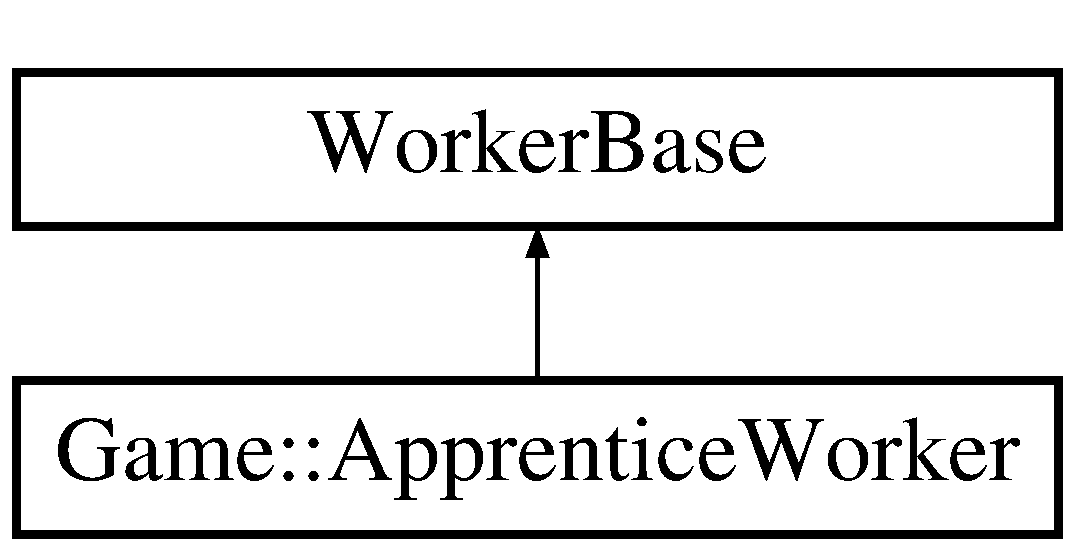
\includegraphics[height=2.000000cm]{class_game_1_1_apprentice_worker}
\end{center}
\end{figure}
\subsection*{Public Member Functions}
\begin{DoxyCompactItemize}
\item 
\hypertarget{class_game_1_1_apprentice_worker_adc6d74ea0acbe8d2237798f256da77ea}{{\bfseries Apprentice\-Worker} (const std\-::shared\-\_\-ptr$<$ \hyperlink{class_game_1_1_game_event_handler}{Game\-Event\-Handler} $>$ \&eventhandler, const std\-::shared\-\_\-ptr$<$ \hyperlink{class_game_1_1_game_object_manager}{Game\-Object\-Manager} $>$ \&objectmanager, const std\-::shared\-\_\-ptr$<$ \hyperlink{class_game_1_1_player}{Player} $>$ \&owner, const int \&tilespaces=1, const Course\-::\-Resource\-Map \&cost=Game\-::\-Const\-Game\-Resource\-Map\-::\-A\-W\-\_\-\-R\-E\-C\-R\-U\-I\-T\-M\-E\-N\-T\-\_\-\-C\-O\-S\-T, const Course\-::\-Resource\-Map\-Double \&efficiency=Game\-::\-Const\-Game\-Resource\-Map\-::\-A\-W\-\_\-\-W\-O\-R\-K\-E\-R\-\_\-\-E\-F\-F\-I\-C\-I\-E\-N\-C\-Y)}\label{class_game_1_1_apprentice_worker_adc6d74ea0acbe8d2237798f256da77ea}

\item 
\hypertarget{class_game_1_1_apprentice_worker_a2389f730db34c05be7dc9bf12e59cc24}{virtual std\-::string {\bfseries get\-Type} () const override}\label{class_game_1_1_apprentice_worker_a2389f730db34c05be7dc9bf12e59cc24}

\item 
\hypertarget{class_game_1_1_apprentice_worker_a0abe6c56acd1e8a876a367e6173e6ca8}{virtual void {\bfseries do\-Special\-Action} () override}\label{class_game_1_1_apprentice_worker_a0abe6c56acd1e8a876a367e6173e6ca8}

\end{DoxyCompactItemize}


\subsection{Detailed Description}
The \hyperlink{class_game_1_1_apprentice_worker}{Apprentice\-Worker} class represents apprentice worker. 

The documentation for this class was generated from the following files\-:\begin{DoxyCompactItemize}
\item 
Workers/apprenticeworker.\-h\item 
Workers/apprenticeworker.\-cpp\end{DoxyCompactItemize}

\hypertarget{class_game_1_1_farm_building}{\section{Game\-:\-:Farm\-Building Class Reference}
\label{class_game_1_1_farm_building}\index{Game\-::\-Farm\-Building@{Game\-::\-Farm\-Building}}
}


The \hyperlink{class_game_1_1_farm_building}{Farm\-Building} class represents a farm.  




{\ttfamily \#include $<$farmbuilding.\-h$>$}

Inheritance diagram for Game\-:\-:Farm\-Building\-:\begin{figure}[H]
\begin{center}
\leavevmode
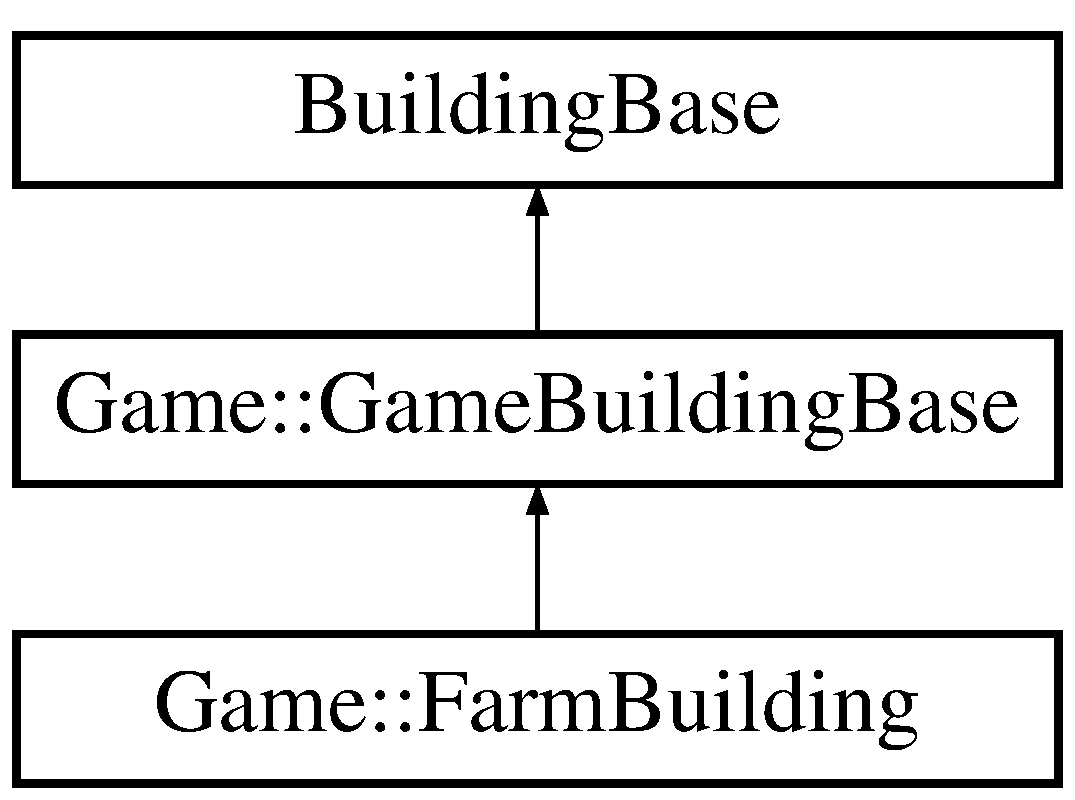
\includegraphics[height=3.000000cm]{class_game_1_1_farm_building}
\end{center}
\end{figure}
\subsection*{Public Member Functions}
\begin{DoxyCompactItemize}
\item 
\hyperlink{class_game_1_1_farm_building_a2930230dbb5607e285ce583fb29addbd}{Farm\-Building} (const std\-::shared\-\_\-ptr$<$ \hyperlink{class_game_1_1_game_event_handler}{Game\-Event\-Handler} $>$ \&eventhandler, const std\-::shared\-\_\-ptr$<$ \hyperlink{class_game_1_1_game_object_manager}{Game\-Object\-Manager} $>$ \&objectmanager, const std\-::shared\-\_\-ptr$<$ \hyperlink{class_game_1_1_player}{Game\-::\-Player} $>$ \&owner, const int \&tilespaces=1, const Course\-::\-Resource\-Map \&buildcost=Game\-::\-Const\-Game\-Resource\-Map\-::\-F\-A\-R\-M\-\_\-\-B\-U\-I\-L\-D\-\_\-\-C\-O\-S\-T, const Course\-::\-Resource\-Map \&production=Game\-::\-Const\-Game\-Resource\-Map\-::\-F\-A\-R\-M\-\_\-\-P\-R\-O\-D\-U\-C\-T\-I\-O\-N)
\begin{DoxyCompactList}\small\item\em \hyperlink{class_game_1_1_farm_building}{Farm\-Building}. \end{DoxyCompactList}\item 
virtual std\-::string \hyperlink{class_game_1_1_farm_building_af251d750c5350eb4295535e81b4b3890}{get\-Type} () const override
\begin{DoxyCompactList}\small\item\em get\-Type \end{DoxyCompactList}\end{DoxyCompactItemize}
\subsection*{Additional Inherited Members}


\subsection{Detailed Description}
The \hyperlink{class_game_1_1_farm_building}{Farm\-Building} class represents a farm. 

\subsection{Constructor \& Destructor Documentation}
\hypertarget{class_game_1_1_farm_building_a2930230dbb5607e285ce583fb29addbd}{\index{Game\-::\-Farm\-Building@{Game\-::\-Farm\-Building}!Farm\-Building@{Farm\-Building}}
\index{Farm\-Building@{Farm\-Building}!Game::FarmBuilding@{Game\-::\-Farm\-Building}}
\subsubsection[{Farm\-Building}]{\setlength{\rightskip}{0pt plus 5cm}Game\-::\-Farm\-Building\-::\-Farm\-Building (
\begin{DoxyParamCaption}
\item[{const std\-::shared\-\_\-ptr$<$ {\bf Game\-Event\-Handler} $>$ \&}]{eventhandler, }
\item[{const std\-::shared\-\_\-ptr$<$ {\bf Game\-Object\-Manager} $>$ \&}]{objectmanager, }
\item[{const std\-::shared\-\_\-ptr$<$ {\bf Game\-::\-Player} $>$ \&}]{owner, }
\item[{const int \&}]{tilespaces = {\ttfamily 1}, }
\item[{const Course\-::\-Resource\-Map \&}]{buildcost = {\ttfamily Game\-:\-:ConstGameResourceMap\-:\-:FARM\-\_\-BUILD\-\_\-COST}, }
\item[{const Course\-::\-Resource\-Map \&}]{production = {\ttfamily Game\-:\-:ConstGameResourceMap\-:\-:FARM\-\_\-PRODUCTION}}
\end{DoxyParamCaption}
)}}\label{class_game_1_1_farm_building_a2930230dbb5607e285ce583fb29addbd}


\hyperlink{class_game_1_1_farm_building}{Farm\-Building}. 


\begin{DoxyParams}{Parameters}
{\em eventhandler} & \\
\hline
{\em objectmanager} & \\
\hline
{\em owner} & \\
\hline
{\em tilespaces} & \\
\hline
{\em buildcost} & \\
\hline
{\em production} & \\
\hline
\end{DoxyParams}


\subsection{Member Function Documentation}
\hypertarget{class_game_1_1_farm_building_af251d750c5350eb4295535e81b4b3890}{\index{Game\-::\-Farm\-Building@{Game\-::\-Farm\-Building}!get\-Type@{get\-Type}}
\index{get\-Type@{get\-Type}!Game::FarmBuilding@{Game\-::\-Farm\-Building}}
\subsubsection[{get\-Type}]{\setlength{\rightskip}{0pt plus 5cm}std\-::string Game\-::\-Farm\-Building\-::get\-Type (
\begin{DoxyParamCaption}
{}
\end{DoxyParamCaption}
) const\hspace{0.3cm}{\ttfamily [override]}, {\ttfamily [virtual]}}}\label{class_game_1_1_farm_building_af251d750c5350eb4295535e81b4b3890}


get\-Type 

\begin{DoxyReturn}{Returns}
type of the building as a string 
\end{DoxyReturn}


The documentation for this class was generated from the following files\-:\begin{DoxyCompactItemize}
\item 
Buildings/farmbuilding.\-h\item 
Buildings/farmbuilding.\-cpp\end{DoxyCompactItemize}

\hypertarget{class_game_1_1_fishing_building}{\section{Game\-:\-:Fishing\-Building Class Reference}
\label{class_game_1_1_fishing_building}\index{Game\-::\-Fishing\-Building@{Game\-::\-Fishing\-Building}}
}


The \hyperlink{class_game_1_1_fishing_building}{Fishing\-Building} class represents a fishing hut.  




{\ttfamily \#include $<$fishingbuilding.\-h$>$}

Inheritance diagram for Game\-:\-:Fishing\-Building\-:\begin{figure}[H]
\begin{center}
\leavevmode
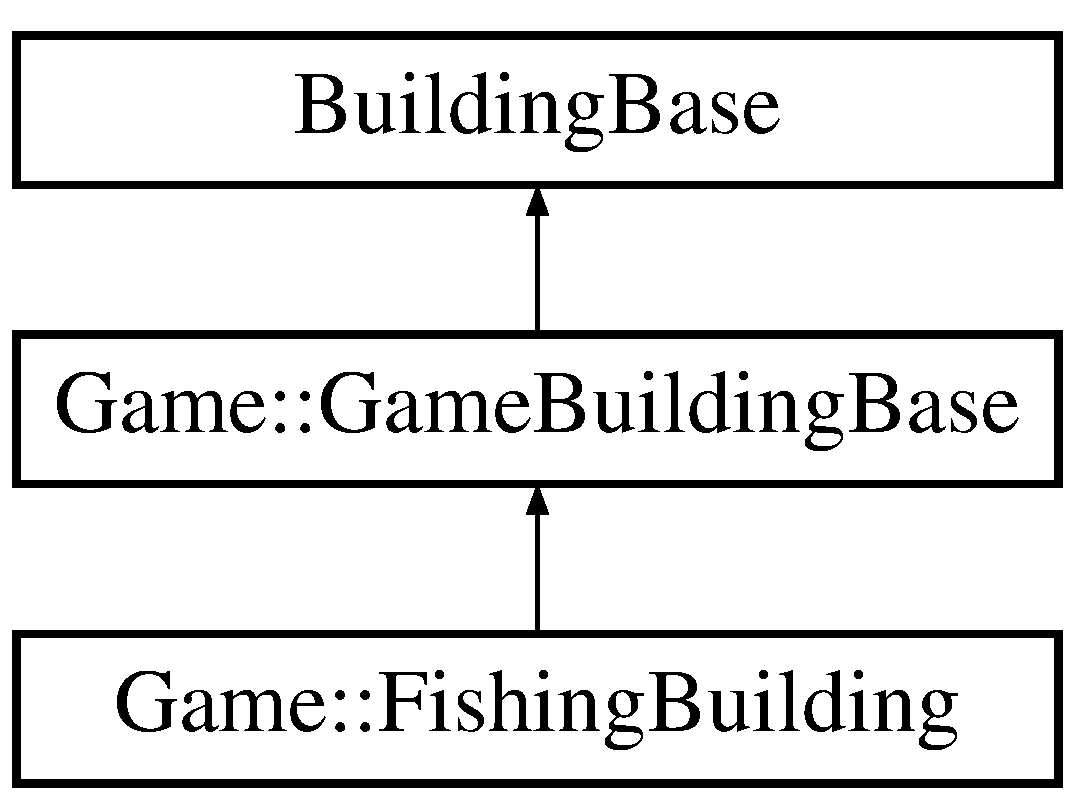
\includegraphics[height=3.000000cm]{class_game_1_1_fishing_building}
\end{center}
\end{figure}
\subsection*{Public Member Functions}
\begin{DoxyCompactItemize}
\item 
\hyperlink{class_game_1_1_fishing_building_a5ab7cea4d687fffabb1cdcec90e5b16f}{Fishing\-Building} (const std\-::shared\-\_\-ptr$<$ \hyperlink{class_game_1_1_game_event_handler}{Game\-Event\-Handler} $>$ \&eventhandler, const std\-::shared\-\_\-ptr$<$ \hyperlink{class_game_1_1_game_object_manager}{Game\-Object\-Manager} $>$ \&objectmanager, const std\-::shared\-\_\-ptr$<$ \hyperlink{class_game_1_1_player}{Game\-::\-Player} $>$ \&owner, const int \&tilespaces=1, const Course\-::\-Resource\-Map \&buildcost=Game\-::\-Const\-Game\-Resource\-Map\-::\-F\-I\-S\-H\-I\-N\-G\-\_\-\-B\-U\-I\-L\-D\-\_\-\-C\-O\-S\-T, const Course\-::\-Resource\-Map \&production=Game\-::\-Const\-Game\-Resource\-Map\-::\-F\-I\-S\-H\-I\-N\-G\-\_\-\-P\-R\-O\-D\-U\-C\-T\-I\-O\-N)
\begin{DoxyCompactList}\small\item\em \hyperlink{class_game_1_1_fishing_building}{Fishing\-Building}. \end{DoxyCompactList}\item 
virtual std\-::string \hyperlink{class_game_1_1_fishing_building_a8e7af836ffde9b004fdf182fc88e2b50}{get\-Type} () const override
\begin{DoxyCompactList}\small\item\em get\-Type \end{DoxyCompactList}\end{DoxyCompactItemize}
\subsection*{Additional Inherited Members}


\subsection{Detailed Description}
The \hyperlink{class_game_1_1_fishing_building}{Fishing\-Building} class represents a fishing hut. 

\subsection{Constructor \& Destructor Documentation}
\hypertarget{class_game_1_1_fishing_building_a5ab7cea4d687fffabb1cdcec90e5b16f}{\index{Game\-::\-Fishing\-Building@{Game\-::\-Fishing\-Building}!Fishing\-Building@{Fishing\-Building}}
\index{Fishing\-Building@{Fishing\-Building}!Game::FishingBuilding@{Game\-::\-Fishing\-Building}}
\subsubsection[{Fishing\-Building}]{\setlength{\rightskip}{0pt plus 5cm}Game\-::\-Fishing\-Building\-::\-Fishing\-Building (
\begin{DoxyParamCaption}
\item[{const std\-::shared\-\_\-ptr$<$ {\bf Game\-Event\-Handler} $>$ \&}]{eventhandler, }
\item[{const std\-::shared\-\_\-ptr$<$ {\bf Game\-Object\-Manager} $>$ \&}]{objectmanager, }
\item[{const std\-::shared\-\_\-ptr$<$ {\bf Game\-::\-Player} $>$ \&}]{owner, }
\item[{const int \&}]{tilespaces = {\ttfamily 1}, }
\item[{const Course\-::\-Resource\-Map \&}]{buildcost = {\ttfamily Game\-:\-:ConstGameResourceMap\-:\-:FISHING\-\_\-BUILD\-\_\-COST}, }
\item[{const Course\-::\-Resource\-Map \&}]{production = {\ttfamily Game\-:\-:ConstGameResourceMap\-:\-:FISHING\-\_\-PRODUCTION}}
\end{DoxyParamCaption}
)}}\label{class_game_1_1_fishing_building_a5ab7cea4d687fffabb1cdcec90e5b16f}


\hyperlink{class_game_1_1_fishing_building}{Fishing\-Building}. 


\begin{DoxyParams}{Parameters}
{\em eventhandler} & \\
\hline
{\em objectmanager} & \\
\hline
{\em owner} & \\
\hline
{\em tilespaces} & \\
\hline
{\em buildcost} & \\
\hline
{\em production} & \\
\hline
\end{DoxyParams}


\subsection{Member Function Documentation}
\hypertarget{class_game_1_1_fishing_building_a8e7af836ffde9b004fdf182fc88e2b50}{\index{Game\-::\-Fishing\-Building@{Game\-::\-Fishing\-Building}!get\-Type@{get\-Type}}
\index{get\-Type@{get\-Type}!Game::FishingBuilding@{Game\-::\-Fishing\-Building}}
\subsubsection[{get\-Type}]{\setlength{\rightskip}{0pt plus 5cm}std\-::string Game\-::\-Fishing\-Building\-::get\-Type (
\begin{DoxyParamCaption}
{}
\end{DoxyParamCaption}
) const\hspace{0.3cm}{\ttfamily [override]}, {\ttfamily [virtual]}}}\label{class_game_1_1_fishing_building_a8e7af836ffde9b004fdf182fc88e2b50}


get\-Type 

\begin{DoxyReturn}{Returns}
type of the building as a string 
\end{DoxyReturn}


The documentation for this class was generated from the following files\-:\begin{DoxyCompactItemize}
\item 
Buildings/fishingbuilding.\-h\item 
Buildings/fishingbuilding.\-cpp\end{DoxyCompactItemize}

\hypertarget{class_game_1_1_foresttile}{\section{Game\-:\-:Foresttile Class Reference}
\label{class_game_1_1_foresttile}\index{Game\-::\-Foresttile@{Game\-::\-Foresttile}}
}


The \hyperlink{class_game_1_1_foresttile}{Foresttile} class represents forest.  




{\ttfamily \#include $<$foresttile.\-h$>$}

Inheritance diagram for Game\-:\-:Foresttile\-:\begin{figure}[H]
\begin{center}
\leavevmode
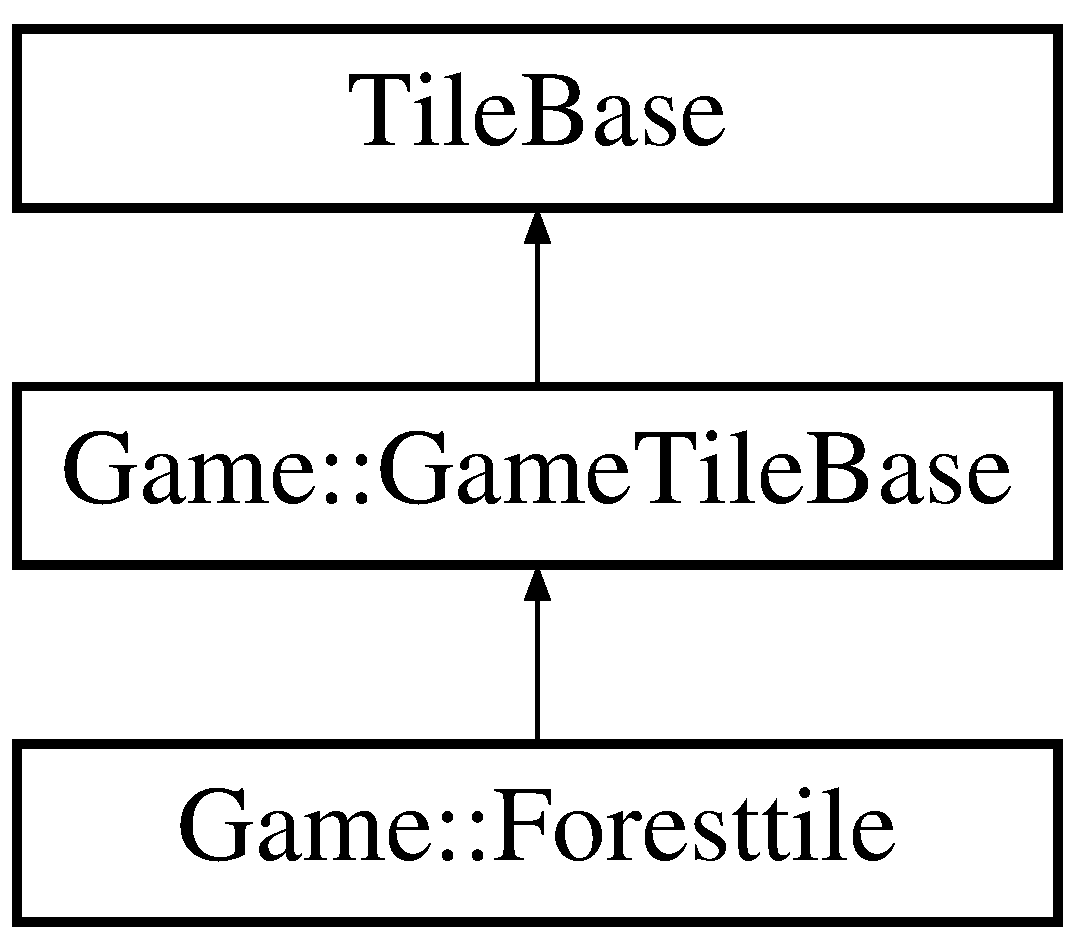
\includegraphics[height=3.000000cm]{class_game_1_1_foresttile}
\end{center}
\end{figure}
\subsection*{Public Member Functions}
\begin{DoxyCompactItemize}
\item 
\hyperlink{class_game_1_1_foresttile_a708533830b5f1255c679dd76baecea0a}{Foresttile} (const Course\-::\-Coordinate \&location, const std\-::shared\-\_\-ptr$<$ \hyperlink{class_game_1_1_game_event_handler}{Game\-Event\-Handler} $>$ \&eventhandler, const std\-::shared\-\_\-ptr$<$ \hyperlink{class_game_1_1_game_object_manager}{Game\-Object\-Manager} $>$ \&objectmanager, const unsigned int \&max\-\_\-build=1, const unsigned int \&max\-\_\-work=4, const Course\-::\-Resource\-Map \&production=Game\-::\-Const\-Game\-Resource\-Map\-::\-T\-I\-L\-E\-\_\-\-B\-P)
\begin{DoxyCompactList}\small\item\em \hyperlink{class_game_1_1_foresttile}{Foresttile}. \end{DoxyCompactList}\item 
virtual std\-::string \hyperlink{class_game_1_1_foresttile_a126210f53c011a036515963ef1216272}{get\-Type} () const override
\begin{DoxyCompactList}\small\item\em get\-Type \end{DoxyCompactList}\end{DoxyCompactItemize}
\subsection*{Additional Inherited Members}


\subsection{Detailed Description}
The \hyperlink{class_game_1_1_foresttile}{Foresttile} class represents forest. 

\subsection{Constructor \& Destructor Documentation}
\hypertarget{class_game_1_1_foresttile_a708533830b5f1255c679dd76baecea0a}{\index{Game\-::\-Foresttile@{Game\-::\-Foresttile}!Foresttile@{Foresttile}}
\index{Foresttile@{Foresttile}!Game::Foresttile@{Game\-::\-Foresttile}}
\subsubsection[{Foresttile}]{\setlength{\rightskip}{0pt plus 5cm}Game\-::\-Foresttile\-::\-Foresttile (
\begin{DoxyParamCaption}
\item[{const Course\-::\-Coordinate \&}]{location, }
\item[{const std\-::shared\-\_\-ptr$<$ {\bf Game\-Event\-Handler} $>$ \&}]{eventhandler, }
\item[{const std\-::shared\-\_\-ptr$<$ {\bf Game\-Object\-Manager} $>$ \&}]{objectmanager, }
\item[{const unsigned int \&}]{max\-\_\-build = {\ttfamily 1}, }
\item[{const unsigned int \&}]{max\-\_\-work = {\ttfamily 4}, }
\item[{const Course\-::\-Resource\-Map \&}]{production = {\ttfamily Game\-:\-:ConstGameResourceMap\-:\-:TILE\-\_\-BP}}
\end{DoxyParamCaption}
)}}\label{class_game_1_1_foresttile_a708533830b5f1255c679dd76baecea0a}


\hyperlink{class_game_1_1_foresttile}{Foresttile}. 


\begin{DoxyParams}{Parameters}
{\em location} & \\
\hline
{\em eventhandler} & \\
\hline
{\em objectmanager} & \\
\hline
{\em max\-\_\-build} & \\
\hline
{\em max\-\_\-work} & \\
\hline
{\em production} & \\
\hline
\end{DoxyParams}


\subsection{Member Function Documentation}
\hypertarget{class_game_1_1_foresttile_a126210f53c011a036515963ef1216272}{\index{Game\-::\-Foresttile@{Game\-::\-Foresttile}!get\-Type@{get\-Type}}
\index{get\-Type@{get\-Type}!Game::Foresttile@{Game\-::\-Foresttile}}
\subsubsection[{get\-Type}]{\setlength{\rightskip}{0pt plus 5cm}std\-::string Game\-::\-Foresttile\-::get\-Type (
\begin{DoxyParamCaption}
{}
\end{DoxyParamCaption}
) const\hspace{0.3cm}{\ttfamily [override]}, {\ttfamily [virtual]}}}\label{class_game_1_1_foresttile_a126210f53c011a036515963ef1216272}


get\-Type 

\begin{DoxyReturn}{Returns}
type of the tile as a string 
\end{DoxyReturn}


The documentation for this class was generated from the following files\-:\begin{DoxyCompactItemize}
\item 
Tiles/foresttile.\-h\item 
Tiles/foresttile.\-cpp\end{DoxyCompactItemize}

\hypertarget{class_game_1_1_game_building_base}{\section{Game\-:\-:Game\-Building\-Base Class Reference}
\label{class_game_1_1_game_building_base}\index{Game\-::\-Game\-Building\-Base@{Game\-::\-Game\-Building\-Base}}
}


The \hyperlink{class_game_1_1_game_building_base}{Game\-Building\-Base} class is a base class for buildings with a sprite/image component. Inherited from Building\-Base.  




{\ttfamily \#include $<$gamebuildingbase.\-h$>$}

Inheritance diagram for Game\-:\-:Game\-Building\-Base\-:\begin{figure}[H]
\begin{center}
\leavevmode
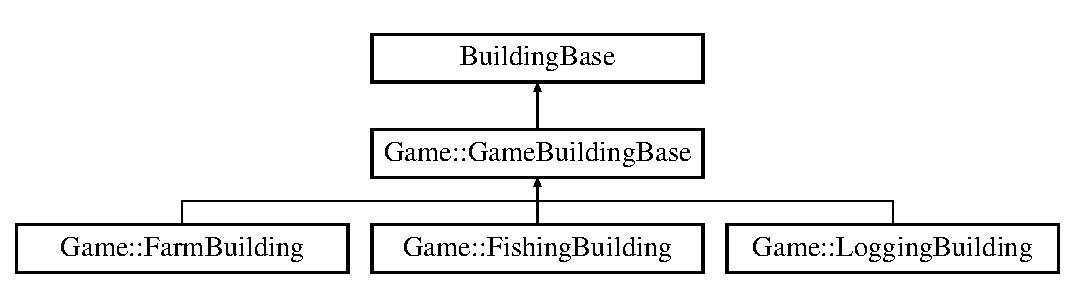
\includegraphics[height=3.000000cm]{class_game_1_1_game_building_base}
\end{center}
\end{figure}
\subsection*{Public Member Functions}
\begin{DoxyCompactItemize}
\item 
\hypertarget{class_game_1_1_game_building_base_a715b5d8f912a668a3e65c5357d524f66}{{\bfseries Game\-Building\-Base} (const std\-::shared\-\_\-ptr$<$ \hyperlink{class_game_1_1_game_event_handler}{Game\-Event\-Handler} $>$ \&eventhandler, const std\-::shared\-\_\-ptr$<$ \hyperlink{class_game_1_1_game_object_manager}{Game\-Object\-Manager} $>$ \&objectmanager, const std\-::shared\-\_\-ptr$<$ \hyperlink{class_game_1_1_player}{Player} $>$ \&owner, const int \&tilespaces=1, const Course\-::\-Resource\-Map \&buildcost=\{\}, const Course\-::\-Resource\-Map \&production=\{\})}\label{class_game_1_1_game_building_base_a715b5d8f912a668a3e65c5357d524f66}

\item 
virtual Q\-Pixmap \hyperlink{class_game_1_1_game_building_base_a8eacd371cae363d396accefb637b04b6}{get\-Sprite} ()
\begin{DoxyCompactList}\small\item\em get\-Sprite Q\-Pix\-Map graphics for buildings \end{DoxyCompactList}\item 
int \hyperlink{class_game_1_1_game_building_base_a5d20b7f0aac3ccbc671c25911a7cd9a1}{get\-Width} ()
\begin{DoxyCompactList}\small\item\em get\-Width \end{DoxyCompactList}\item 
int \hyperlink{class_game_1_1_game_building_base_ac1a873f44dd45d52a919e7638c07498e}{get\-Height} ()
\begin{DoxyCompactList}\small\item\em get\-Height \end{DoxyCompactList}\end{DoxyCompactItemize}
\subsection*{Protected Attributes}
\begin{DoxyCompactItemize}
\item 
\hypertarget{class_game_1_1_game_building_base_a0e218fa83174063e74574ad12a0c9d13}{Q\-Pixmap {\bfseries sprite}}\label{class_game_1_1_game_building_base_a0e218fa83174063e74574ad12a0c9d13}

\item 
\hypertarget{class_game_1_1_game_building_base_a0a56d68ac3f8d437aef06671ce9a19c6}{int {\bfseries width}}\label{class_game_1_1_game_building_base_a0a56d68ac3f8d437aef06671ce9a19c6}

\item 
\hypertarget{class_game_1_1_game_building_base_a1502712620fb26a336d10de32977438e}{int {\bfseries height}}\label{class_game_1_1_game_building_base_a1502712620fb26a336d10de32977438e}

\end{DoxyCompactItemize}


\subsection{Detailed Description}
The \hyperlink{class_game_1_1_game_building_base}{Game\-Building\-Base} class is a base class for buildings with a sprite/image component. Inherited from Building\-Base. 

\subsection{Member Function Documentation}
\hypertarget{class_game_1_1_game_building_base_ac1a873f44dd45d52a919e7638c07498e}{\index{Game\-::\-Game\-Building\-Base@{Game\-::\-Game\-Building\-Base}!get\-Height@{get\-Height}}
\index{get\-Height@{get\-Height}!Game::GameBuildingBase@{Game\-::\-Game\-Building\-Base}}
\subsubsection[{get\-Height}]{\setlength{\rightskip}{0pt plus 5cm}int Game\-::\-Game\-Building\-Base\-::get\-Height (
\begin{DoxyParamCaption}
{}
\end{DoxyParamCaption}
)}}\label{class_game_1_1_game_building_base_ac1a873f44dd45d52a919e7638c07498e}


get\-Height 

\begin{DoxyReturn}{Returns}
the height of the sprite image 
\end{DoxyReturn}
\hypertarget{class_game_1_1_game_building_base_a8eacd371cae363d396accefb637b04b6}{\index{Game\-::\-Game\-Building\-Base@{Game\-::\-Game\-Building\-Base}!get\-Sprite@{get\-Sprite}}
\index{get\-Sprite@{get\-Sprite}!Game::GameBuildingBase@{Game\-::\-Game\-Building\-Base}}
\subsubsection[{get\-Sprite}]{\setlength{\rightskip}{0pt plus 5cm}Q\-Pixmap Game\-::\-Game\-Building\-Base\-::get\-Sprite (
\begin{DoxyParamCaption}
{}
\end{DoxyParamCaption}
)\hspace{0.3cm}{\ttfamily [virtual]}}}\label{class_game_1_1_game_building_base_a8eacd371cae363d396accefb637b04b6}


get\-Sprite Q\-Pix\-Map graphics for buildings 

\begin{DoxyReturn}{Returns}
returns the sprite 
\end{DoxyReturn}
\hypertarget{class_game_1_1_game_building_base_a5d20b7f0aac3ccbc671c25911a7cd9a1}{\index{Game\-::\-Game\-Building\-Base@{Game\-::\-Game\-Building\-Base}!get\-Width@{get\-Width}}
\index{get\-Width@{get\-Width}!Game::GameBuildingBase@{Game\-::\-Game\-Building\-Base}}
\subsubsection[{get\-Width}]{\setlength{\rightskip}{0pt plus 5cm}int Game\-::\-Game\-Building\-Base\-::get\-Width (
\begin{DoxyParamCaption}
{}
\end{DoxyParamCaption}
)}}\label{class_game_1_1_game_building_base_a5d20b7f0aac3ccbc671c25911a7cd9a1}


get\-Width 

\begin{DoxyReturn}{Returns}
the width of the sprite image 
\end{DoxyReturn}


The documentation for this class was generated from the following files\-:\begin{DoxyCompactItemize}
\item 
gamebuildingbase.\-h\item 
gamebuildingbase.\-cpp\end{DoxyCompactItemize}

\hypertarget{class_game_1_1_game_event_handler}{\section{Game\-:\-:Game\-Event\-Handler Class Reference}
\label{class_game_1_1_game_event_handler}\index{Game\-::\-Game\-Event\-Handler@{Game\-::\-Game\-Event\-Handler}}
}


The \hyperlink{class_game_1_1_game_event_handler}{Game\-Event\-Handler} class interface inherited from i\-Game\-Event\-Handler.  




{\ttfamily \#include $<$gameeventhandler.\-h$>$}

Inheritance diagram for Game\-:\-:Game\-Event\-Handler\-:\begin{figure}[H]
\begin{center}
\leavevmode
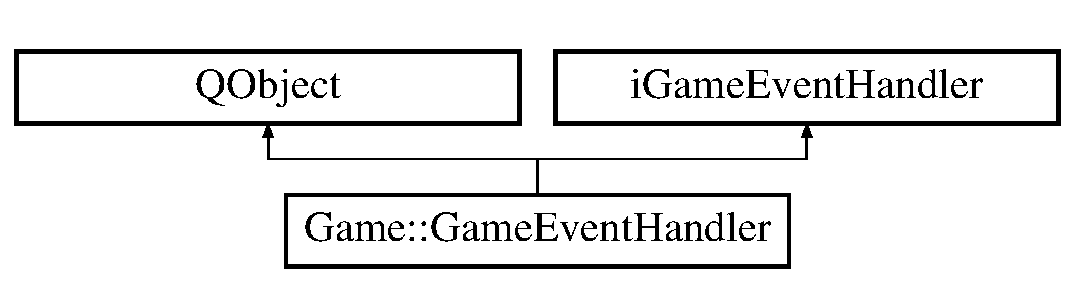
\includegraphics[height=2.000000cm]{class_game_1_1_game_event_handler}
\end{center}
\end{figure}
\subsection*{Signals}
\begin{DoxyCompactItemize}
\item 
\hypertarget{class_game_1_1_game_event_handler_aa66e8120504a75349d8a4281758f2996}{void \hyperlink{class_game_1_1_game_event_handler_aa66e8120504a75349d8a4281758f2996}{game\-Message} (std\-::string)}\label{class_game_1_1_game_event_handler_aa66e8120504a75349d8a4281758f2996}

\begin{DoxyCompactList}\small\item\em game\-Message passes a message (string) to connected components \end{DoxyCompactList}\item 
\hypertarget{class_game_1_1_game_event_handler_a84188b624b591fb2d354e89e85fb81ba}{void \hyperlink{class_game_1_1_game_event_handler_a84188b624b591fb2d354e89e85fb81ba}{game\-Over} (game\-Over\-State)}\label{class_game_1_1_game_event_handler_a84188b624b591fb2d354e89e85fb81ba}

\begin{DoxyCompactList}\small\item\em game\-Over passes information of the state that the game ended with \end{DoxyCompactList}\end{DoxyCompactItemize}
\subsection*{Public Member Functions}
\begin{DoxyCompactItemize}
\item 
\hyperlink{class_game_1_1_game_event_handler_a26aed05051abfec41c863fc8073e324b}{Game\-Event\-Handler} (std\-::shared\-\_\-ptr$<$ \hyperlink{class_game_1_1_game_object_manager}{Game\-Object\-Manager} $>$ manager, Q\-Object $\ast$parent=nullptr)
\begin{DoxyCompactList}\small\item\em \hyperlink{class_game_1_1_game_event_handler}{Game\-Event\-Handler}. \end{DoxyCompactList}\item 
virtual bool \hyperlink{class_game_1_1_game_event_handler_a94426aa16bad3385bc3d75249596325c}{modify\-Resource} (std\-::shared\-\_\-ptr$<$ Course\-::\-Player\-Base $>$ player, Course\-::\-Basic\-Resource resource, int amount)
\begin{DoxyCompactList}\small\item\em modify\-Resource \end{DoxyCompactList}\item 
virtual bool \hyperlink{class_game_1_1_game_event_handler_af2f37590702d555bb6635a6a7793ebb2}{modify\-Resources} (std\-::shared\-\_\-ptr$<$ Course\-::\-Player\-Base $>$ player, Course\-::\-Resource\-Map resources)
\begin{DoxyCompactList}\small\item\em modify\-Resources \end{DoxyCompactList}\item 
\hypertarget{class_game_1_1_game_event_handler_a30de50de65075fe9e5c76ef83ff638a7}{void \hyperlink{class_game_1_1_game_event_handler_a30de50de65075fe9e5c76ef83ff638a7}{end\-Turn} ()}\label{class_game_1_1_game_event_handler_a30de50de65075fe9e5c76ef83ff638a7}

\begin{DoxyCompactList}\small\item\em end\-Turn increases turn count \end{DoxyCompactList}\item 
int \hyperlink{class_game_1_1_game_event_handler_a261195d24462d7d0921cf38cea1b2c2b}{throw\-Dice} ()
\begin{DoxyCompactList}\small\item\em throw\-Dice \end{DoxyCompactList}\item 
int \hyperlink{class_game_1_1_game_event_handler_a991f80f0f775aafebcda3648d23bcd34}{get\-Dice\-Value} ()
\begin{DoxyCompactList}\small\item\em get\-Dice\-Value \end{DoxyCompactList}\item 
int \hyperlink{class_game_1_1_game_event_handler_a6ec04e17ce2ad5e01e7ff295228f2e93}{get\-Turn} ()
\begin{DoxyCompactList}\small\item\em get\-Turn \end{DoxyCompactList}\item 
bool \hyperlink{class_game_1_1_game_event_handler_adc5c0fcca540aecee10f4f686cd75a8a}{get\-Thrown} ()
\begin{DoxyCompactList}\small\item\em get\-Thrown \end{DoxyCompactList}\item 
bool \hyperlink{class_game_1_1_game_event_handler_a92a48620bbbed7ada1723c4fccd1cd12}{get\-Player\-Moved} ()
\begin{DoxyCompactList}\small\item\em get\-Player\-Moved \end{DoxyCompactList}\item 
bool \hyperlink{class_game_1_1_game_event_handler_a9795d3f9e717f6c25f4ce04364f805b7}{is\-Moving} ()
\begin{DoxyCompactList}\small\item\em is\-Moving \end{DoxyCompactList}\item 
bool \hyperlink{class_game_1_1_game_event_handler_af885960b5f0a12cfb8d0a66aaabb830d}{is\-Building} ()
\begin{DoxyCompactList}\small\item\em is\-Building \end{DoxyCompactList}\item 
bool \hyperlink{class_game_1_1_game_event_handler_a30283da07c58c1de52d5a2ed61fd0577}{get\-Player\-Built} ()
\begin{DoxyCompactList}\small\item\em get\-Player\-Built \end{DoxyCompactList}\item 
bool \hyperlink{class_game_1_1_game_event_handler_ae08a601526a33a4416258d258976ed50}{get\-Player\-Searched} ()
\begin{DoxyCompactList}\small\item\em get\-Player\-Searched \end{DoxyCompactList}\item 
bool \hyperlink{class_game_1_1_game_event_handler_a603e124ff876bcad84bc3360124f707b}{is\-Searching} ()
\begin{DoxyCompactList}\small\item\em is\-Searching \end{DoxyCompactList}\item 
bool \hyperlink{class_game_1_1_game_event_handler_a32e3c3c3f8a7dc3d73befa8f899197cb}{is\-Hiring} ()
\begin{DoxyCompactList}\small\item\em is\-Hiring \end{DoxyCompactList}\item 
bool \hyperlink{class_game_1_1_game_event_handler_a158bbaf5035c67ea7b298e9962b8f55f}{get\-Hired} ()
\begin{DoxyCompactList}\small\item\em get\-Hired \end{DoxyCompactList}\item 
std\-::string \hyperlink{class_game_1_1_game_event_handler_ab485ab211069cdb82d912a05ff1cfe50}{get\-Worker\-Type} ()
\begin{DoxyCompactList}\small\item\em get\-Worker\-Type \end{DoxyCompactList}\item 
void \hyperlink{class_game_1_1_game_event_handler_ac3d2b6edba2a72379753ee6cf31d09d3}{set\-Thrown} (bool x)
\begin{DoxyCompactList}\small\item\em set\-Thrown \end{DoxyCompactList}\item 
void \hyperlink{class_game_1_1_game_event_handler_a1ebcaa75d732a1a65403d8abd34e4ce2}{set\-Player\-Moved} (bool x)
\begin{DoxyCompactList}\small\item\em set\-Player\-Moved \end{DoxyCompactList}\item 
void \hyperlink{class_game_1_1_game_event_handler_a99683723d5d65e7d21e5fa1a155d2186}{set\-Player\-Built} (bool x)
\begin{DoxyCompactList}\small\item\em set\-Player\-Built \end{DoxyCompactList}\item 
void \hyperlink{class_game_1_1_game_event_handler_a55e45f31053d73f476b8b4a791a0c0a0}{set\-Moving} (bool x)
\begin{DoxyCompactList}\small\item\em set\-Moving \end{DoxyCompactList}\item 
void \hyperlink{class_game_1_1_game_event_handler_a245850510b1043fd39beaa470b129421}{set\-Building\-State} (bool x)
\begin{DoxyCompactList}\small\item\em set\-Building\-State \end{DoxyCompactList}\item 
void \hyperlink{class_game_1_1_game_event_handler_a41926d8f979f3475d1917d4e6c467cdc}{set\-Selected\-Building\-Type} (std\-::string building\-Type)
\begin{DoxyCompactList}\small\item\em set\-Selected\-Building\-Type \end{DoxyCompactList}\item 
void \hyperlink{class_game_1_1_game_event_handler_a7a92ee4a45984a10990cc67fa25156b1}{set\-Searching} (bool x)
\begin{DoxyCompactList}\small\item\em set\-Searching \end{DoxyCompactList}\item 
void \hyperlink{class_game_1_1_game_event_handler_a70bd7161dcab377c9208d4d0ed098819}{set\-Player\-Searched} (bool x)
\begin{DoxyCompactList}\small\item\em set\-Player\-Searched \end{DoxyCompactList}\item 
void \hyperlink{class_game_1_1_game_event_handler_ac8c930bb1e2c019e2fc8bf83e46cfd9d}{set\-Player\-Hired} (bool x)
\begin{DoxyCompactList}\small\item\em set\-Player\-Hired \end{DoxyCompactList}\item 
void \hyperlink{class_game_1_1_game_event_handler_a71d75a9e789a8fbf1475ac3c932030bb}{set\-Hiring} (bool x)
\begin{DoxyCompactList}\small\item\em set\-Hiring \end{DoxyCompactList}\item 
void \hyperlink{class_game_1_1_game_event_handler_a57dbd2bd7edf4c42cf4a3d69e3eeaffe}{set\-Worker\-Type} (std\-::string type)
\begin{DoxyCompactList}\small\item\em set\-Worker\-Type \end{DoxyCompactList}\end{DoxyCompactItemize}


\subsection{Detailed Description}
The \hyperlink{class_game_1_1_game_event_handler}{Game\-Event\-Handler} class interface inherited from i\-Game\-Event\-Handler. 

\subsection{Constructor \& Destructor Documentation}
\hypertarget{class_game_1_1_game_event_handler_a26aed05051abfec41c863fc8073e324b}{\index{Game\-::\-Game\-Event\-Handler@{Game\-::\-Game\-Event\-Handler}!Game\-Event\-Handler@{Game\-Event\-Handler}}
\index{Game\-Event\-Handler@{Game\-Event\-Handler}!Game::GameEventHandler@{Game\-::\-Game\-Event\-Handler}}
\subsubsection[{Game\-Event\-Handler}]{\setlength{\rightskip}{0pt plus 5cm}Game\-::\-Game\-Event\-Handler\-::\-Game\-Event\-Handler (
\begin{DoxyParamCaption}
\item[{std\-::shared\-\_\-ptr$<$ {\bf Game\-Object\-Manager} $>$}]{manager, }
\item[{Q\-Object $\ast$}]{parent = {\ttfamily nullptr}}
\end{DoxyParamCaption}
)}}\label{class_game_1_1_game_event_handler_a26aed05051abfec41c863fc8073e324b}


\hyperlink{class_game_1_1_game_event_handler}{Game\-Event\-Handler}. 


\begin{DoxyParams}{Parameters}
{\em manager} & points to the game's object manager \\
\hline
{\em parent} & \\
\hline
\end{DoxyParams}


\subsection{Member Function Documentation}
\hypertarget{class_game_1_1_game_event_handler_a991f80f0f775aafebcda3648d23bcd34}{\index{Game\-::\-Game\-Event\-Handler@{Game\-::\-Game\-Event\-Handler}!get\-Dice\-Value@{get\-Dice\-Value}}
\index{get\-Dice\-Value@{get\-Dice\-Value}!Game::GameEventHandler@{Game\-::\-Game\-Event\-Handler}}
\subsubsection[{get\-Dice\-Value}]{\setlength{\rightskip}{0pt plus 5cm}int Game\-::\-Game\-Event\-Handler\-::get\-Dice\-Value (
\begin{DoxyParamCaption}
{}
\end{DoxyParamCaption}
)}}\label{class_game_1_1_game_event_handler_a991f80f0f775aafebcda3648d23bcd34}


get\-Dice\-Value 

\begin{DoxyReturn}{Returns}
the value of the dice 
\end{DoxyReturn}
\hypertarget{class_game_1_1_game_event_handler_a158bbaf5035c67ea7b298e9962b8f55f}{\index{Game\-::\-Game\-Event\-Handler@{Game\-::\-Game\-Event\-Handler}!get\-Hired@{get\-Hired}}
\index{get\-Hired@{get\-Hired}!Game::GameEventHandler@{Game\-::\-Game\-Event\-Handler}}
\subsubsection[{get\-Hired}]{\setlength{\rightskip}{0pt plus 5cm}bool Game\-::\-Game\-Event\-Handler\-::get\-Hired (
\begin{DoxyParamCaption}
{}
\end{DoxyParamCaption}
)}}\label{class_game_1_1_game_event_handler_a158bbaf5035c67ea7b298e9962b8f55f}


get\-Hired 

\begin{DoxyReturn}{Returns}
true, if player has hired, false if not 
\end{DoxyReturn}
\hypertarget{class_game_1_1_game_event_handler_a30283da07c58c1de52d5a2ed61fd0577}{\index{Game\-::\-Game\-Event\-Handler@{Game\-::\-Game\-Event\-Handler}!get\-Player\-Built@{get\-Player\-Built}}
\index{get\-Player\-Built@{get\-Player\-Built}!Game::GameEventHandler@{Game\-::\-Game\-Event\-Handler}}
\subsubsection[{get\-Player\-Built}]{\setlength{\rightskip}{0pt plus 5cm}bool Game\-::\-Game\-Event\-Handler\-::get\-Player\-Built (
\begin{DoxyParamCaption}
{}
\end{DoxyParamCaption}
)}}\label{class_game_1_1_game_event_handler_a30283da07c58c1de52d5a2ed61fd0577}


get\-Player\-Built 

\begin{DoxyReturn}{Returns}
true, if player has built, false if not 
\end{DoxyReturn}
\hypertarget{class_game_1_1_game_event_handler_a92a48620bbbed7ada1723c4fccd1cd12}{\index{Game\-::\-Game\-Event\-Handler@{Game\-::\-Game\-Event\-Handler}!get\-Player\-Moved@{get\-Player\-Moved}}
\index{get\-Player\-Moved@{get\-Player\-Moved}!Game::GameEventHandler@{Game\-::\-Game\-Event\-Handler}}
\subsubsection[{get\-Player\-Moved}]{\setlength{\rightskip}{0pt plus 5cm}bool Game\-::\-Game\-Event\-Handler\-::get\-Player\-Moved (
\begin{DoxyParamCaption}
{}
\end{DoxyParamCaption}
)}}\label{class_game_1_1_game_event_handler_a92a48620bbbed7ada1723c4fccd1cd12}


get\-Player\-Moved 

\begin{DoxyReturn}{Returns}
true, if player has moved, false if not 
\end{DoxyReturn}
\hypertarget{class_game_1_1_game_event_handler_ae08a601526a33a4416258d258976ed50}{\index{Game\-::\-Game\-Event\-Handler@{Game\-::\-Game\-Event\-Handler}!get\-Player\-Searched@{get\-Player\-Searched}}
\index{get\-Player\-Searched@{get\-Player\-Searched}!Game::GameEventHandler@{Game\-::\-Game\-Event\-Handler}}
\subsubsection[{get\-Player\-Searched}]{\setlength{\rightskip}{0pt plus 5cm}bool Game\-::\-Game\-Event\-Handler\-::get\-Player\-Searched (
\begin{DoxyParamCaption}
{}
\end{DoxyParamCaption}
)}}\label{class_game_1_1_game_event_handler_ae08a601526a33a4416258d258976ed50}


get\-Player\-Searched 

\begin{DoxyReturn}{Returns}
true, if player has searched, false if not 
\end{DoxyReturn}
\hypertarget{class_game_1_1_game_event_handler_adc5c0fcca540aecee10f4f686cd75a8a}{\index{Game\-::\-Game\-Event\-Handler@{Game\-::\-Game\-Event\-Handler}!get\-Thrown@{get\-Thrown}}
\index{get\-Thrown@{get\-Thrown}!Game::GameEventHandler@{Game\-::\-Game\-Event\-Handler}}
\subsubsection[{get\-Thrown}]{\setlength{\rightskip}{0pt plus 5cm}bool Game\-::\-Game\-Event\-Handler\-::get\-Thrown (
\begin{DoxyParamCaption}
{}
\end{DoxyParamCaption}
)}}\label{class_game_1_1_game_event_handler_adc5c0fcca540aecee10f4f686cd75a8a}


get\-Thrown 

\begin{DoxyReturn}{Returns}
true, if player has thrown, false if not 
\end{DoxyReturn}
\hypertarget{class_game_1_1_game_event_handler_a6ec04e17ce2ad5e01e7ff295228f2e93}{\index{Game\-::\-Game\-Event\-Handler@{Game\-::\-Game\-Event\-Handler}!get\-Turn@{get\-Turn}}
\index{get\-Turn@{get\-Turn}!Game::GameEventHandler@{Game\-::\-Game\-Event\-Handler}}
\subsubsection[{get\-Turn}]{\setlength{\rightskip}{0pt plus 5cm}int Game\-::\-Game\-Event\-Handler\-::get\-Turn (
\begin{DoxyParamCaption}
{}
\end{DoxyParamCaption}
)}}\label{class_game_1_1_game_event_handler_a6ec04e17ce2ad5e01e7ff295228f2e93}


get\-Turn 

\begin{DoxyReturn}{Returns}
current turn 
\end{DoxyReturn}
\hypertarget{class_game_1_1_game_event_handler_ab485ab211069cdb82d912a05ff1cfe50}{\index{Game\-::\-Game\-Event\-Handler@{Game\-::\-Game\-Event\-Handler}!get\-Worker\-Type@{get\-Worker\-Type}}
\index{get\-Worker\-Type@{get\-Worker\-Type}!Game::GameEventHandler@{Game\-::\-Game\-Event\-Handler}}
\subsubsection[{get\-Worker\-Type}]{\setlength{\rightskip}{0pt plus 5cm}std\-::string Game\-::\-Game\-Event\-Handler\-::get\-Worker\-Type (
\begin{DoxyParamCaption}
{}
\end{DoxyParamCaption}
)}}\label{class_game_1_1_game_event_handler_ab485ab211069cdb82d912a05ff1cfe50}


get\-Worker\-Type 

\begin{DoxyReturn}{Returns}
the Type of worker that has been selected 
\end{DoxyReturn}
\hypertarget{class_game_1_1_game_event_handler_af885960b5f0a12cfb8d0a66aaabb830d}{\index{Game\-::\-Game\-Event\-Handler@{Game\-::\-Game\-Event\-Handler}!is\-Building@{is\-Building}}
\index{is\-Building@{is\-Building}!Game::GameEventHandler@{Game\-::\-Game\-Event\-Handler}}
\subsubsection[{is\-Building}]{\setlength{\rightskip}{0pt plus 5cm}bool Game\-::\-Game\-Event\-Handler\-::is\-Building (
\begin{DoxyParamCaption}
{}
\end{DoxyParamCaption}
)}}\label{class_game_1_1_game_event_handler_af885960b5f0a12cfb8d0a66aaabb830d}


is\-Building 

\begin{DoxyReturn}{Returns}
true, if player is building, false if not 
\end{DoxyReturn}
\hypertarget{class_game_1_1_game_event_handler_a32e3c3c3f8a7dc3d73befa8f899197cb}{\index{Game\-::\-Game\-Event\-Handler@{Game\-::\-Game\-Event\-Handler}!is\-Hiring@{is\-Hiring}}
\index{is\-Hiring@{is\-Hiring}!Game::GameEventHandler@{Game\-::\-Game\-Event\-Handler}}
\subsubsection[{is\-Hiring}]{\setlength{\rightskip}{0pt plus 5cm}bool Game\-::\-Game\-Event\-Handler\-::is\-Hiring (
\begin{DoxyParamCaption}
{}
\end{DoxyParamCaption}
)}}\label{class_game_1_1_game_event_handler_a32e3c3c3f8a7dc3d73befa8f899197cb}


is\-Hiring 

\begin{DoxyReturn}{Returns}
true, if player is hiring, false if not 
\end{DoxyReturn}
\hypertarget{class_game_1_1_game_event_handler_a9795d3f9e717f6c25f4ce04364f805b7}{\index{Game\-::\-Game\-Event\-Handler@{Game\-::\-Game\-Event\-Handler}!is\-Moving@{is\-Moving}}
\index{is\-Moving@{is\-Moving}!Game::GameEventHandler@{Game\-::\-Game\-Event\-Handler}}
\subsubsection[{is\-Moving}]{\setlength{\rightskip}{0pt plus 5cm}bool Game\-::\-Game\-Event\-Handler\-::is\-Moving (
\begin{DoxyParamCaption}
{}
\end{DoxyParamCaption}
)}}\label{class_game_1_1_game_event_handler_a9795d3f9e717f6c25f4ce04364f805b7}


is\-Moving 

\begin{DoxyReturn}{Returns}
true, if player is moving, false if not 
\end{DoxyReturn}
\hypertarget{class_game_1_1_game_event_handler_a603e124ff876bcad84bc3360124f707b}{\index{Game\-::\-Game\-Event\-Handler@{Game\-::\-Game\-Event\-Handler}!is\-Searching@{is\-Searching}}
\index{is\-Searching@{is\-Searching}!Game::GameEventHandler@{Game\-::\-Game\-Event\-Handler}}
\subsubsection[{is\-Searching}]{\setlength{\rightskip}{0pt plus 5cm}bool Game\-::\-Game\-Event\-Handler\-::is\-Searching (
\begin{DoxyParamCaption}
{}
\end{DoxyParamCaption}
)}}\label{class_game_1_1_game_event_handler_a603e124ff876bcad84bc3360124f707b}


is\-Searching 

\begin{DoxyReturn}{Returns}
true, if player is searching, false if not 
\end{DoxyReturn}
\hypertarget{class_game_1_1_game_event_handler_a94426aa16bad3385bc3d75249596325c}{\index{Game\-::\-Game\-Event\-Handler@{Game\-::\-Game\-Event\-Handler}!modify\-Resource@{modify\-Resource}}
\index{modify\-Resource@{modify\-Resource}!Game::GameEventHandler@{Game\-::\-Game\-Event\-Handler}}
\subsubsection[{modify\-Resource}]{\setlength{\rightskip}{0pt plus 5cm}bool Game\-::\-Game\-Event\-Handler\-::modify\-Resource (
\begin{DoxyParamCaption}
\item[{std\-::shared\-\_\-ptr$<$ Course\-::\-Player\-Base $>$}]{player, }
\item[{Course\-::\-Basic\-Resource}]{resource, }
\item[{int}]{amount}
\end{DoxyParamCaption}
)\hspace{0.3cm}{\ttfamily [virtual]}}}\label{class_game_1_1_game_event_handler_a94426aa16bad3385bc3d75249596325c}


modify\-Resource 


\begin{DoxyParams}{Parameters}
{\em player} & \\
\hline
{\em resource} & \\
\hline
{\em amount} & \\
\hline
\end{DoxyParams}
\begin{DoxyReturn}{Returns}
true, if modification was successful, false if not used to modify player's one resource by given amount 
\end{DoxyReturn}
\hypertarget{class_game_1_1_game_event_handler_af2f37590702d555bb6635a6a7793ebb2}{\index{Game\-::\-Game\-Event\-Handler@{Game\-::\-Game\-Event\-Handler}!modify\-Resources@{modify\-Resources}}
\index{modify\-Resources@{modify\-Resources}!Game::GameEventHandler@{Game\-::\-Game\-Event\-Handler}}
\subsubsection[{modify\-Resources}]{\setlength{\rightskip}{0pt plus 5cm}bool Game\-::\-Game\-Event\-Handler\-::modify\-Resources (
\begin{DoxyParamCaption}
\item[{std\-::shared\-\_\-ptr$<$ Course\-::\-Player\-Base $>$}]{player, }
\item[{Course\-::\-Resource\-Map}]{resources}
\end{DoxyParamCaption}
)\hspace{0.3cm}{\ttfamily [virtual]}}}\label{class_game_1_1_game_event_handler_af2f37590702d555bb6635a6a7793ebb2}


modify\-Resources 


\begin{DoxyParams}{Parameters}
{\em player} & \\
\hline
{\em resources} & \\
\hline
\end{DoxyParams}
\begin{DoxyReturn}{Returns}
true, if modification was successful, false if not used to add or substract player's resources 
\end{DoxyReturn}
\hypertarget{class_game_1_1_game_event_handler_a245850510b1043fd39beaa470b129421}{\index{Game\-::\-Game\-Event\-Handler@{Game\-::\-Game\-Event\-Handler}!set\-Building\-State@{set\-Building\-State}}
\index{set\-Building\-State@{set\-Building\-State}!Game::GameEventHandler@{Game\-::\-Game\-Event\-Handler}}
\subsubsection[{set\-Building\-State}]{\setlength{\rightskip}{0pt plus 5cm}void Game\-::\-Game\-Event\-Handler\-::set\-Building\-State (
\begin{DoxyParamCaption}
\item[{bool}]{x}
\end{DoxyParamCaption}
)}}\label{class_game_1_1_game_event_handler_a245850510b1043fd39beaa470b129421}


set\-Building\-State 


\begin{DoxyParams}{Parameters}
{\em x} & \\
\hline
\end{DoxyParams}
\hypertarget{class_game_1_1_game_event_handler_a71d75a9e789a8fbf1475ac3c932030bb}{\index{Game\-::\-Game\-Event\-Handler@{Game\-::\-Game\-Event\-Handler}!set\-Hiring@{set\-Hiring}}
\index{set\-Hiring@{set\-Hiring}!Game::GameEventHandler@{Game\-::\-Game\-Event\-Handler}}
\subsubsection[{set\-Hiring}]{\setlength{\rightskip}{0pt plus 5cm}void Game\-::\-Game\-Event\-Handler\-::set\-Hiring (
\begin{DoxyParamCaption}
\item[{bool}]{x}
\end{DoxyParamCaption}
)}}\label{class_game_1_1_game_event_handler_a71d75a9e789a8fbf1475ac3c932030bb}


set\-Hiring 


\begin{DoxyParams}{Parameters}
{\em x} & \\
\hline
\end{DoxyParams}
\hypertarget{class_game_1_1_game_event_handler_a55e45f31053d73f476b8b4a791a0c0a0}{\index{Game\-::\-Game\-Event\-Handler@{Game\-::\-Game\-Event\-Handler}!set\-Moving@{set\-Moving}}
\index{set\-Moving@{set\-Moving}!Game::GameEventHandler@{Game\-::\-Game\-Event\-Handler}}
\subsubsection[{set\-Moving}]{\setlength{\rightskip}{0pt plus 5cm}void Game\-::\-Game\-Event\-Handler\-::set\-Moving (
\begin{DoxyParamCaption}
\item[{bool}]{x}
\end{DoxyParamCaption}
)}}\label{class_game_1_1_game_event_handler_a55e45f31053d73f476b8b4a791a0c0a0}


set\-Moving 


\begin{DoxyParams}{Parameters}
{\em x} & \\
\hline
\end{DoxyParams}
\hypertarget{class_game_1_1_game_event_handler_a99683723d5d65e7d21e5fa1a155d2186}{\index{Game\-::\-Game\-Event\-Handler@{Game\-::\-Game\-Event\-Handler}!set\-Player\-Built@{set\-Player\-Built}}
\index{set\-Player\-Built@{set\-Player\-Built}!Game::GameEventHandler@{Game\-::\-Game\-Event\-Handler}}
\subsubsection[{set\-Player\-Built}]{\setlength{\rightskip}{0pt plus 5cm}void Game\-::\-Game\-Event\-Handler\-::set\-Player\-Built (
\begin{DoxyParamCaption}
\item[{bool}]{x}
\end{DoxyParamCaption}
)}}\label{class_game_1_1_game_event_handler_a99683723d5d65e7d21e5fa1a155d2186}


set\-Player\-Built 


\begin{DoxyParams}{Parameters}
{\em x} & \\
\hline
\end{DoxyParams}
\hypertarget{class_game_1_1_game_event_handler_ac8c930bb1e2c019e2fc8bf83e46cfd9d}{\index{Game\-::\-Game\-Event\-Handler@{Game\-::\-Game\-Event\-Handler}!set\-Player\-Hired@{set\-Player\-Hired}}
\index{set\-Player\-Hired@{set\-Player\-Hired}!Game::GameEventHandler@{Game\-::\-Game\-Event\-Handler}}
\subsubsection[{set\-Player\-Hired}]{\setlength{\rightskip}{0pt plus 5cm}void Game\-::\-Game\-Event\-Handler\-::set\-Player\-Hired (
\begin{DoxyParamCaption}
\item[{bool}]{x}
\end{DoxyParamCaption}
)}}\label{class_game_1_1_game_event_handler_ac8c930bb1e2c019e2fc8bf83e46cfd9d}


set\-Player\-Hired 


\begin{DoxyParams}{Parameters}
{\em x} & \\
\hline
\end{DoxyParams}
\hypertarget{class_game_1_1_game_event_handler_a1ebcaa75d732a1a65403d8abd34e4ce2}{\index{Game\-::\-Game\-Event\-Handler@{Game\-::\-Game\-Event\-Handler}!set\-Player\-Moved@{set\-Player\-Moved}}
\index{set\-Player\-Moved@{set\-Player\-Moved}!Game::GameEventHandler@{Game\-::\-Game\-Event\-Handler}}
\subsubsection[{set\-Player\-Moved}]{\setlength{\rightskip}{0pt plus 5cm}void Game\-::\-Game\-Event\-Handler\-::set\-Player\-Moved (
\begin{DoxyParamCaption}
\item[{bool}]{x}
\end{DoxyParamCaption}
)}}\label{class_game_1_1_game_event_handler_a1ebcaa75d732a1a65403d8abd34e4ce2}


set\-Player\-Moved 


\begin{DoxyParams}{Parameters}
{\em x} & \\
\hline
\end{DoxyParams}
\hypertarget{class_game_1_1_game_event_handler_a70bd7161dcab377c9208d4d0ed098819}{\index{Game\-::\-Game\-Event\-Handler@{Game\-::\-Game\-Event\-Handler}!set\-Player\-Searched@{set\-Player\-Searched}}
\index{set\-Player\-Searched@{set\-Player\-Searched}!Game::GameEventHandler@{Game\-::\-Game\-Event\-Handler}}
\subsubsection[{set\-Player\-Searched}]{\setlength{\rightskip}{0pt plus 5cm}void Game\-::\-Game\-Event\-Handler\-::set\-Player\-Searched (
\begin{DoxyParamCaption}
\item[{bool}]{x}
\end{DoxyParamCaption}
)}}\label{class_game_1_1_game_event_handler_a70bd7161dcab377c9208d4d0ed098819}


set\-Player\-Searched 


\begin{DoxyParams}{Parameters}
{\em x} & \\
\hline
\end{DoxyParams}
\hypertarget{class_game_1_1_game_event_handler_a7a92ee4a45984a10990cc67fa25156b1}{\index{Game\-::\-Game\-Event\-Handler@{Game\-::\-Game\-Event\-Handler}!set\-Searching@{set\-Searching}}
\index{set\-Searching@{set\-Searching}!Game::GameEventHandler@{Game\-::\-Game\-Event\-Handler}}
\subsubsection[{set\-Searching}]{\setlength{\rightskip}{0pt plus 5cm}void Game\-::\-Game\-Event\-Handler\-::set\-Searching (
\begin{DoxyParamCaption}
\item[{bool}]{x}
\end{DoxyParamCaption}
)}}\label{class_game_1_1_game_event_handler_a7a92ee4a45984a10990cc67fa25156b1}


set\-Searching 


\begin{DoxyParams}{Parameters}
{\em x} & \\
\hline
\end{DoxyParams}
\hypertarget{class_game_1_1_game_event_handler_a41926d8f979f3475d1917d4e6c467cdc}{\index{Game\-::\-Game\-Event\-Handler@{Game\-::\-Game\-Event\-Handler}!set\-Selected\-Building\-Type@{set\-Selected\-Building\-Type}}
\index{set\-Selected\-Building\-Type@{set\-Selected\-Building\-Type}!Game::GameEventHandler@{Game\-::\-Game\-Event\-Handler}}
\subsubsection[{set\-Selected\-Building\-Type}]{\setlength{\rightskip}{0pt plus 5cm}void Game\-::\-Game\-Event\-Handler\-::set\-Selected\-Building\-Type (
\begin{DoxyParamCaption}
\item[{std\-::string}]{building\-Type}
\end{DoxyParamCaption}
)}}\label{class_game_1_1_game_event_handler_a41926d8f979f3475d1917d4e6c467cdc}


set\-Selected\-Building\-Type 


\begin{DoxyParams}{Parameters}
{\em building\-Type} & \\
\hline
\end{DoxyParams}
\hypertarget{class_game_1_1_game_event_handler_ac3d2b6edba2a72379753ee6cf31d09d3}{\index{Game\-::\-Game\-Event\-Handler@{Game\-::\-Game\-Event\-Handler}!set\-Thrown@{set\-Thrown}}
\index{set\-Thrown@{set\-Thrown}!Game::GameEventHandler@{Game\-::\-Game\-Event\-Handler}}
\subsubsection[{set\-Thrown}]{\setlength{\rightskip}{0pt plus 5cm}void Game\-::\-Game\-Event\-Handler\-::set\-Thrown (
\begin{DoxyParamCaption}
\item[{bool}]{x}
\end{DoxyParamCaption}
)}}\label{class_game_1_1_game_event_handler_ac3d2b6edba2a72379753ee6cf31d09d3}


set\-Thrown 


\begin{DoxyParams}{Parameters}
{\em x} & \\
\hline
\end{DoxyParams}
\hypertarget{class_game_1_1_game_event_handler_a57dbd2bd7edf4c42cf4a3d69e3eeaffe}{\index{Game\-::\-Game\-Event\-Handler@{Game\-::\-Game\-Event\-Handler}!set\-Worker\-Type@{set\-Worker\-Type}}
\index{set\-Worker\-Type@{set\-Worker\-Type}!Game::GameEventHandler@{Game\-::\-Game\-Event\-Handler}}
\subsubsection[{set\-Worker\-Type}]{\setlength{\rightskip}{0pt plus 5cm}void Game\-::\-Game\-Event\-Handler\-::set\-Worker\-Type (
\begin{DoxyParamCaption}
\item[{std\-::string}]{type}
\end{DoxyParamCaption}
)}}\label{class_game_1_1_game_event_handler_a57dbd2bd7edf4c42cf4a3d69e3eeaffe}


set\-Worker\-Type 


\begin{DoxyParams}{Parameters}
{\em type} & \\
\hline
\end{DoxyParams}
\hypertarget{class_game_1_1_game_event_handler_a261195d24462d7d0921cf38cea1b2c2b}{\index{Game\-::\-Game\-Event\-Handler@{Game\-::\-Game\-Event\-Handler}!throw\-Dice@{throw\-Dice}}
\index{throw\-Dice@{throw\-Dice}!Game::GameEventHandler@{Game\-::\-Game\-Event\-Handler}}
\subsubsection[{throw\-Dice}]{\setlength{\rightskip}{0pt plus 5cm}int Game\-::\-Game\-Event\-Handler\-::throw\-Dice (
\begin{DoxyParamCaption}
{}
\end{DoxyParamCaption}
)}}\label{class_game_1_1_game_event_handler_a261195d24462d7d0921cf38cea1b2c2b}


throw\-Dice 

\begin{DoxyReturn}{Returns}
dice number 
\end{DoxyReturn}


The documentation for this class was generated from the following files\-:\begin{DoxyCompactItemize}
\item 
gameeventhandler.\-h\item 
gameeventhandler.\-cpp\end{DoxyCompactItemize}

\hypertarget{class_game_1_1_game_map_generator}{\section{Game\-:\-:Game\-Map\-Generator Class Reference}
\label{class_game_1_1_game_map_generator}\index{Game\-::\-Game\-Map\-Generator@{Game\-::\-Game\-Map\-Generator}}
}


The \hyperlink{class_game_1_1_game_map_generator}{Game\-Map\-Generator} class creates new game objects that make up the game world.  




{\ttfamily \#include $<$gamemapgenerator.\-h$>$}

Inheritance diagram for Game\-:\-:Game\-Map\-Generator\-:\begin{figure}[H]
\begin{center}
\leavevmode
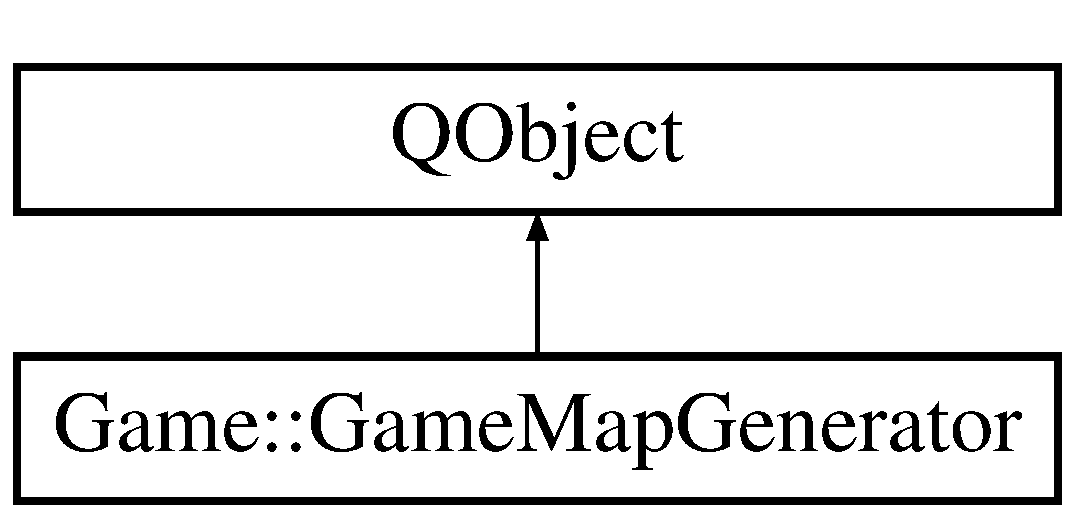
\includegraphics[height=2.000000cm]{class_game_1_1_game_map_generator}
\end{center}
\end{figure}
\subsection*{Signals}
\begin{DoxyCompactItemize}
\item 
\hypertarget{class_game_1_1_game_map_generator_a6e6c320ad1d5678db94d4d2092d92dce}{void \hyperlink{class_game_1_1_game_map_generator_a6e6c320ad1d5678db94d4d2092d92dce}{game\-Message} (std\-::string)}\label{class_game_1_1_game_map_generator_a6e6c320ad1d5678db94d4d2092d92dce}

\begin{DoxyCompactList}\small\item\em game\-Message sends a message (string) to connected slots \end{DoxyCompactList}\end{DoxyCompactItemize}
\subsection*{Public Member Functions}
\begin{DoxyCompactItemize}
\item 
\hyperlink{class_game_1_1_game_map_generator_aa8954c522853a78bc313de335c09a584}{Game\-Map\-Generator} (std\-::shared\-\_\-ptr$<$ \hyperlink{class_game_1_1_game_object_manager}{Game\-Object\-Manager} $>$ obj\-Manager, std\-::shared\-\_\-ptr$<$ \hyperlink{class_game_1_1_game_event_handler}{Game\-Event\-Handler} $>$ event\-Handler, Q\-Object $\ast$parent=nullptr)
\begin{DoxyCompactList}\small\item\em \hyperlink{class_game_1_1_game_map_generator}{Game\-Map\-Generator}. \end{DoxyCompactList}\item 
\hypertarget{class_game_1_1_game_map_generator_a074eff0c7eccb9f9d0fc356d0f08ed3b}{void \hyperlink{class_game_1_1_game_map_generator_a074eff0c7eccb9f9d0fc356d0f08ed3b}{create\-Map\-Objects} ()}\label{class_game_1_1_game_map_generator_a074eff0c7eccb9f9d0fc356d0f08ed3b}

\begin{DoxyCompactList}\small\item\em create\-Map\-Objects Creates tiles according to their corresponding integer values in map\-Template matrix. \end{DoxyCompactList}\item 
void \hyperlink{class_game_1_1_game_map_generator_afad5aeb1e5bcfba092f215875738151d}{create\-Building} (Course\-::\-Coordinate location)
\begin{DoxyCompactList}\small\item\em create\-Building \end{DoxyCompactList}\item 
Course\-::\-Coordinate \hyperlink{class_game_1_1_game_map_generator_ac8afc913679cc83e1e9fdb0fe2ddacbd}{get\-Random\-Map\-Coordinate} ()
\begin{DoxyCompactList}\small\item\em get\-Random\-Map\-Coordinate \end{DoxyCompactList}\item 
\hypertarget{class_game_1_1_game_map_generator_ab39d179c38d46d2289822aff823f0ad9}{void {\bfseries set\-Treasure} (int amount)}\label{class_game_1_1_game_map_generator_ab39d179c38d46d2289822aff823f0ad9}

\item 
\hypertarget{class_game_1_1_game_map_generator_aa3794987e119dd0a7042c96d71df5e7f}{void {\bfseries set\-Robber} (int amount)}\label{class_game_1_1_game_map_generator_aa3794987e119dd0a7042c96d71df5e7f}

\item 
void \hyperlink{class_game_1_1_game_map_generator_a1b301db62c61705ea32830a1db98a716}{create\-Player} (Course\-::\-Coordinate location)
\begin{DoxyCompactList}\small\item\em create\-Player \end{DoxyCompactList}\item 
void \hyperlink{class_game_1_1_game_map_generator_aa5c293a4b89a06f0ae21525e01beffad}{create\-Worker} (std\-::shared\-\_\-ptr$<$ \hyperlink{class_game_1_1_game_tile_base}{Game\-Tile\-Base} $>$ target\-Tile)
\begin{DoxyCompactList}\small\item\em create\-Worker \end{DoxyCompactList}\end{DoxyCompactItemize}


\subsection{Detailed Description}
The \hyperlink{class_game_1_1_game_map_generator}{Game\-Map\-Generator} class creates new game objects that make up the game world. 

\subsection{Constructor \& Destructor Documentation}
\hypertarget{class_game_1_1_game_map_generator_aa8954c522853a78bc313de335c09a584}{\index{Game\-::\-Game\-Map\-Generator@{Game\-::\-Game\-Map\-Generator}!Game\-Map\-Generator@{Game\-Map\-Generator}}
\index{Game\-Map\-Generator@{Game\-Map\-Generator}!Game::GameMapGenerator@{Game\-::\-Game\-Map\-Generator}}
\subsubsection[{Game\-Map\-Generator}]{\setlength{\rightskip}{0pt plus 5cm}Game\-::\-Game\-Map\-Generator\-::\-Game\-Map\-Generator (
\begin{DoxyParamCaption}
\item[{std\-::shared\-\_\-ptr$<$ {\bf Game\-Object\-Manager} $>$}]{obj\-Manager, }
\item[{std\-::shared\-\_\-ptr$<$ {\bf Game\-Event\-Handler} $>$}]{event\-Handler, }
\item[{Q\-Object $\ast$}]{parent = {\ttfamily nullptr}}
\end{DoxyParamCaption}
)}}\label{class_game_1_1_game_map_generator_aa8954c522853a78bc313de335c09a584}


\hyperlink{class_game_1_1_game_map_generator}{Game\-Map\-Generator}. 


\begin{DoxyParams}{Parameters}
{\em obj\-Manager} & \\
\hline
{\em event\-Handler} & \\
\hline
{\em parent} & \\
\hline
\end{DoxyParams}


\subsection{Member Function Documentation}
\hypertarget{class_game_1_1_game_map_generator_afad5aeb1e5bcfba092f215875738151d}{\index{Game\-::\-Game\-Map\-Generator@{Game\-::\-Game\-Map\-Generator}!create\-Building@{create\-Building}}
\index{create\-Building@{create\-Building}!Game::GameMapGenerator@{Game\-::\-Game\-Map\-Generator}}
\subsubsection[{create\-Building}]{\setlength{\rightskip}{0pt plus 5cm}void Game\-::\-Game\-Map\-Generator\-::create\-Building (
\begin{DoxyParamCaption}
\item[{Course\-::\-Coordinate}]{location}
\end{DoxyParamCaption}
)}}\label{class_game_1_1_game_map_generator_afad5aeb1e5bcfba092f215875738151d}


create\-Building 


\begin{DoxyParams}{Parameters}
{\em location} & Creates a building to the tile in the given location. \\
\hline
\end{DoxyParams}
\hypertarget{class_game_1_1_game_map_generator_a1b301db62c61705ea32830a1db98a716}{\index{Game\-::\-Game\-Map\-Generator@{Game\-::\-Game\-Map\-Generator}!create\-Player@{create\-Player}}
\index{create\-Player@{create\-Player}!Game::GameMapGenerator@{Game\-::\-Game\-Map\-Generator}}
\subsubsection[{create\-Player}]{\setlength{\rightskip}{0pt plus 5cm}void Game\-::\-Game\-Map\-Generator\-::create\-Player (
\begin{DoxyParamCaption}
\item[{Course\-::\-Coordinate}]{location}
\end{DoxyParamCaption}
)}}\label{class_game_1_1_game_map_generator_a1b301db62c61705ea32830a1db98a716}


create\-Player 


\begin{DoxyParams}{Parameters}
{\em location} & Creates a new \hyperlink{class_game_1_1_player}{Player} character and adds it to object manager \\
\hline
\end{DoxyParams}
\hypertarget{class_game_1_1_game_map_generator_aa5c293a4b89a06f0ae21525e01beffad}{\index{Game\-::\-Game\-Map\-Generator@{Game\-::\-Game\-Map\-Generator}!create\-Worker@{create\-Worker}}
\index{create\-Worker@{create\-Worker}!Game::GameMapGenerator@{Game\-::\-Game\-Map\-Generator}}
\subsubsection[{create\-Worker}]{\setlength{\rightskip}{0pt plus 5cm}void Game\-::\-Game\-Map\-Generator\-::create\-Worker (
\begin{DoxyParamCaption}
\item[{std\-::shared\-\_\-ptr$<$ {\bf Game\-Tile\-Base} $>$}]{target\-Tile}
\end{DoxyParamCaption}
)}}\label{class_game_1_1_game_map_generator_aa5c293a4b89a06f0ae21525e01beffad}


create\-Worker 


\begin{DoxyParams}{Parameters}
{\em target\-Tile} & Creates a new worker according to the selected worker type in event\-Handler and adds it to the given Tile's list of workers. \\
\hline
\end{DoxyParams}
\hypertarget{class_game_1_1_game_map_generator_ac8afc913679cc83e1e9fdb0fe2ddacbd}{\index{Game\-::\-Game\-Map\-Generator@{Game\-::\-Game\-Map\-Generator}!get\-Random\-Map\-Coordinate@{get\-Random\-Map\-Coordinate}}
\index{get\-Random\-Map\-Coordinate@{get\-Random\-Map\-Coordinate}!Game::GameMapGenerator@{Game\-::\-Game\-Map\-Generator}}
\subsubsection[{get\-Random\-Map\-Coordinate}]{\setlength{\rightskip}{0pt plus 5cm}Course\-::\-Coordinate Game\-::\-Game\-Map\-Generator\-::get\-Random\-Map\-Coordinate (
\begin{DoxyParamCaption}
{}
\end{DoxyParamCaption}
)}}\label{class_game_1_1_game_map_generator_ac8afc913679cc83e1e9fdb0fe2ddacbd}


get\-Random\-Map\-Coordinate 

\begin{DoxyReturn}{Returns}
Course\-::\-Coordinate, which is random coordinate inside the map Used to generate a random coordinate 
\end{DoxyReturn}


The documentation for this class was generated from the following files\-:\begin{DoxyCompactItemize}
\item 
gamemapgenerator.\-h\item 
gamemapgenerator.\-cpp\end{DoxyCompactItemize}

\hypertarget{class_game_1_1_game_object_manager}{\section{Game\-:\-:Game\-Object\-Manager Class Reference}
\label{class_game_1_1_game_object_manager}\index{Game\-::\-Game\-Object\-Manager@{Game\-::\-Game\-Object\-Manager}}
}
Inheritance diagram for Game\-:\-:Game\-Object\-Manager\-:\begin{figure}[H]
\begin{center}
\leavevmode
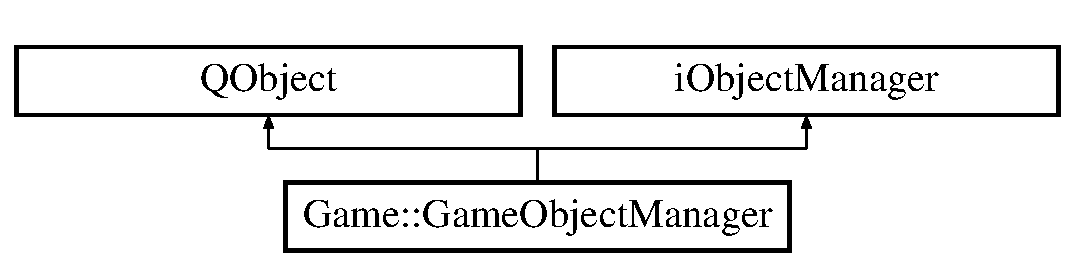
\includegraphics[height=2.000000cm]{class_game_1_1_game_object_manager}
\end{center}
\end{figure}
\subsection*{Public Member Functions}
\begin{DoxyCompactItemize}
\item 
\hyperlink{class_game_1_1_game_object_manager_a6f07c1fc06916333432392170fab4439}{Game\-Object\-Manager} (Q\-Object $\ast$parent=nullptr)
\begin{DoxyCompactList}\small\item\em \hyperlink{class_game_1_1_game_object_manager}{Game\-Object\-Manager}. \end{DoxyCompactList}\item 
void \hyperlink{class_game_1_1_game_object_manager_a616e55e5188f96f3925b7f14f4f9b2f1}{add\-Tiles} (const std\-::vector$<$ std\-::shared\-\_\-ptr$<$ Course\-::\-Tile\-Base $>$$>$ \&tiles)
\begin{DoxyCompactList}\small\item\em add\-Tiles \end{DoxyCompactList}\item 
\hypertarget{class_game_1_1_game_object_manager_abfe2898c4389ca575093917f88e0087b}{void \hyperlink{class_game_1_1_game_object_manager_abfe2898c4389ca575093917f88e0087b}{add\-Game\-Tile} (std\-::shared\-\_\-ptr$<$ \hyperlink{class_game_1_1_game_tile_base}{Game\-::\-Game\-Tile\-Base} $>$ tile)}\label{class_game_1_1_game_object_manager_abfe2898c4389ca575093917f88e0087b}

\begin{DoxyCompactList}\small\item\em add\-Game\-Tile adds tile to gametile-\/vector \end{DoxyCompactList}\item 
\hypertarget{class_game_1_1_game_object_manager_aff2871bd2a6f7daae354da6fee9e1d5d}{std\-::shared\-\_\-ptr$<$ Course\-::\-Tile\-Base $>$ {\bfseries get\-Tile} (const Course\-::\-Coordinate \&coordinate)}\label{class_game_1_1_game_object_manager_aff2871bd2a6f7daae354da6fee9e1d5d}

\item 
std\-::vector$<$ std\-::shared\-\_\-ptr\\*
$<$ Course\-::\-Game\-Object $>$ $>$ \hyperlink{class_game_1_1_game_object_manager_a770203790e7e11185bf53ef1f066cd6c}{get\-Game\-Objects} ()
\begin{DoxyCompactList}\small\item\em get\-Game\-Objects \end{DoxyCompactList}\item 
std\-::shared\-\_\-ptr$<$ Course\-::\-Tile\-Base $>$ \hyperlink{class_game_1_1_game_object_manager_acfcc8a567591bf1bcb3d7a040534383b}{get\-Tile} (const Course\-::\-Object\-Id \&id)
\begin{DoxyCompactList}\small\item\em get\-Tile \end{DoxyCompactList}\item 
std\-::vector$<$ std\-::shared\-\_\-ptr\\*
$<$ Course\-::\-Tile\-Base $>$ $>$ \hyperlink{class_game_1_1_game_object_manager_a2db95d0caf64f0745bfb78d38ab5eb9f}{get\-Tiles} (const std\-::vector$<$ Course\-::\-Coordinate $>$ \&coordinates)
\begin{DoxyCompactList}\small\item\em get\-Tiles \end{DoxyCompactList}\item 
std\-::vector$<$ std\-::shared\-\_\-ptr\\*
$<$ \hyperlink{class_game_1_1_game_tile_base}{Game\-::\-Game\-Tile\-Base} $>$ $>$ \hyperlink{class_game_1_1_game_object_manager_ac600164bb9c69c764aeb0c110a772305}{get\-Game\-Tiles} ()
\begin{DoxyCompactList}\small\item\em get\-Game\-Tiles \end{DoxyCompactList}\item 
\hypertarget{class_game_1_1_game_object_manager_a1b7ed09f5aa0db4be872b580040d2614}{std\-::shared\-\_\-ptr\\*
$<$ \hyperlink{class_game_1_1_game_tile_base}{Game\-::\-Game\-Tile\-Base} $>$ \hyperlink{class_game_1_1_game_object_manager_a1b7ed09f5aa0db4be872b580040d2614}{get\-Game\-Tile} (const Course\-::\-Coordinate \&coordinate)}\label{class_game_1_1_game_object_manager_a1b7ed09f5aa0db4be872b580040d2614}

\begin{DoxyCompactList}\small\item\em get\-Game\-Tile returns the tile in given coordinates \end{DoxyCompactList}\item 
void \hyperlink{class_game_1_1_game_object_manager_a2a3c2db760d5dae0eca50ba1336d111a}{set\-Player} (std\-::shared\-\_\-ptr$<$ \hyperlink{class_game_1_1_player}{Game\-::\-Player} $>$ player)
\begin{DoxyCompactList}\small\item\em set\-Player used from mapgenerator to set player \end{DoxyCompactList}\item 
std\-::shared\-\_\-ptr$<$ \hyperlink{class_game_1_1_player}{Game\-::\-Player} $>$ \hyperlink{class_game_1_1_game_object_manager_a324505448a478a74a4485c7517f2af8d}{get\-Player} ()
\begin{DoxyCompactList}\small\item\em get\-Player used in different classes to get players pointer to get to players attributes \end{DoxyCompactList}\item 
std\-::vector$<$ std\-::shared\-\_\-ptr\\*
$<$ Course\-::\-Worker\-Base $>$ $>$ \hyperlink{class_game_1_1_game_object_manager_a15bafc071007133e9a4c971050b72506}{get\-Workers} ()
\begin{DoxyCompactList}\small\item\em get\-Workers \end{DoxyCompactList}\item 
void \hyperlink{class_game_1_1_game_object_manager_ab5dc0d2150e7df5821b974b12ee4cf54}{add\-Worker} (std\-::shared\-\_\-ptr$<$ Course\-::\-Worker\-Base $>$ worker)
\begin{DoxyCompactList}\small\item\em add\-Worker \end{DoxyCompactList}\item 
void \hyperlink{class_game_1_1_game_object_manager_ae0e1788a3b1b9edf64cda2a259201832}{add\-Game\-Object} (std\-::shared\-\_\-ptr$<$ Course\-::\-Game\-Object $>$ object)
\begin{DoxyCompactList}\small\item\em add\-Game\-Object \end{DoxyCompactList}\item 
void \hyperlink{class_game_1_1_game_object_manager_a0515eff15f2bf07611c2192cf1283fbe}{add\-Building} (std\-::shared\-\_\-ptr$<$ Course\-::\-Building\-Base $>$ building)
\begin{DoxyCompactList}\small\item\em add\-Building \end{DoxyCompactList}\item 
std\-::vector$<$ std\-::shared\-\_\-ptr\\*
$<$ Course\-::\-Building\-Base $>$ $>$ \hyperlink{class_game_1_1_game_object_manager_ad3513f166c73c56409e4abe89bb5d021}{get\-Buildings} ()
\begin{DoxyCompactList}\small\item\em get\-Buildings \end{DoxyCompactList}\end{DoxyCompactItemize}


\subsection{Constructor \& Destructor Documentation}
\hypertarget{class_game_1_1_game_object_manager_a6f07c1fc06916333432392170fab4439}{\index{Game\-::\-Game\-Object\-Manager@{Game\-::\-Game\-Object\-Manager}!Game\-Object\-Manager@{Game\-Object\-Manager}}
\index{Game\-Object\-Manager@{Game\-Object\-Manager}!Game::GameObjectManager@{Game\-::\-Game\-Object\-Manager}}
\subsubsection[{Game\-Object\-Manager}]{\setlength{\rightskip}{0pt plus 5cm}Game\-::\-Game\-Object\-Manager\-::\-Game\-Object\-Manager (
\begin{DoxyParamCaption}
\item[{Q\-Object $\ast$}]{parent = {\ttfamily nullptr}}
\end{DoxyParamCaption}
)}}\label{class_game_1_1_game_object_manager_a6f07c1fc06916333432392170fab4439}


\hyperlink{class_game_1_1_game_object_manager}{Game\-Object\-Manager}. 


\begin{DoxyParams}{Parameters}
{\em parent} & \\
\hline
\end{DoxyParams}


\subsection{Member Function Documentation}
\hypertarget{class_game_1_1_game_object_manager_a0515eff15f2bf07611c2192cf1283fbe}{\index{Game\-::\-Game\-Object\-Manager@{Game\-::\-Game\-Object\-Manager}!add\-Building@{add\-Building}}
\index{add\-Building@{add\-Building}!Game::GameObjectManager@{Game\-::\-Game\-Object\-Manager}}
\subsubsection[{add\-Building}]{\setlength{\rightskip}{0pt plus 5cm}void Game\-::\-Game\-Object\-Manager\-::add\-Building (
\begin{DoxyParamCaption}
\item[{std\-::shared\-\_\-ptr$<$ Course\-::\-Building\-Base $>$}]{building}
\end{DoxyParamCaption}
)}}\label{class_game_1_1_game_object_manager_a0515eff15f2bf07611c2192cf1283fbe}


add\-Building 


\begin{DoxyParams}{Parameters}
{\em building} & stores a builkding in the object manager \\
\hline
\end{DoxyParams}
\hypertarget{class_game_1_1_game_object_manager_ae0e1788a3b1b9edf64cda2a259201832}{\index{Game\-::\-Game\-Object\-Manager@{Game\-::\-Game\-Object\-Manager}!add\-Game\-Object@{add\-Game\-Object}}
\index{add\-Game\-Object@{add\-Game\-Object}!Game::GameObjectManager@{Game\-::\-Game\-Object\-Manager}}
\subsubsection[{add\-Game\-Object}]{\setlength{\rightskip}{0pt plus 5cm}void Game\-::\-Game\-Object\-Manager\-::add\-Game\-Object (
\begin{DoxyParamCaption}
\item[{std\-::shared\-\_\-ptr$<$ Course\-::\-Game\-Object $>$}]{object}
\end{DoxyParamCaption}
)}}\label{class_game_1_1_game_object_manager_ae0e1788a3b1b9edf64cda2a259201832}


add\-Game\-Object 


\begin{DoxyParams}{Parameters}
{\em object} & stores a game object in the object manager \\
\hline
\end{DoxyParams}
\hypertarget{class_game_1_1_game_object_manager_a616e55e5188f96f3925b7f14f4f9b2f1}{\index{Game\-::\-Game\-Object\-Manager@{Game\-::\-Game\-Object\-Manager}!add\-Tiles@{add\-Tiles}}
\index{add\-Tiles@{add\-Tiles}!Game::GameObjectManager@{Game\-::\-Game\-Object\-Manager}}
\subsubsection[{add\-Tiles}]{\setlength{\rightskip}{0pt plus 5cm}void Game\-::\-Game\-Object\-Manager\-::add\-Tiles (
\begin{DoxyParamCaption}
\item[{const std\-::vector$<$ std\-::shared\-\_\-ptr$<$ Course\-::\-Tile\-Base $>$$>$ \&}]{tiles}
\end{DoxyParamCaption}
)}}\label{class_game_1_1_game_object_manager_a616e55e5188f96f3925b7f14f4f9b2f1}


add\-Tiles 


\begin{DoxyParams}{Parameters}
{\em tiles} & stores a vector of tiles into the object manager \\
\hline
\end{DoxyParams}
\hypertarget{class_game_1_1_game_object_manager_ab5dc0d2150e7df5821b974b12ee4cf54}{\index{Game\-::\-Game\-Object\-Manager@{Game\-::\-Game\-Object\-Manager}!add\-Worker@{add\-Worker}}
\index{add\-Worker@{add\-Worker}!Game::GameObjectManager@{Game\-::\-Game\-Object\-Manager}}
\subsubsection[{add\-Worker}]{\setlength{\rightskip}{0pt plus 5cm}void Game\-::\-Game\-Object\-Manager\-::add\-Worker (
\begin{DoxyParamCaption}
\item[{std\-::shared\-\_\-ptr$<$ Course\-::\-Worker\-Base $>$}]{worker}
\end{DoxyParamCaption}
)}}\label{class_game_1_1_game_object_manager_ab5dc0d2150e7df5821b974b12ee4cf54}


add\-Worker 


\begin{DoxyParams}{Parameters}
{\em worker} & stores a worker in the object manager \\
\hline
\end{DoxyParams}
\hypertarget{class_game_1_1_game_object_manager_ad3513f166c73c56409e4abe89bb5d021}{\index{Game\-::\-Game\-Object\-Manager@{Game\-::\-Game\-Object\-Manager}!get\-Buildings@{get\-Buildings}}
\index{get\-Buildings@{get\-Buildings}!Game::GameObjectManager@{Game\-::\-Game\-Object\-Manager}}
\subsubsection[{get\-Buildings}]{\setlength{\rightskip}{0pt plus 5cm}std\-::vector$<$ std\-::shared\-\_\-ptr$<$ Course\-::\-Building\-Base $>$ $>$ Game\-::\-Game\-Object\-Manager\-::get\-Buildings (
\begin{DoxyParamCaption}
{}
\end{DoxyParamCaption}
)}}\label{class_game_1_1_game_object_manager_ad3513f166c73c56409e4abe89bb5d021}


get\-Buildings 

\begin{DoxyReturn}{Returns}
vector of buildings returns all the buildings that have been stored 
\end{DoxyReturn}
\hypertarget{class_game_1_1_game_object_manager_a770203790e7e11185bf53ef1f066cd6c}{\index{Game\-::\-Game\-Object\-Manager@{Game\-::\-Game\-Object\-Manager}!get\-Game\-Objects@{get\-Game\-Objects}}
\index{get\-Game\-Objects@{get\-Game\-Objects}!Game::GameObjectManager@{Game\-::\-Game\-Object\-Manager}}
\subsubsection[{get\-Game\-Objects}]{\setlength{\rightskip}{0pt plus 5cm}std\-::vector$<$ std\-::shared\-\_\-ptr$<$ Course\-::\-Game\-Object $>$ $>$ Game\-::\-Game\-Object\-Manager\-::get\-Game\-Objects (
\begin{DoxyParamCaption}
{}
\end{DoxyParamCaption}
)}}\label{class_game_1_1_game_object_manager_a770203790e7e11185bf53ef1f066cd6c}


get\-Game\-Objects 

\begin{DoxyReturn}{Returns}
vector containing all gameobjects 
\end{DoxyReturn}
\hypertarget{class_game_1_1_game_object_manager_ac600164bb9c69c764aeb0c110a772305}{\index{Game\-::\-Game\-Object\-Manager@{Game\-::\-Game\-Object\-Manager}!get\-Game\-Tiles@{get\-Game\-Tiles}}
\index{get\-Game\-Tiles@{get\-Game\-Tiles}!Game::GameObjectManager@{Game\-::\-Game\-Object\-Manager}}
\subsubsection[{get\-Game\-Tiles}]{\setlength{\rightskip}{0pt plus 5cm}std\-::vector$<$ std\-::shared\-\_\-ptr$<$ {\bf Game\-Tile\-Base} $>$ $>$ Game\-::\-Game\-Object\-Manager\-::get\-Game\-Tiles (
\begin{DoxyParamCaption}
{}
\end{DoxyParamCaption}
)}}\label{class_game_1_1_game_object_manager_ac600164bb9c69c764aeb0c110a772305}


get\-Game\-Tiles 

\begin{DoxyReturn}{Returns}
returns vector containing all gametiles 
\end{DoxyReturn}
\hypertarget{class_game_1_1_game_object_manager_a324505448a478a74a4485c7517f2af8d}{\index{Game\-::\-Game\-Object\-Manager@{Game\-::\-Game\-Object\-Manager}!get\-Player@{get\-Player}}
\index{get\-Player@{get\-Player}!Game::GameObjectManager@{Game\-::\-Game\-Object\-Manager}}
\subsubsection[{get\-Player}]{\setlength{\rightskip}{0pt plus 5cm}std\-::shared\-\_\-ptr$<$ {\bf Player} $>$ Game\-::\-Game\-Object\-Manager\-::get\-Player (
\begin{DoxyParamCaption}
{}
\end{DoxyParamCaption}
)}}\label{class_game_1_1_game_object_manager_a324505448a478a74a4485c7517f2af8d}


get\-Player used in different classes to get players pointer to get to players attributes 

\begin{DoxyReturn}{Returns}
pointer to player 
\end{DoxyReturn}
\hypertarget{class_game_1_1_game_object_manager_acfcc8a567591bf1bcb3d7a040534383b}{\index{Game\-::\-Game\-Object\-Manager@{Game\-::\-Game\-Object\-Manager}!get\-Tile@{get\-Tile}}
\index{get\-Tile@{get\-Tile}!Game::GameObjectManager@{Game\-::\-Game\-Object\-Manager}}
\subsubsection[{get\-Tile}]{\setlength{\rightskip}{0pt plus 5cm}std\-::shared\-\_\-ptr$<$ Course\-::\-Tile\-Base $>$ Game\-::\-Game\-Object\-Manager\-::get\-Tile (
\begin{DoxyParamCaption}
\item[{const Course\-::\-Object\-Id \&}]{id}
\end{DoxyParamCaption}
)}}\label{class_game_1_1_game_object_manager_acfcc8a567591bf1bcb3d7a040534383b}


get\-Tile 


\begin{DoxyParams}{Parameters}
{\em id} & \\
\hline
\end{DoxyParams}
\begin{DoxyReturn}{Returns}
shared pointer that points to the tile that has the given I\-D Use to get a tile with a certain I\-D 
\end{DoxyReturn}
\hypertarget{class_game_1_1_game_object_manager_a2db95d0caf64f0745bfb78d38ab5eb9f}{\index{Game\-::\-Game\-Object\-Manager@{Game\-::\-Game\-Object\-Manager}!get\-Tiles@{get\-Tiles}}
\index{get\-Tiles@{get\-Tiles}!Game::GameObjectManager@{Game\-::\-Game\-Object\-Manager}}
\subsubsection[{get\-Tiles}]{\setlength{\rightskip}{0pt plus 5cm}std\-::vector$<$ std\-::shared\-\_\-ptr$<$ Course\-::\-Tile\-Base $>$ $>$ Game\-::\-Game\-Object\-Manager\-::get\-Tiles (
\begin{DoxyParamCaption}
\item[{const std\-::vector$<$ Course\-::\-Coordinate $>$ \&}]{coordinates}
\end{DoxyParamCaption}
)}}\label{class_game_1_1_game_object_manager_a2db95d0caf64f0745bfb78d38ab5eb9f}


get\-Tiles 


\begin{DoxyParams}{Parameters}
{\em coordinates} & \\
\hline
\end{DoxyParams}
\begin{DoxyReturn}{Returns}
vector of shared pointers that point to the tiles with given coordinates Use to get the tiles in an area or multiple locations 
\end{DoxyReturn}
\hypertarget{class_game_1_1_game_object_manager_a15bafc071007133e9a4c971050b72506}{\index{Game\-::\-Game\-Object\-Manager@{Game\-::\-Game\-Object\-Manager}!get\-Workers@{get\-Workers}}
\index{get\-Workers@{get\-Workers}!Game::GameObjectManager@{Game\-::\-Game\-Object\-Manager}}
\subsubsection[{get\-Workers}]{\setlength{\rightskip}{0pt plus 5cm}std\-::vector$<$ std\-::shared\-\_\-ptr$<$ Course\-::\-Worker\-Base $>$ $>$ Game\-::\-Game\-Object\-Manager\-::get\-Workers (
\begin{DoxyParamCaption}
{}
\end{DoxyParamCaption}
)}}\label{class_game_1_1_game_object_manager_a15bafc071007133e9a4c971050b72506}


get\-Workers 

\begin{DoxyReturn}{Returns}
vector with all the workers 
\end{DoxyReturn}
\hypertarget{class_game_1_1_game_object_manager_a2a3c2db760d5dae0eca50ba1336d111a}{\index{Game\-::\-Game\-Object\-Manager@{Game\-::\-Game\-Object\-Manager}!set\-Player@{set\-Player}}
\index{set\-Player@{set\-Player}!Game::GameObjectManager@{Game\-::\-Game\-Object\-Manager}}
\subsubsection[{set\-Player}]{\setlength{\rightskip}{0pt plus 5cm}void Game\-::\-Game\-Object\-Manager\-::set\-Player (
\begin{DoxyParamCaption}
\item[{std\-::shared\-\_\-ptr$<$ {\bf Game\-::\-Player} $>$}]{player}
\end{DoxyParamCaption}
)}}\label{class_game_1_1_game_object_manager_a2a3c2db760d5dae0eca50ba1336d111a}


set\-Player used from mapgenerator to set player 


\begin{DoxyParams}{Parameters}
{\em player} & \\
\hline
\end{DoxyParams}


The documentation for this class was generated from the following files\-:\begin{DoxyCompactItemize}
\item 
gameobjectmanager.\-h\item 
gameobjectmanager.\-cpp\end{DoxyCompactItemize}

\hypertarget{class_game_1_1_game_tile_base}{\section{Game\-:\-:Game\-Tile\-Base Class Reference}
\label{class_game_1_1_game_tile_base}\index{Game\-::\-Game\-Tile\-Base@{Game\-::\-Game\-Tile\-Base}}
}


The \hyperlink{class_game_1_1_game_tile_base}{Game\-Tile\-Base} class base class for all tiles used in game.  




{\ttfamily \#include $<$gametilebase.\-h$>$}

Inheritance diagram for Game\-:\-:Game\-Tile\-Base\-:\begin{figure}[H]
\begin{center}
\leavevmode
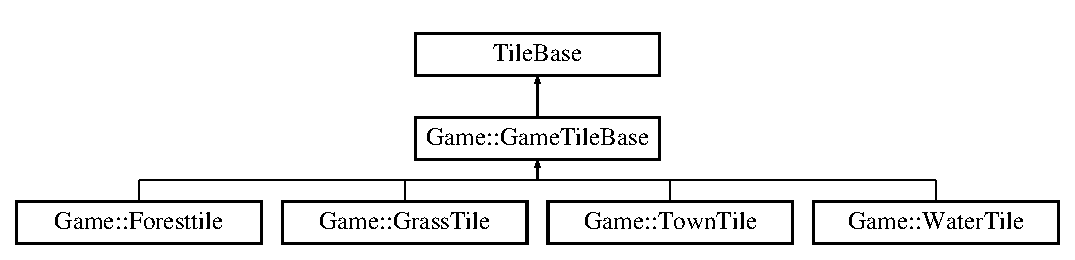
\includegraphics[height=3.000000cm]{class_game_1_1_game_tile_base}
\end{center}
\end{figure}
\subsection*{Public Member Functions}
\begin{DoxyCompactItemize}
\item 
\hyperlink{class_game_1_1_game_tile_base_ac89ced36f5a5c6a9c598a59e0a9bde9f}{Game\-Tile\-Base} (const Course\-::\-Coordinate \&location, const std\-::shared\-\_\-ptr$<$ \hyperlink{class_game_1_1_game_event_handler}{Game\-Event\-Handler} $>$ \&eventhandler, const std\-::shared\-\_\-ptr$<$ \hyperlink{class_game_1_1_game_object_manager}{Game\-Object\-Manager} $>$ \&objectmanager, const unsigned int \&max\-\_\-build=1, const unsigned int \&max\-\_\-work=3, const Course\-::\-Resource\-Map \&production=Game\-::\-Const\-Game\-Resource\-Map\-::\-T\-I\-L\-E\-\_\-\-B\-P)
\begin{DoxyCompactList}\small\item\em \hyperlink{class_game_1_1_game_tile_base}{Game\-Tile\-Base}. \end{DoxyCompactList}\item 
virtual Q\-Pixmap \hyperlink{class_game_1_1_game_tile_base_a88170bec69ba095ca6ffeea469532bff}{get\-Sprite} ()
\begin{DoxyCompactList}\small\item\em get\-Sprite \end{DoxyCompactList}\item 
void \hyperlink{class_game_1_1_game_tile_base_a4c986a263864df783c280cc127b595d3}{update\-Sprite} (Q\-Pixmap new\-Sprite)
\begin{DoxyCompactList}\small\item\em update\-Sprite \end{DoxyCompactList}\item 
bool \hyperlink{class_game_1_1_game_tile_base_a180c056c094375ecad334dadc1413608}{get\-Robber} ()
\begin{DoxyCompactList}\small\item\em get\-Robber \end{DoxyCompactList}\item 
bool \hyperlink{class_game_1_1_game_tile_base_aa20e5ba9b5ba81a4d72786aa0f05495e}{get\-Treasure} ()
\begin{DoxyCompactList}\small\item\em get\-Treasure \end{DoxyCompactList}\item 
int \hyperlink{class_game_1_1_game_tile_base_a65cb55e1e7de1c0c3b8cbf770d8e325c}{get\-Height} ()
\begin{DoxyCompactList}\small\item\em get\-Height \end{DoxyCompactList}\item 
int \hyperlink{class_game_1_1_game_tile_base_a0b02032614ded5bc23ed81bd81cef6cf}{get\-Width} ()
\begin{DoxyCompactList}\small\item\em get\-Width \end{DoxyCompactList}\item 
void \hyperlink{class_game_1_1_game_tile_base_a0be2dfb1431a55bce1f84b29645ae932}{set\-Robber} (bool robber)
\begin{DoxyCompactList}\small\item\em set\-Robber if robber == true, tile will have a robber \end{DoxyCompactList}\item 
void \hyperlink{class_game_1_1_game_tile_base_a2bc4d0458c01992cc5a975d119765551}{set\-Treasure} (bool treasure)
\begin{DoxyCompactList}\small\item\em set\-Treasure if treasure == true, tile will have a trasure \end{DoxyCompactList}\end{DoxyCompactItemize}
\subsection*{Protected Attributes}
\begin{DoxyCompactItemize}
\item 
\hypertarget{class_game_1_1_game_tile_base_a2d72336befccee4083acae3e36bbc40e}{Q\-Pixmap {\bfseries sprite}}\label{class_game_1_1_game_tile_base_a2d72336befccee4083acae3e36bbc40e}

\item 
\hypertarget{class_game_1_1_game_tile_base_a64279e63a53c5a9d8f44e50493eac9c6}{bool {\bfseries has\-Robber}}\label{class_game_1_1_game_tile_base_a64279e63a53c5a9d8f44e50493eac9c6}

\item 
\hypertarget{class_game_1_1_game_tile_base_a5ddf32ac3c7cda213c767879a12d5610}{bool {\bfseries has\-Treasure}}\label{class_game_1_1_game_tile_base_a5ddf32ac3c7cda213c767879a12d5610}

\item 
\hypertarget{class_game_1_1_game_tile_base_ad939859fa92994f157d7728b60b3dbff}{int {\bfseries treasure}}\label{class_game_1_1_game_tile_base_ad939859fa92994f157d7728b60b3dbff}

\item 
\hypertarget{class_game_1_1_game_tile_base_ad0ee0109c45a8091f2bc202d4a4ab0ff}{int {\bfseries width}}\label{class_game_1_1_game_tile_base_ad0ee0109c45a8091f2bc202d4a4ab0ff}

\item 
\hypertarget{class_game_1_1_game_tile_base_aef220c70f71d82800229b071e52689a3}{int {\bfseries height}}\label{class_game_1_1_game_tile_base_aef220c70f71d82800229b071e52689a3}

\end{DoxyCompactItemize}


\subsection{Detailed Description}
The \hyperlink{class_game_1_1_game_tile_base}{Game\-Tile\-Base} class base class for all tiles used in game. 

\subsection{Constructor \& Destructor Documentation}
\hypertarget{class_game_1_1_game_tile_base_ac89ced36f5a5c6a9c598a59e0a9bde9f}{\index{Game\-::\-Game\-Tile\-Base@{Game\-::\-Game\-Tile\-Base}!Game\-Tile\-Base@{Game\-Tile\-Base}}
\index{Game\-Tile\-Base@{Game\-Tile\-Base}!Game::GameTileBase@{Game\-::\-Game\-Tile\-Base}}
\subsubsection[{Game\-Tile\-Base}]{\setlength{\rightskip}{0pt plus 5cm}Game\-::\-Game\-Tile\-Base\-::\-Game\-Tile\-Base (
\begin{DoxyParamCaption}
\item[{const Course\-::\-Coordinate \&}]{location, }
\item[{const std\-::shared\-\_\-ptr$<$ {\bf Game\-Event\-Handler} $>$ \&}]{eventhandler, }
\item[{const std\-::shared\-\_\-ptr$<$ {\bf Game\-Object\-Manager} $>$ \&}]{objectmanager, }
\item[{const unsigned int \&}]{max\-\_\-build = {\ttfamily 1}, }
\item[{const unsigned int \&}]{max\-\_\-work = {\ttfamily 3}, }
\item[{const Course\-::\-Resource\-Map \&}]{production = {\ttfamily Game\-:\-:ConstGameResourceMap\-:\-:TILE\-\_\-BP}}
\end{DoxyParamCaption}
)}}\label{class_game_1_1_game_tile_base_ac89ced36f5a5c6a9c598a59e0a9bde9f}


\hyperlink{class_game_1_1_game_tile_base}{Game\-Tile\-Base}. 


\begin{DoxyParams}{Parameters}
{\em location} & \\
\hline
{\em eventhandler} & \\
\hline
{\em objectmanager} & \\
\hline
{\em max\-\_\-build} & maximum amount of buildings that can be placed on the tile \\
\hline
{\em max\-\_\-work} & maximum amount of workers that can be placed on the tile \\
\hline
{\em production} & \\
\hline
\end{DoxyParams}


\subsection{Member Function Documentation}
\hypertarget{class_game_1_1_game_tile_base_a65cb55e1e7de1c0c3b8cbf770d8e325c}{\index{Game\-::\-Game\-Tile\-Base@{Game\-::\-Game\-Tile\-Base}!get\-Height@{get\-Height}}
\index{get\-Height@{get\-Height}!Game::GameTileBase@{Game\-::\-Game\-Tile\-Base}}
\subsubsection[{get\-Height}]{\setlength{\rightskip}{0pt plus 5cm}int Game\-::\-Game\-Tile\-Base\-::get\-Height (
\begin{DoxyParamCaption}
{}
\end{DoxyParamCaption}
)}}\label{class_game_1_1_game_tile_base_a65cb55e1e7de1c0c3b8cbf770d8e325c}


get\-Height 

\begin{DoxyReturn}{Returns}
height of the sprite image 
\end{DoxyReturn}
\hypertarget{class_game_1_1_game_tile_base_a180c056c094375ecad334dadc1413608}{\index{Game\-::\-Game\-Tile\-Base@{Game\-::\-Game\-Tile\-Base}!get\-Robber@{get\-Robber}}
\index{get\-Robber@{get\-Robber}!Game::GameTileBase@{Game\-::\-Game\-Tile\-Base}}
\subsubsection[{get\-Robber}]{\setlength{\rightskip}{0pt plus 5cm}bool Game\-::\-Game\-Tile\-Base\-::get\-Robber (
\begin{DoxyParamCaption}
{}
\end{DoxyParamCaption}
)}}\label{class_game_1_1_game_tile_base_a180c056c094375ecad334dadc1413608}


get\-Robber 

\begin{DoxyReturn}{Returns}
true, if tile has robber, false if not 
\end{DoxyReturn}
\hypertarget{class_game_1_1_game_tile_base_a88170bec69ba095ca6ffeea469532bff}{\index{Game\-::\-Game\-Tile\-Base@{Game\-::\-Game\-Tile\-Base}!get\-Sprite@{get\-Sprite}}
\index{get\-Sprite@{get\-Sprite}!Game::GameTileBase@{Game\-::\-Game\-Tile\-Base}}
\subsubsection[{get\-Sprite}]{\setlength{\rightskip}{0pt plus 5cm}Q\-Pixmap Game\-::\-Game\-Tile\-Base\-::get\-Sprite (
\begin{DoxyParamCaption}
{}
\end{DoxyParamCaption}
)\hspace{0.3cm}{\ttfamily [virtual]}}}\label{class_game_1_1_game_tile_base_a88170bec69ba095ca6ffeea469532bff}


get\-Sprite 

\begin{DoxyReturn}{Returns}
Qpixmap image to draw buildings to map scene 
\end{DoxyReturn}
\hypertarget{class_game_1_1_game_tile_base_aa20e5ba9b5ba81a4d72786aa0f05495e}{\index{Game\-::\-Game\-Tile\-Base@{Game\-::\-Game\-Tile\-Base}!get\-Treasure@{get\-Treasure}}
\index{get\-Treasure@{get\-Treasure}!Game::GameTileBase@{Game\-::\-Game\-Tile\-Base}}
\subsubsection[{get\-Treasure}]{\setlength{\rightskip}{0pt plus 5cm}bool Game\-::\-Game\-Tile\-Base\-::get\-Treasure (
\begin{DoxyParamCaption}
{}
\end{DoxyParamCaption}
)}}\label{class_game_1_1_game_tile_base_aa20e5ba9b5ba81a4d72786aa0f05495e}


get\-Treasure 

\begin{DoxyReturn}{Returns}
true, if tile has treasure, false if not 
\end{DoxyReturn}
\hypertarget{class_game_1_1_game_tile_base_a0b02032614ded5bc23ed81bd81cef6cf}{\index{Game\-::\-Game\-Tile\-Base@{Game\-::\-Game\-Tile\-Base}!get\-Width@{get\-Width}}
\index{get\-Width@{get\-Width}!Game::GameTileBase@{Game\-::\-Game\-Tile\-Base}}
\subsubsection[{get\-Width}]{\setlength{\rightskip}{0pt plus 5cm}int Game\-::\-Game\-Tile\-Base\-::get\-Width (
\begin{DoxyParamCaption}
{}
\end{DoxyParamCaption}
)}}\label{class_game_1_1_game_tile_base_a0b02032614ded5bc23ed81bd81cef6cf}


get\-Width 

\begin{DoxyReturn}{Returns}
width of the sprite image 
\end{DoxyReturn}
\hypertarget{class_game_1_1_game_tile_base_a0be2dfb1431a55bce1f84b29645ae932}{\index{Game\-::\-Game\-Tile\-Base@{Game\-::\-Game\-Tile\-Base}!set\-Robber@{set\-Robber}}
\index{set\-Robber@{set\-Robber}!Game::GameTileBase@{Game\-::\-Game\-Tile\-Base}}
\subsubsection[{set\-Robber}]{\setlength{\rightskip}{0pt plus 5cm}void Game\-::\-Game\-Tile\-Base\-::set\-Robber (
\begin{DoxyParamCaption}
\item[{bool}]{robber}
\end{DoxyParamCaption}
)}}\label{class_game_1_1_game_tile_base_a0be2dfb1431a55bce1f84b29645ae932}


set\-Robber if robber == true, tile will have a robber 


\begin{DoxyParams}{Parameters}
{\em robber} & \\
\hline
\end{DoxyParams}
\begin{DoxyReturn}{Returns}

\end{DoxyReturn}
\hypertarget{class_game_1_1_game_tile_base_a2bc4d0458c01992cc5a975d119765551}{\index{Game\-::\-Game\-Tile\-Base@{Game\-::\-Game\-Tile\-Base}!set\-Treasure@{set\-Treasure}}
\index{set\-Treasure@{set\-Treasure}!Game::GameTileBase@{Game\-::\-Game\-Tile\-Base}}
\subsubsection[{set\-Treasure}]{\setlength{\rightskip}{0pt plus 5cm}void Game\-::\-Game\-Tile\-Base\-::set\-Treasure (
\begin{DoxyParamCaption}
\item[{bool}]{treasure}
\end{DoxyParamCaption}
)}}\label{class_game_1_1_game_tile_base_a2bc4d0458c01992cc5a975d119765551}


set\-Treasure if treasure == true, tile will have a trasure 


\begin{DoxyParams}{Parameters}
{\em treasure} & \\
\hline
\end{DoxyParams}
\begin{DoxyReturn}{Returns}

\end{DoxyReturn}
\hypertarget{class_game_1_1_game_tile_base_a4c986a263864df783c280cc127b595d3}{\index{Game\-::\-Game\-Tile\-Base@{Game\-::\-Game\-Tile\-Base}!update\-Sprite@{update\-Sprite}}
\index{update\-Sprite@{update\-Sprite}!Game::GameTileBase@{Game\-::\-Game\-Tile\-Base}}
\subsubsection[{update\-Sprite}]{\setlength{\rightskip}{0pt plus 5cm}void Game\-::\-Game\-Tile\-Base\-::update\-Sprite (
\begin{DoxyParamCaption}
\item[{Q\-Pixmap}]{new\-Sprite}
\end{DoxyParamCaption}
)}}\label{class_game_1_1_game_tile_base_a4c986a263864df783c280cc127b595d3}


update\-Sprite 


\begin{DoxyParams}{Parameters}
{\em new\-Sprite} & sets the sprite image to the given one \\
\hline
\end{DoxyParams}


The documentation for this class was generated from the following files\-:\begin{DoxyCompactItemize}
\item 
gametilebase.\-h\item 
gametilebase.\-cpp\end{DoxyCompactItemize}

\hypertarget{class_game_1_1_grass_tile}{\section{Game\-:\-:Grass\-Tile Class Reference}
\label{class_game_1_1_grass_tile}\index{Game\-::\-Grass\-Tile@{Game\-::\-Grass\-Tile}}
}


The \hyperlink{class_game_1_1_grass_tile}{Grass\-Tile} class represents grass.  




{\ttfamily \#include $<$grasstile.\-h$>$}

Inheritance diagram for Game\-:\-:Grass\-Tile\-:\begin{figure}[H]
\begin{center}
\leavevmode
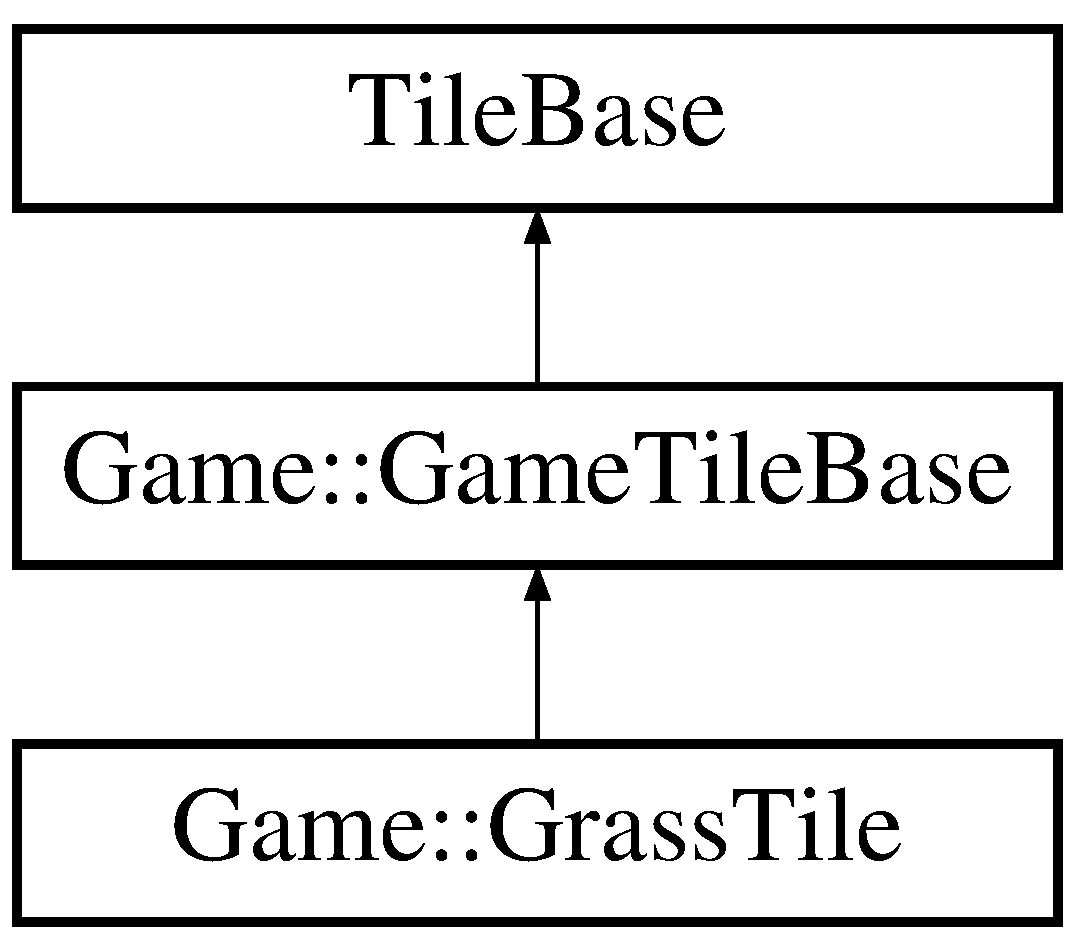
\includegraphics[height=3.000000cm]{class_game_1_1_grass_tile}
\end{center}
\end{figure}
\subsection*{Public Member Functions}
\begin{DoxyCompactItemize}
\item 
\hyperlink{class_game_1_1_grass_tile_ae24ddbbcf79256432c521b6ebcf7deee}{Grass\-Tile} (const Course\-::\-Coordinate \&location, const std\-::shared\-\_\-ptr$<$ \hyperlink{class_game_1_1_game_event_handler}{Game\-Event\-Handler} $>$ \&eventhandler, const std\-::shared\-\_\-ptr$<$ \hyperlink{class_game_1_1_game_object_manager}{Game\-Object\-Manager} $>$ \&objectmanager, const unsigned int \&max\-\_\-build=1, const unsigned int \&max\-\_\-work=3, const Course\-::\-Resource\-Map \&production=Game\-::\-Const\-Game\-Resource\-Map\-::\-T\-I\-L\-E\-\_\-\-B\-P)
\begin{DoxyCompactList}\small\item\em \hyperlink{class_game_1_1_grass_tile}{Grass\-Tile}. \end{DoxyCompactList}\item 
virtual std\-::string \hyperlink{class_game_1_1_grass_tile_aeea563297cc6ed020eda6c252e906e1d}{get\-Type} () const override
\begin{DoxyCompactList}\small\item\em get\-Type \end{DoxyCompactList}\end{DoxyCompactItemize}
\subsection*{Additional Inherited Members}


\subsection{Detailed Description}
The \hyperlink{class_game_1_1_grass_tile}{Grass\-Tile} class represents grass. 

\subsection{Constructor \& Destructor Documentation}
\hypertarget{class_game_1_1_grass_tile_ae24ddbbcf79256432c521b6ebcf7deee}{\index{Game\-::\-Grass\-Tile@{Game\-::\-Grass\-Tile}!Grass\-Tile@{Grass\-Tile}}
\index{Grass\-Tile@{Grass\-Tile}!Game::GrassTile@{Game\-::\-Grass\-Tile}}
\subsubsection[{Grass\-Tile}]{\setlength{\rightskip}{0pt plus 5cm}Game\-::\-Grass\-Tile\-::\-Grass\-Tile (
\begin{DoxyParamCaption}
\item[{const Course\-::\-Coordinate \&}]{location, }
\item[{const std\-::shared\-\_\-ptr$<$ {\bf Game\-Event\-Handler} $>$ \&}]{eventhandler, }
\item[{const std\-::shared\-\_\-ptr$<$ {\bf Game\-Object\-Manager} $>$ \&}]{objectmanager, }
\item[{const unsigned int \&}]{max\-\_\-build = {\ttfamily 1}, }
\item[{const unsigned int \&}]{max\-\_\-work = {\ttfamily 3}, }
\item[{const Course\-::\-Resource\-Map \&}]{production = {\ttfamily Game\-:\-:ConstGameResourceMap\-:\-:TILE\-\_\-BP}}
\end{DoxyParamCaption}
)}}\label{class_game_1_1_grass_tile_ae24ddbbcf79256432c521b6ebcf7deee}


\hyperlink{class_game_1_1_grass_tile}{Grass\-Tile}. 


\begin{DoxyParams}{Parameters}
{\em location} & \\
\hline
{\em eventhandler} & \\
\hline
{\em objectmanager} & \\
\hline
{\em max\-\_\-build} & \\
\hline
{\em max\-\_\-work} & \\
\hline
{\em production} & \\
\hline
\end{DoxyParams}


\subsection{Member Function Documentation}
\hypertarget{class_game_1_1_grass_tile_aeea563297cc6ed020eda6c252e906e1d}{\index{Game\-::\-Grass\-Tile@{Game\-::\-Grass\-Tile}!get\-Type@{get\-Type}}
\index{get\-Type@{get\-Type}!Game::GrassTile@{Game\-::\-Grass\-Tile}}
\subsubsection[{get\-Type}]{\setlength{\rightskip}{0pt plus 5cm}std\-::string Game\-::\-Grass\-Tile\-::get\-Type (
\begin{DoxyParamCaption}
{}
\end{DoxyParamCaption}
) const\hspace{0.3cm}{\ttfamily [override]}, {\ttfamily [virtual]}}}\label{class_game_1_1_grass_tile_aeea563297cc6ed020eda6c252e906e1d}


get\-Type 

\begin{DoxyReturn}{Returns}
type of the tile as a string 
\end{DoxyReturn}


The documentation for this class was generated from the following files\-:\begin{DoxyCompactItemize}
\item 
Tiles/grasstile.\-h\item 
Tiles/grasstile.\-cpp\end{DoxyCompactItemize}

\hypertarget{class_game_1_1_logging_building}{\section{Game\-:\-:Logging\-Building Class Reference}
\label{class_game_1_1_logging_building}\index{Game\-::\-Logging\-Building@{Game\-::\-Logging\-Building}}
}


The \hyperlink{class_game_1_1_logging_building}{Logging\-Building} class represents a logging cabin.  




{\ttfamily \#include $<$loggingbuilding.\-h$>$}

Inheritance diagram for Game\-:\-:Logging\-Building\-:\begin{figure}[H]
\begin{center}
\leavevmode
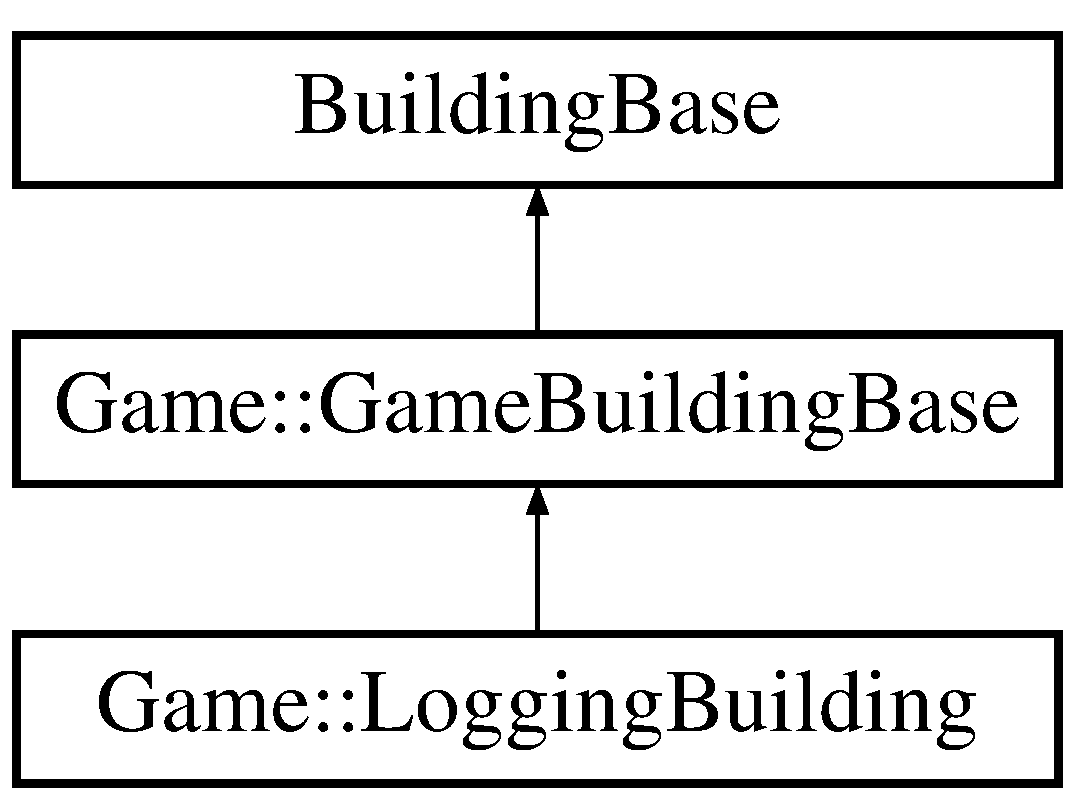
\includegraphics[height=3.000000cm]{class_game_1_1_logging_building}
\end{center}
\end{figure}
\subsection*{Public Member Functions}
\begin{DoxyCompactItemize}
\item 
\hyperlink{class_game_1_1_logging_building_a207f9472b3a0df5853a37b03bd84a937}{Logging\-Building} (const std\-::shared\-\_\-ptr$<$ \hyperlink{class_game_1_1_game_event_handler}{Game\-Event\-Handler} $>$ \&eventhandler, const std\-::shared\-\_\-ptr$<$ \hyperlink{class_game_1_1_game_object_manager}{Game\-Object\-Manager} $>$ \&objectmanager, const std\-::shared\-\_\-ptr$<$ \hyperlink{class_game_1_1_player}{Game\-::\-Player} $>$ \&owner, const int \&tilespaces=1, const Course\-::\-Resource\-Map \&buildcost=Game\-::\-Const\-Game\-Resource\-Map\-::\-L\-O\-G\-G\-I\-N\-G\-\_\-\-B\-U\-I\-L\-D\-\_\-\-C\-O\-S\-T, const Course\-::\-Resource\-Map \&production=Game\-::\-Const\-Game\-Resource\-Map\-::\-L\-O\-G\-G\-I\-N\-G\-\_\-\-P\-R\-O\-D\-U\-C\-T\-I\-O\-N)
\begin{DoxyCompactList}\small\item\em \hyperlink{class_game_1_1_logging_building}{Logging\-Building}. \end{DoxyCompactList}\item 
virtual std\-::string \hyperlink{class_game_1_1_logging_building_a052eb3f8b6496e0b9028d7f3281f9f9c}{get\-Type} () const override
\begin{DoxyCompactList}\small\item\em get\-Type \end{DoxyCompactList}\end{DoxyCompactItemize}
\subsection*{Additional Inherited Members}


\subsection{Detailed Description}
The \hyperlink{class_game_1_1_logging_building}{Logging\-Building} class represents a logging cabin. 

\subsection{Constructor \& Destructor Documentation}
\hypertarget{class_game_1_1_logging_building_a207f9472b3a0df5853a37b03bd84a937}{\index{Game\-::\-Logging\-Building@{Game\-::\-Logging\-Building}!Logging\-Building@{Logging\-Building}}
\index{Logging\-Building@{Logging\-Building}!Game::LoggingBuilding@{Game\-::\-Logging\-Building}}
\subsubsection[{Logging\-Building}]{\setlength{\rightskip}{0pt plus 5cm}Game\-::\-Logging\-Building\-::\-Logging\-Building (
\begin{DoxyParamCaption}
\item[{const std\-::shared\-\_\-ptr$<$ {\bf Game\-Event\-Handler} $>$ \&}]{eventhandler, }
\item[{const std\-::shared\-\_\-ptr$<$ {\bf Game\-Object\-Manager} $>$ \&}]{objectmanager, }
\item[{const std\-::shared\-\_\-ptr$<$ {\bf Game\-::\-Player} $>$ \&}]{owner, }
\item[{const int \&}]{tilespaces = {\ttfamily 1}, }
\item[{const Course\-::\-Resource\-Map \&}]{buildcost = {\ttfamily Game\-:\-:ConstGameResourceMap\-:\-:LOGGING\-\_\-BUILD\-\_\-COST}, }
\item[{const Course\-::\-Resource\-Map \&}]{production = {\ttfamily Game\-:\-:ConstGameResourceMap\-:\-:LOGGING\-\_\-PRODUCTION}}
\end{DoxyParamCaption}
)}}\label{class_game_1_1_logging_building_a207f9472b3a0df5853a37b03bd84a937}


\hyperlink{class_game_1_1_logging_building}{Logging\-Building}. 


\begin{DoxyParams}{Parameters}
{\em eventhandler} & \\
\hline
{\em objectmanager} & \\
\hline
{\em owner} & \\
\hline
{\em tilespaces} & \\
\hline
{\em buildcost} & \\
\hline
{\em production} & \\
\hline
\end{DoxyParams}


\subsection{Member Function Documentation}
\hypertarget{class_game_1_1_logging_building_a052eb3f8b6496e0b9028d7f3281f9f9c}{\index{Game\-::\-Logging\-Building@{Game\-::\-Logging\-Building}!get\-Type@{get\-Type}}
\index{get\-Type@{get\-Type}!Game::LoggingBuilding@{Game\-::\-Logging\-Building}}
\subsubsection[{get\-Type}]{\setlength{\rightskip}{0pt plus 5cm}std\-::string Game\-::\-Logging\-Building\-::get\-Type (
\begin{DoxyParamCaption}
{}
\end{DoxyParamCaption}
) const\hspace{0.3cm}{\ttfamily [override]}, {\ttfamily [virtual]}}}\label{class_game_1_1_logging_building_a052eb3f8b6496e0b9028d7f3281f9f9c}


get\-Type 

\begin{DoxyReturn}{Returns}

\end{DoxyReturn}


The documentation for this class was generated from the following files\-:\begin{DoxyCompactItemize}
\item 
Buildings/loggingbuilding.\-h\item 
Buildings/loggingbuilding.\-cpp\end{DoxyCompactItemize}

\hypertarget{class_game_1_1_map}{\section{Game\-:\-:Map Class Reference}
\label{class_game_1_1_map}\index{Game\-::\-Map@{Game\-::\-Map}}
}


The \hyperlink{class_game_1_1_map}{Map} class draws the map with tiles and player.  




{\ttfamily \#include $<$map.\-h$>$}

Inheritance diagram for Game\-:\-:Map\-:\begin{figure}[H]
\begin{center}
\leavevmode
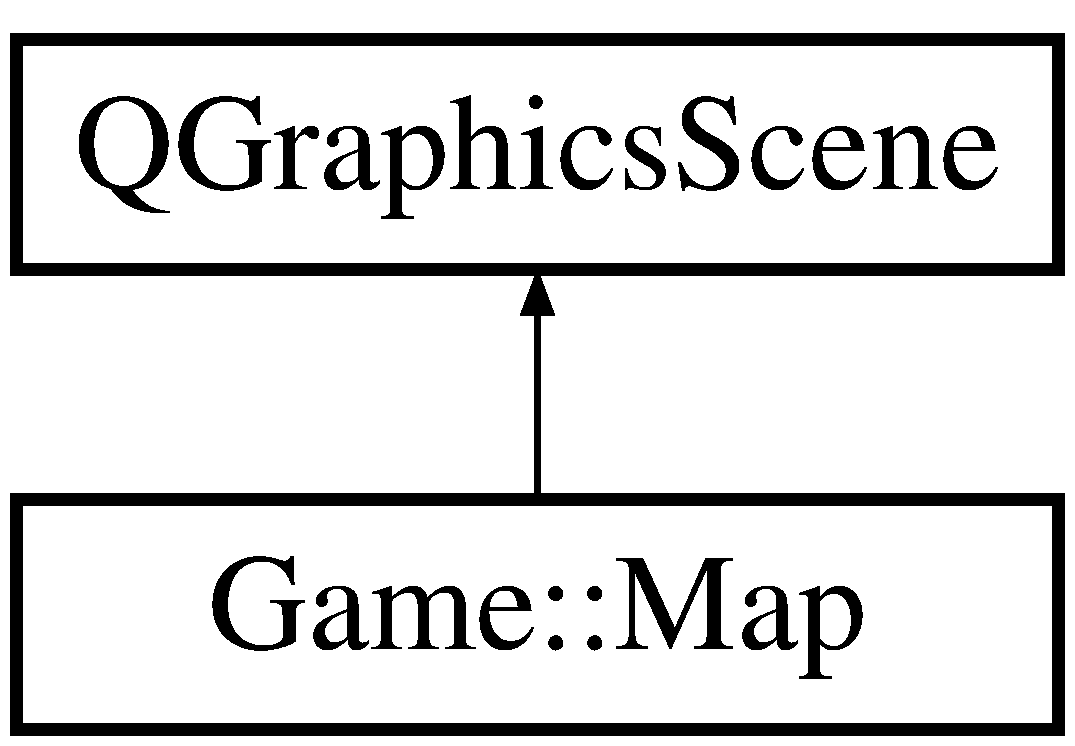
\includegraphics[height=2.000000cm]{class_game_1_1_map}
\end{center}
\end{figure}
\subsection*{Signals}
\begin{DoxyCompactItemize}
\item 
\hypertarget{class_game_1_1_map_a1ae4376a50d7234a5d56cd66ff9686d9}{void \hyperlink{class_game_1_1_map_a1ae4376a50d7234a5d56cd66ff9686d9}{robber\-Found} ()}\label{class_game_1_1_map_a1ae4376a50d7234a5d56cd66ff9686d9}

\begin{DoxyCompactList}\small\item\em robber\-Found emitted when player encounters a robber \end{DoxyCompactList}\item 
\hypertarget{class_game_1_1_map_ac966080c6fe166edf48f150331a6d699}{void \hyperlink{class_game_1_1_map_ac966080c6fe166edf48f150331a6d699}{treasure\-Found} ()}\label{class_game_1_1_map_ac966080c6fe166edf48f150331a6d699}

\begin{DoxyCompactList}\small\item\em treasure\-Found emitted when player encounters a treasure \end{DoxyCompactList}\item 
\hypertarget{class_game_1_1_map_a00eae9638e9b5066954d81b5a8100443}{void \hyperlink{class_game_1_1_map_a00eae9638e9b5066954d81b5a8100443}{nothing\-Found} ()}\label{class_game_1_1_map_a00eae9638e9b5066954d81b5a8100443}

\begin{DoxyCompactList}\small\item\em nothing\-Found emitted when player searches an empty tile \end{DoxyCompactList}\item 
\hypertarget{class_game_1_1_map_a5672c918010de381ccfca5a82a1a1c6a}{void \hyperlink{class_game_1_1_map_a5672c918010de381ccfca5a82a1a1c6a}{built} ()}\label{class_game_1_1_map_a5672c918010de381ccfca5a82a1a1c6a}

\begin{DoxyCompactList}\small\item\em built emitted when player has built a building \end{DoxyCompactList}\item 
void \hyperlink{class_game_1_1_map_ac2461e5dd8dc2ac1e55e727158568a46}{inspect\-Tile} (std\-::string info)
\begin{DoxyCompactList}\small\item\em inspect\-Tile sends the tile's type when emitted \end{DoxyCompactList}\end{DoxyCompactItemize}
\subsection*{Public Member Functions}
\begin{DoxyCompactItemize}
\item 
\hypertarget{class_game_1_1_map_ab35bc9a7f6eb93296195984acc3a7b91}{{\bfseries Map} (Q\-Object $\ast$parent=nullptr, std\-::shared\-\_\-ptr$<$ \hyperlink{class_game_1_1_game_event_handler}{Game\-::\-Game\-Event\-Handler} $>$ event\-Handler=nullptr, std\-::shared\-\_\-ptr$<$ \hyperlink{class_game_1_1_game_object_manager}{Game\-::\-Game\-Object\-Manager} $>$ obj\-Manager=nullptr, std\-::shared\-\_\-ptr$<$ \hyperlink{class_game_1_1_game_map_generator}{Game\-::\-Game\-Map\-Generator} $>$ map\-Generator=nullptr)}\label{class_game_1_1_map_ab35bc9a7f6eb93296195984acc3a7b91}

\item 
void \hyperlink{class_game_1_1_map_ad321530ce793b6aa4e0717f5273e3da5}{mouse\-Move\-Event} (Q\-Graphics\-Scene\-Mouse\-Event $\ast$event) override
\begin{DoxyCompactList}\small\item\em mouse\-Move\-Event highligts the tile that is pointed with cursor \end{DoxyCompactList}\item 
void \hyperlink{class_game_1_1_map_acd0b3b07cca5ead1401cf7eda3ad0e17}{mouse\-Press\-Event} (Q\-Graphics\-Scene\-Mouse\-Event $\ast$mouse\-Event) override
\begin{DoxyCompactList}\small\item\em mouse\-Press\-Event moves player, builds a house, searches and hires workers \end{DoxyCompactList}\item 
\hypertarget{class_game_1_1_map_aca53e9bced941a53bbb8778e051cbad0}{void \hyperlink{class_game_1_1_map_aca53e9bced941a53bbb8778e051cbad0}{draw\-Map} ()}\label{class_game_1_1_map_aca53e9bced941a53bbb8778e051cbad0}

\begin{DoxyCompactList}\small\item\em draw\-Map draw correct tiles spesified by gamemapgenerator \end{DoxyCompactList}\item 
void \hyperlink{class_game_1_1_map_a94213a3927088efe42d57c746feb319b}{move} (std\-::shared\-\_\-ptr$<$ \hyperlink{class_game_1_1_game_tile_base}{Game\-Tile\-Base} $>$ game\-Tile)
\begin{DoxyCompactList}\small\item\em move \end{DoxyCompactList}\item 
void \hyperlink{class_game_1_1_map_a49051ab00e2e5e4d0c8be5f56af39d43}{hire} (std\-::shared\-\_\-ptr$<$ \hyperlink{class_game_1_1_game_tile_base}{Game\-Tile\-Base} $>$ game\-Tile)
\begin{DoxyCompactList}\small\item\em hire \end{DoxyCompactList}\item 
void \hyperlink{class_game_1_1_map_a3e4b9485c9e1298b630e7aa82facb8bc}{build} (std\-::shared\-\_\-ptr$<$ \hyperlink{class_game_1_1_game_tile_base}{Game\-Tile\-Base} $>$ game\-Tile)
\begin{DoxyCompactList}\small\item\em build \end{DoxyCompactList}\item 
void \hyperlink{class_game_1_1_map_ab66fc12a68048a3ddfb8a49316224ded}{search} (std\-::shared\-\_\-ptr$<$ \hyperlink{class_game_1_1_game_tile_base}{Game\-Tile\-Base} $>$ game\-Tile)
\begin{DoxyCompactList}\small\item\em search \end{DoxyCompactList}\item 
void \hyperlink{class_game_1_1_map_ad91ccc0d5e244a66c6f37d0075f6be6d}{inspect} (std\-::shared\-\_\-ptr$<$ \hyperlink{class_game_1_1_game_tile_base}{Game\-Tile\-Base} $>$ game\-Tile)
\begin{DoxyCompactList}\small\item\em inspect \end{DoxyCompactList}\end{DoxyCompactItemize}


\subsection{Detailed Description}
The \hyperlink{class_game_1_1_map}{Map} class draws the map with tiles and player. 

\subsection{Member Function Documentation}
\hypertarget{class_game_1_1_map_a3e4b9485c9e1298b630e7aa82facb8bc}{\index{Game\-::\-Map@{Game\-::\-Map}!build@{build}}
\index{build@{build}!Game::Map@{Game\-::\-Map}}
\subsubsection[{build}]{\setlength{\rightskip}{0pt plus 5cm}void Game\-::\-Map\-::build (
\begin{DoxyParamCaption}
\item[{std\-::shared\-\_\-ptr$<$ {\bf Game\-Tile\-Base} $>$}]{game\-Tile}
\end{DoxyParamCaption}
)}}\label{class_game_1_1_map_a3e4b9485c9e1298b630e7aa82facb8bc}


build 


\begin{DoxyParams}{Parameters}
{\em game\-Tile} & informs the mapgenerator to create a building on the given location \\
\hline
\end{DoxyParams}
\hypertarget{class_game_1_1_map_a49051ab00e2e5e4d0c8be5f56af39d43}{\index{Game\-::\-Map@{Game\-::\-Map}!hire@{hire}}
\index{hire@{hire}!Game::Map@{Game\-::\-Map}}
\subsubsection[{hire}]{\setlength{\rightskip}{0pt plus 5cm}void Game\-::\-Map\-::hire (
\begin{DoxyParamCaption}
\item[{std\-::shared\-\_\-ptr$<$ {\bf Game\-Tile\-Base} $>$}]{game\-Tile}
\end{DoxyParamCaption}
)}}\label{class_game_1_1_map_a49051ab00e2e5e4d0c8be5f56af39d43}


hire 


\begin{DoxyParams}{Parameters}
{\em game\-Tile} & informs the mapgenerator to create a selected worker on the tile \\
\hline
\end{DoxyParams}
\hypertarget{class_game_1_1_map_ad91ccc0d5e244a66c6f37d0075f6be6d}{\index{Game\-::\-Map@{Game\-::\-Map}!inspect@{inspect}}
\index{inspect@{inspect}!Game::Map@{Game\-::\-Map}}
\subsubsection[{inspect}]{\setlength{\rightskip}{0pt plus 5cm}void Game\-::\-Map\-::inspect (
\begin{DoxyParamCaption}
\item[{std\-::shared\-\_\-ptr$<$ {\bf Game\-Tile\-Base} $>$}]{game\-Tile}
\end{DoxyParamCaption}
)}}\label{class_game_1_1_map_ad91ccc0d5e244a66c6f37d0075f6be6d}


inspect 


\begin{DoxyParams}{Parameters}
{\em game\-Tile} & Prints out information of the tile to the game's text box \\
\hline
\end{DoxyParams}
\hypertarget{class_game_1_1_map_ac2461e5dd8dc2ac1e55e727158568a46}{\index{Game\-::\-Map@{Game\-::\-Map}!inspect\-Tile@{inspect\-Tile}}
\index{inspect\-Tile@{inspect\-Tile}!Game::Map@{Game\-::\-Map}}
\subsubsection[{inspect\-Tile}]{\setlength{\rightskip}{0pt plus 5cm}void Game\-::\-Map\-::inspect\-Tile (
\begin{DoxyParamCaption}
\item[{std\-::string}]{info}
\end{DoxyParamCaption}
)\hspace{0.3cm}{\ttfamily [signal]}}}\label{class_game_1_1_map_ac2461e5dd8dc2ac1e55e727158568a46}


inspect\-Tile sends the tile's type when emitted 


\begin{DoxyParams}{Parameters}
{\em info} & \\
\hline
\end{DoxyParams}
\hypertarget{class_game_1_1_map_ad321530ce793b6aa4e0717f5273e3da5}{\index{Game\-::\-Map@{Game\-::\-Map}!mouse\-Move\-Event@{mouse\-Move\-Event}}
\index{mouse\-Move\-Event@{mouse\-Move\-Event}!Game::Map@{Game\-::\-Map}}
\subsubsection[{mouse\-Move\-Event}]{\setlength{\rightskip}{0pt plus 5cm}void Game\-::\-Map\-::mouse\-Move\-Event (
\begin{DoxyParamCaption}
\item[{Q\-Graphics\-Scene\-Mouse\-Event $\ast$}]{event}
\end{DoxyParamCaption}
)\hspace{0.3cm}{\ttfamily [override]}}}\label{class_game_1_1_map_ad321530ce793b6aa4e0717f5273e3da5}


mouse\-Move\-Event highligts the tile that is pointed with cursor 


\begin{DoxyParams}{Parameters}
{\em event} & different colored highlight when building or searching depending on event \\
\hline
\end{DoxyParams}
\hypertarget{class_game_1_1_map_acd0b3b07cca5ead1401cf7eda3ad0e17}{\index{Game\-::\-Map@{Game\-::\-Map}!mouse\-Press\-Event@{mouse\-Press\-Event}}
\index{mouse\-Press\-Event@{mouse\-Press\-Event}!Game::Map@{Game\-::\-Map}}
\subsubsection[{mouse\-Press\-Event}]{\setlength{\rightskip}{0pt plus 5cm}void Game\-::\-Map\-::mouse\-Press\-Event (
\begin{DoxyParamCaption}
\item[{Q\-Graphics\-Scene\-Mouse\-Event $\ast$}]{mouse\-Event}
\end{DoxyParamCaption}
)\hspace{0.3cm}{\ttfamily [override]}}}\label{class_game_1_1_map_acd0b3b07cca5ead1401cf7eda3ad0e17}


mouse\-Press\-Event moves player, builds a house, searches and hires workers 


\begin{DoxyParams}{Parameters}
{\em mouse\-Event} & a click \\
\hline
\end{DoxyParams}
\hypertarget{class_game_1_1_map_a94213a3927088efe42d57c746feb319b}{\index{Game\-::\-Map@{Game\-::\-Map}!move@{move}}
\index{move@{move}!Game::Map@{Game\-::\-Map}}
\subsubsection[{move}]{\setlength{\rightskip}{0pt plus 5cm}void Game\-::\-Map\-::move (
\begin{DoxyParamCaption}
\item[{std\-::shared\-\_\-ptr$<$ {\bf Game\-Tile\-Base} $>$}]{game\-Tile}
\end{DoxyParamCaption}
)}}\label{class_game_1_1_map_a94213a3927088efe42d57c746feb319b}


move 


\begin{DoxyParams}{Parameters}
{\em game\-Tile} & Moves the player to the given location \\
\hline
\end{DoxyParams}
\hypertarget{class_game_1_1_map_ab66fc12a68048a3ddfb8a49316224ded}{\index{Game\-::\-Map@{Game\-::\-Map}!search@{search}}
\index{search@{search}!Game::Map@{Game\-::\-Map}}
\subsubsection[{search}]{\setlength{\rightskip}{0pt plus 5cm}void Game\-::\-Map\-::search (
\begin{DoxyParamCaption}
\item[{std\-::shared\-\_\-ptr$<$ {\bf Game\-Tile\-Base} $>$}]{game\-Tile}
\end{DoxyParamCaption}
)}}\label{class_game_1_1_map_ab66fc12a68048a3ddfb8a49316224ded}


search 


\begin{DoxyParams}{Parameters}
{\em game\-Tile} & Searches a tile and checks if it has a treasure or a robber \\
\hline
\end{DoxyParams}


The documentation for this class was generated from the following files\-:\begin{DoxyCompactItemize}
\item 
map.\-h\item 
map.\-cpp\end{DoxyCompactItemize}

\hypertarget{class_game_1_1_map_window}{\section{Game\-:\-:Map\-Window Class Reference}
\label{class_game_1_1_map_window}\index{Game\-::\-Map\-Window@{Game\-::\-Map\-Window}}
}


The \hyperlink{class_game_1_1_map_window}{Map\-Window} class game window where is map, buttons and messageboxes.  




{\ttfamily \#include $<$mapwindow.\-hh$>$}

Inheritance diagram for Game\-:\-:Map\-Window\-:\begin{figure}[H]
\begin{center}
\leavevmode
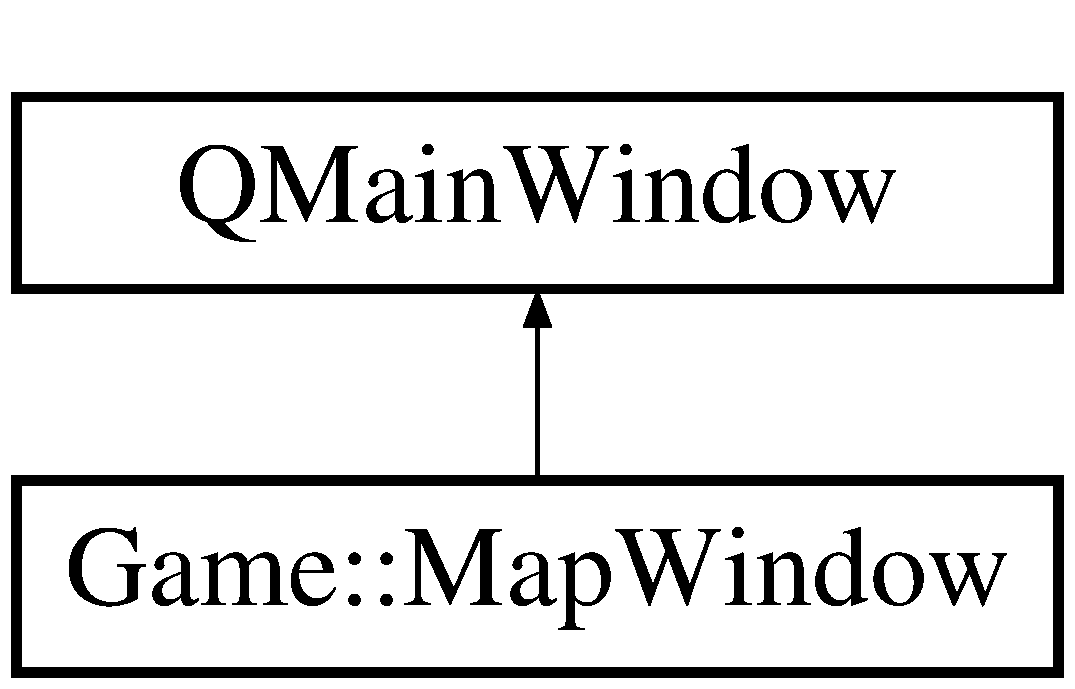
\includegraphics[height=2.000000cm]{class_game_1_1_map_window}
\end{center}
\end{figure}
\subsection*{Public Member Functions}
\begin{DoxyCompactItemize}
\item 
\hypertarget{class_game_1_1_map_window_aada219bb81fc36f618ce6c6db562e21f}{{\bfseries Map\-Window} (Q\-Widget $\ast$parent=nullptr)}\label{class_game_1_1_map_window_aada219bb81fc36f618ce6c6db562e21f}

\item 
void \hyperlink{class_game_1_1_map_window_adba5d7b1e410b80248431586d7e06787}{resize\-Event} (Q\-Resize\-Event $\ast$event) override
\begin{DoxyCompactList}\small\item\em resize\-Event handles events where user changes the mapwindow's size \end{DoxyCompactList}\item 
void \hyperlink{class_game_1_1_map_window_a3ad805cd0011042bae64f7c0680dee75}{show\-Event} (Q\-Show\-Event $\ast$event) override
\begin{DoxyCompactList}\small\item\em show\-Event is called when mapwindow show up on the screen \end{DoxyCompactList}\item 
std\-::string \hyperlink{class_game_1_1_map_window_abddb4e34e8944de58ea55dd263a216e8}{get\-Username} ()
\begin{DoxyCompactList}\small\item\em get\-Username used to get username from starting dialog to the game \end{DoxyCompactList}\item 
void \hyperlink{class_game_1_1_map_window_acf9cb2d5196093123ddbddc77b2e8da8}{key\-Press\-Event} (Q\-Key\-Event $\ast$event) override
\begin{DoxyCompactList}\small\item\em key\-Press\-Event handles events where user presses a key on keyboard \end{DoxyCompactList}\item 
void \hyperlink{class_game_1_1_map_window_a27698728d6b09b81f4921e778700c91b}{mark\-High\-Score} (std\-::string username, int score)
\begin{DoxyCompactList}\small\item\em mark\-High\-Score \end{DoxyCompactList}\end{DoxyCompactItemize}


\subsection{Detailed Description}
The \hyperlink{class_game_1_1_map_window}{Map\-Window} class game window where is map, buttons and messageboxes. 

\subsection{Member Function Documentation}
\hypertarget{class_game_1_1_map_window_abddb4e34e8944de58ea55dd263a216e8}{\index{Game\-::\-Map\-Window@{Game\-::\-Map\-Window}!get\-Username@{get\-Username}}
\index{get\-Username@{get\-Username}!Game::MapWindow@{Game\-::\-Map\-Window}}
\subsubsection[{get\-Username}]{\setlength{\rightskip}{0pt plus 5cm}std\-::string Game\-::\-Map\-Window\-::get\-Username (
\begin{DoxyParamCaption}
{}
\end{DoxyParamCaption}
)}}\label{class_game_1_1_map_window_abddb4e34e8944de58ea55dd263a216e8}


get\-Username used to get username from starting dialog to the game 

\begin{DoxyReturn}{Returns}

\end{DoxyReturn}
\hypertarget{class_game_1_1_map_window_acf9cb2d5196093123ddbddc77b2e8da8}{\index{Game\-::\-Map\-Window@{Game\-::\-Map\-Window}!key\-Press\-Event@{key\-Press\-Event}}
\index{key\-Press\-Event@{key\-Press\-Event}!Game::MapWindow@{Game\-::\-Map\-Window}}
\subsubsection[{key\-Press\-Event}]{\setlength{\rightskip}{0pt plus 5cm}void Game\-::\-Map\-Window\-::key\-Press\-Event (
\begin{DoxyParamCaption}
\item[{Q\-Key\-Event $\ast$}]{event}
\end{DoxyParamCaption}
)\hspace{0.3cm}{\ttfamily [override]}}}\label{class_game_1_1_map_window_acf9cb2d5196093123ddbddc77b2e8da8}


key\-Press\-Event handles events where user presses a key on keyboard 


\begin{DoxyParams}{Parameters}
{\em event} & \\
\hline
\end{DoxyParams}
\hypertarget{class_game_1_1_map_window_a27698728d6b09b81f4921e778700c91b}{\index{Game\-::\-Map\-Window@{Game\-::\-Map\-Window}!mark\-High\-Score@{mark\-High\-Score}}
\index{mark\-High\-Score@{mark\-High\-Score}!Game::MapWindow@{Game\-::\-Map\-Window}}
\subsubsection[{mark\-High\-Score}]{\setlength{\rightskip}{0pt plus 5cm}void Game\-::\-Map\-Window\-::mark\-High\-Score (
\begin{DoxyParamCaption}
\item[{std\-::string}]{username, }
\item[{int}]{score}
\end{DoxyParamCaption}
)}}\label{class_game_1_1_map_window_a27698728d6b09b81f4921e778700c91b}


mark\-High\-Score 


\begin{DoxyParams}{Parameters}
{\em username} & \\
\hline
{\em score} & saves the current score to highscores.\-txt if it's better than the previous one or if there is no score with the given name \\
\hline
\end{DoxyParams}
\hypertarget{class_game_1_1_map_window_adba5d7b1e410b80248431586d7e06787}{\index{Game\-::\-Map\-Window@{Game\-::\-Map\-Window}!resize\-Event@{resize\-Event}}
\index{resize\-Event@{resize\-Event}!Game::MapWindow@{Game\-::\-Map\-Window}}
\subsubsection[{resize\-Event}]{\setlength{\rightskip}{0pt plus 5cm}void Game\-::\-Map\-Window\-::resize\-Event (
\begin{DoxyParamCaption}
\item[{Q\-Resize\-Event $\ast$}]{event}
\end{DoxyParamCaption}
)\hspace{0.3cm}{\ttfamily [override]}}}\label{class_game_1_1_map_window_adba5d7b1e410b80248431586d7e06787}


resize\-Event handles events where user changes the mapwindow's size 


\begin{DoxyParams}{Parameters}
{\em event} & \\
\hline
\end{DoxyParams}
\hypertarget{class_game_1_1_map_window_a3ad805cd0011042bae64f7c0680dee75}{\index{Game\-::\-Map\-Window@{Game\-::\-Map\-Window}!show\-Event@{show\-Event}}
\index{show\-Event@{show\-Event}!Game::MapWindow@{Game\-::\-Map\-Window}}
\subsubsection[{show\-Event}]{\setlength{\rightskip}{0pt plus 5cm}void Game\-::\-Map\-Window\-::show\-Event (
\begin{DoxyParamCaption}
\item[{Q\-Show\-Event $\ast$}]{event}
\end{DoxyParamCaption}
)\hspace{0.3cm}{\ttfamily [override]}}}\label{class_game_1_1_map_window_a3ad805cd0011042bae64f7c0680dee75}


show\-Event is called when mapwindow show up on the screen 


\begin{DoxyParams}{Parameters}
{\em event} & \\
\hline
\end{DoxyParams}


The documentation for this class was generated from the following files\-:\begin{DoxyCompactItemize}
\item 
mapwindow.\-hh\item 
mapwindow.\-cc\end{DoxyCompactItemize}

\hypertarget{class_game_1_1_master_worker}{\section{Game\-:\-:Master\-Worker Class Reference}
\label{class_game_1_1_master_worker}\index{Game\-::\-Master\-Worker@{Game\-::\-Master\-Worker}}
}


The \hyperlink{class_game_1_1_master_worker}{Master\-Worker} class represents master worker.  




{\ttfamily \#include $<$masterworker.\-h$>$}

Inheritance diagram for Game\-:\-:Master\-Worker\-:\begin{figure}[H]
\begin{center}
\leavevmode
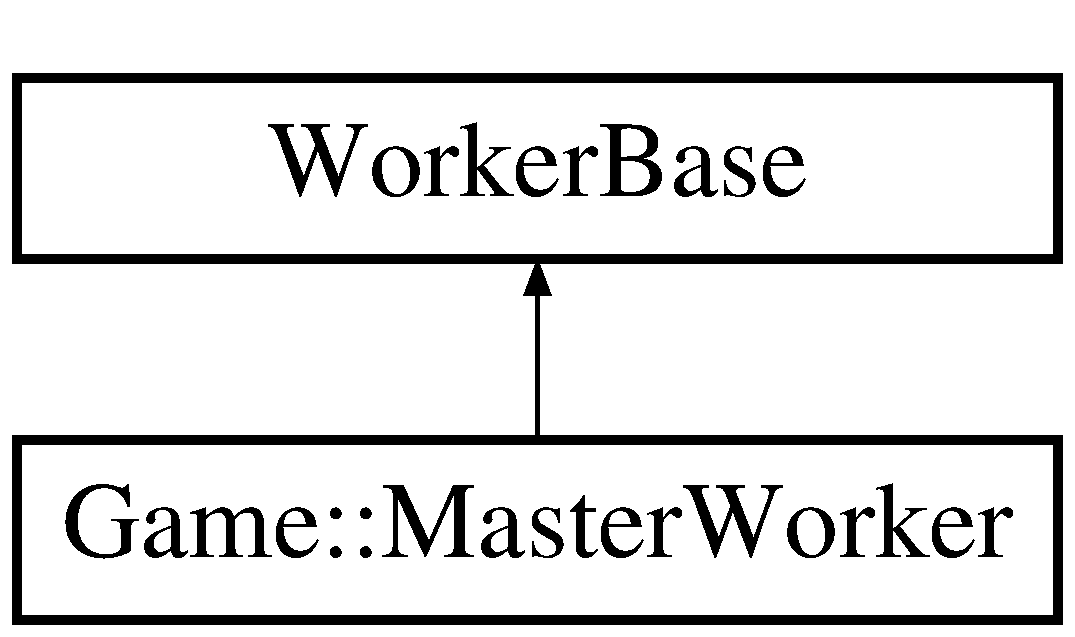
\includegraphics[height=2.000000cm]{class_game_1_1_master_worker}
\end{center}
\end{figure}
\subsection*{Public Member Functions}
\begin{DoxyCompactItemize}
\item 
\hypertarget{class_game_1_1_master_worker_a2968d168a488dedd6f294540287650bd}{{\bfseries Master\-Worker} (const std\-::shared\-\_\-ptr$<$ \hyperlink{class_game_1_1_game_event_handler}{Game\-Event\-Handler} $>$ \&eventhandler, const std\-::shared\-\_\-ptr$<$ \hyperlink{class_game_1_1_game_object_manager}{Game\-Object\-Manager} $>$ \&objectmanager, const std\-::shared\-\_\-ptr$<$ \hyperlink{class_game_1_1_player}{Player} $>$ \&owner, const int \&tilespaces=1, const Course\-::\-Resource\-Map \&cost=Game\-::\-Const\-Game\-Resource\-Map\-::\-M\-W\-\_\-\-R\-E\-C\-R\-U\-I\-T\-M\-E\-N\-T\-\_\-\-C\-O\-S\-T, const Course\-::\-Resource\-Map\-Double \&efficiency=Game\-::\-Const\-Game\-Resource\-Map\-::\-M\-W\-\_\-\-W\-O\-R\-K\-E\-R\-\_\-\-E\-F\-F\-I\-C\-I\-E\-N\-C\-Y)}\label{class_game_1_1_master_worker_a2968d168a488dedd6f294540287650bd}

\item 
\hypertarget{class_game_1_1_master_worker_a2092d711ec017133ca4370b0056feebf}{virtual std\-::string {\bfseries get\-Type} () const override}\label{class_game_1_1_master_worker_a2092d711ec017133ca4370b0056feebf}

\item 
\hypertarget{class_game_1_1_master_worker_aab64502f53bbf8321252eb065bb61398}{virtual void {\bfseries do\-Special\-Action} () override}\label{class_game_1_1_master_worker_aab64502f53bbf8321252eb065bb61398}

\end{DoxyCompactItemize}


\subsection{Detailed Description}
The \hyperlink{class_game_1_1_master_worker}{Master\-Worker} class represents master worker. 

The documentation for this class was generated from the following files\-:\begin{DoxyCompactItemize}
\item 
Workers/masterworker.\-h\item 
Workers/masterworker.\-cpp\end{DoxyCompactItemize}

\hypertarget{class_game_1_1_novice_worker}{\section{Game\-:\-:Novice\-Worker Class Reference}
\label{class_game_1_1_novice_worker}\index{Game\-::\-Novice\-Worker@{Game\-::\-Novice\-Worker}}
}


The \hyperlink{class_game_1_1_novice_worker}{Novice\-Worker} class represents novice worker.  




{\ttfamily \#include $<$noviceworker.\-h$>$}

Inheritance diagram for Game\-:\-:Novice\-Worker\-:\begin{figure}[H]
\begin{center}
\leavevmode
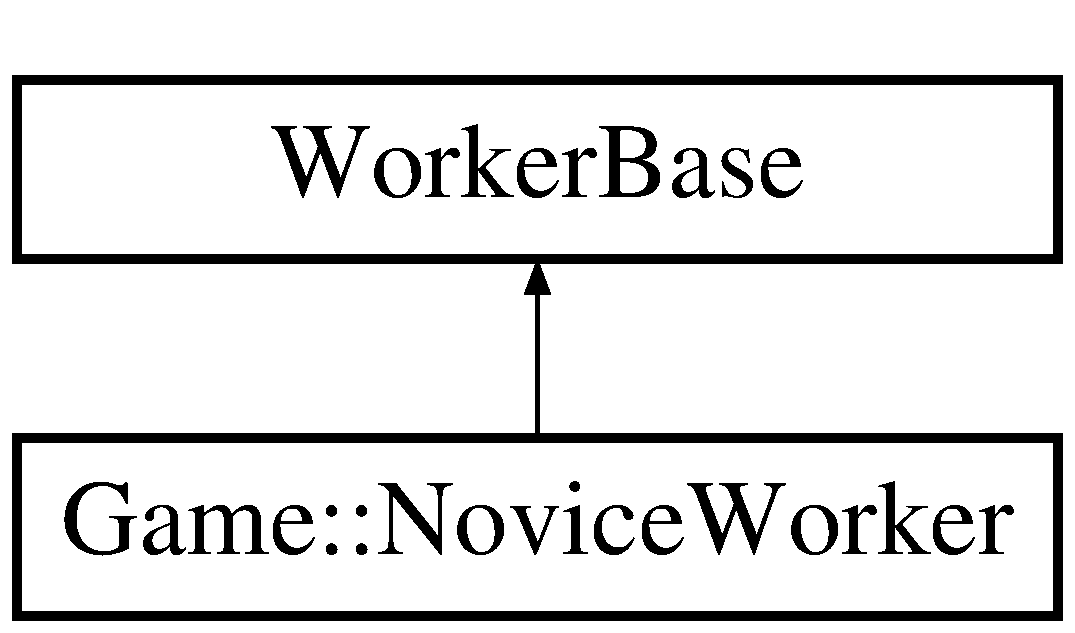
\includegraphics[height=2.000000cm]{class_game_1_1_novice_worker}
\end{center}
\end{figure}
\subsection*{Public Member Functions}
\begin{DoxyCompactItemize}
\item 
\hypertarget{class_game_1_1_novice_worker_ab98dc21c53659739b108abf2f8e0db7a}{{\bfseries Novice\-Worker} (const std\-::shared\-\_\-ptr$<$ \hyperlink{class_game_1_1_game_event_handler}{Game\-Event\-Handler} $>$ \&eventhandler, const std\-::shared\-\_\-ptr$<$ \hyperlink{class_game_1_1_game_object_manager}{Game\-Object\-Manager} $>$ \&objectmanager, const std\-::shared\-\_\-ptr$<$ \hyperlink{class_game_1_1_player}{Player} $>$ \&owner, const int \&tilespaces=1, const Course\-::\-Resource\-Map \&cost=Game\-::\-Const\-Game\-Resource\-Map\-::\-N\-W\-\_\-\-R\-E\-C\-R\-U\-I\-T\-M\-E\-N\-T\-\_\-\-C\-O\-S\-T, const Course\-::\-Resource\-Map\-Double \&efficiency=Game\-::\-Const\-Game\-Resource\-Map\-::\-N\-W\-\_\-\-W\-O\-R\-K\-E\-R\-\_\-\-E\-F\-F\-I\-C\-I\-E\-N\-C\-Y)}\label{class_game_1_1_novice_worker_ab98dc21c53659739b108abf2f8e0db7a}

\item 
\hypertarget{class_game_1_1_novice_worker_a3a008e67e7a009bab02ac9f2a207b7b9}{virtual std\-::string {\bfseries get\-Type} () const override}\label{class_game_1_1_novice_worker_a3a008e67e7a009bab02ac9f2a207b7b9}

\item 
\hypertarget{class_game_1_1_novice_worker_a6cdefbee30452167a84f9a84b451386a}{virtual void {\bfseries do\-Special\-Action} () override}\label{class_game_1_1_novice_worker_a6cdefbee30452167a84f9a84b451386a}

\end{DoxyCompactItemize}


\subsection{Detailed Description}
The \hyperlink{class_game_1_1_novice_worker}{Novice\-Worker} class represents novice worker. 

The documentation for this class was generated from the following files\-:\begin{DoxyCompactItemize}
\item 
Workers/noviceworker.\-h\item 
Workers/noviceworker.\-cpp\end{DoxyCompactItemize}

\hypertarget{class_game_1_1_player}{\section{Game\-:\-:Player Class Reference}
\label{class_game_1_1_player}\index{Game\-::\-Player@{Game\-::\-Player}}
}


The \hyperlink{class_game_1_1_player}{Player} class used for player instance.  




{\ttfamily \#include $<$player.\-h$>$}

Inheritance diagram for Game\-:\-:Player\-:\begin{figure}[H]
\begin{center}
\leavevmode
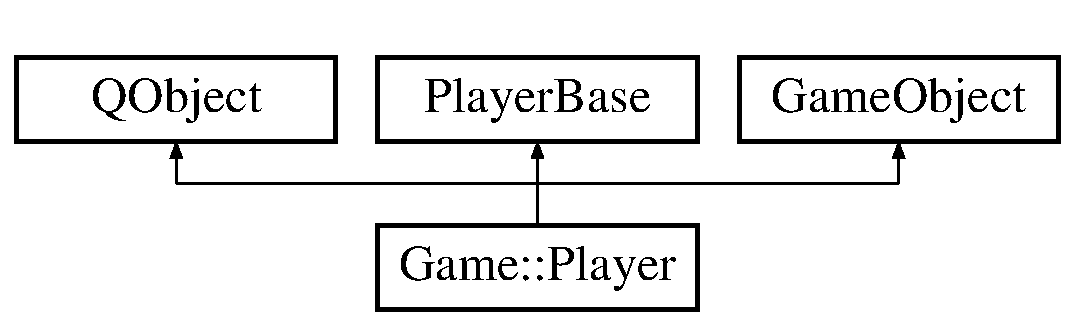
\includegraphics[height=2.000000cm]{class_game_1_1_player}
\end{center}
\end{figure}
\subsection*{Signals}
\begin{DoxyCompactItemize}
\item 
\hypertarget{class_game_1_1_player_ae54c71f3ca4f5001aa790802b046f7bf}{void {\bfseries current\-Money} (int amount)}\label{class_game_1_1_player_ae54c71f3ca4f5001aa790802b046f7bf}

\end{DoxyCompactItemize}
\subsection*{Public Member Functions}
\begin{DoxyCompactItemize}
\item 
\hypertarget{class_game_1_1_player_a1c6a5ecfdb2bc7585a9bb0ad63d5e295}{{\bfseries Player} (const Course\-::\-Coordinate \&coord, const std\-::string \&name=\char`\"{}Adam Smith\char`\"{}, std\-::shared\-\_\-ptr$<$ \hyperlink{class_game_1_1_game_event_handler}{Game\-::\-Game\-Event\-Handler} $>$ handler=nullptr, std\-::shared\-\_\-ptr$<$ \hyperlink{class_game_1_1_game_object_manager}{Game\-::\-Game\-Object\-Manager} $>$ manager=nullptr, const std\-::vector$<$ std\-::shared\-\_\-ptr$<$ Course\-::\-Game\-Object $>$ $>$ objects=\{\}, Q\-Object $\ast$parent=nullptr)}\label{class_game_1_1_player_a1c6a5ecfdb2bc7585a9bb0ad63d5e295}

\item 
\hypertarget{class_game_1_1_player_a0cf49c79fa3670f60ca21137a3085305}{Q\-Pixmap {\bfseries get\-Sprite} ()}\label{class_game_1_1_player_a0cf49c79fa3670f60ca21137a3085305}

\item 
\hypertarget{class_game_1_1_player_a10a40ea56561cbc1532bc448d6459bd7}{Course\-::\-Resource\-Map {\bfseries get\-Resources} ()}\label{class_game_1_1_player_a10a40ea56561cbc1532bc448d6459bd7}

\item 
\hypertarget{class_game_1_1_player_aaba8eb44f579f90c6c07cfe6008e1072}{void {\bfseries modify\-Resources} (Course\-::\-Resource\-Map rmap)}\label{class_game_1_1_player_aaba8eb44f579f90c6c07cfe6008e1072}

\item 
\hypertarget{class_game_1_1_player_ab7f45f2cabc308ab486b9efe296375eb}{void {\bfseries get\-Profit} ()}\label{class_game_1_1_player_ab7f45f2cabc308ab486b9efe296375eb}

\item 
\hypertarget{class_game_1_1_player_ab94597abfe513cb074ee4cb55e96dc0e}{int {\bfseries get\-Starting\-Money} ()}\label{class_game_1_1_player_ab94597abfe513cb074ee4cb55e96dc0e}

\item 
\hypertarget{class_game_1_1_player_a7b5b255cd9f1e8887efdf1f8bdc5e128}{bool {\bfseries has\-Treasure} ()}\label{class_game_1_1_player_a7b5b255cd9f1e8887efdf1f8bdc5e128}

\item 
\hypertarget{class_game_1_1_player_ad6313f98158cdd6d4d5a20b1c21a397a}{void {\bfseries set\-Treasure} (bool t)}\label{class_game_1_1_player_ad6313f98158cdd6d4d5a20b1c21a397a}

\end{DoxyCompactItemize}


\subsection{Detailed Description}
The \hyperlink{class_game_1_1_player}{Player} class used for player instance. 

The documentation for this class was generated from the following files\-:\begin{DoxyCompactItemize}
\item 
player.\-h\item 
player.\-cpp\end{DoxyCompactItemize}

\hypertarget{class_price_window}{\section{Price\-Window Class Reference}
\label{class_price_window}\index{Price\-Window@{Price\-Window}}
}
Inheritance diagram for Price\-Window\-:\begin{figure}[H]
\begin{center}
\leavevmode
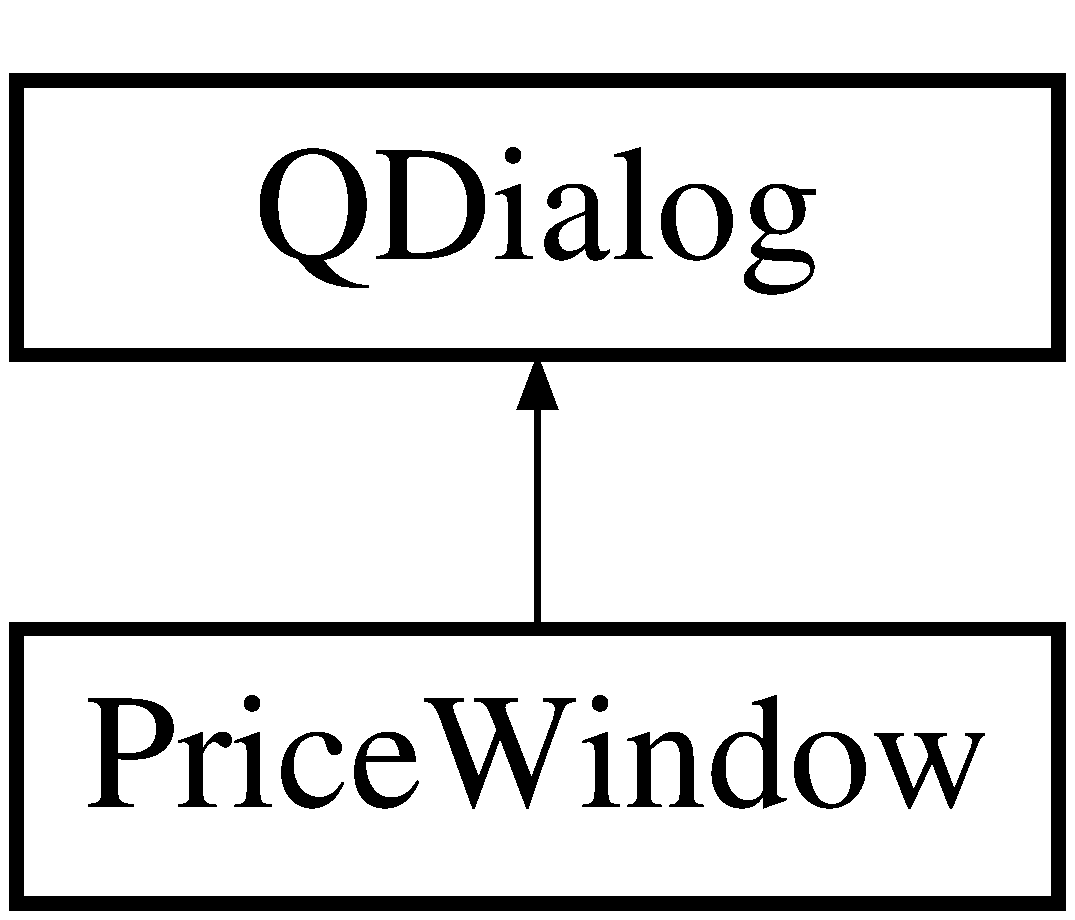
\includegraphics[height=2.000000cm]{class_price_window}
\end{center}
\end{figure}
\subsection*{Public Member Functions}
\begin{DoxyCompactItemize}
\item 
\hypertarget{class_price_window_aa94578d9d5be1c3d71a99aa7d5c98b9f}{{\bfseries Price\-Window} (Q\-Widget $\ast$parent=nullptr)}\label{class_price_window_aa94578d9d5be1c3d71a99aa7d5c98b9f}

\end{DoxyCompactItemize}


The documentation for this class was generated from the following files\-:\begin{DoxyCompactItemize}
\item 
pricewindow.\-h\item 
pricewindow.\-cpp\end{DoxyCompactItemize}

\hypertarget{classrules_window}{\section{rules\-Window Class Reference}
\label{classrules_window}\index{rules\-Window@{rules\-Window}}
}
Inheritance diagram for rules\-Window\-:\begin{figure}[H]
\begin{center}
\leavevmode
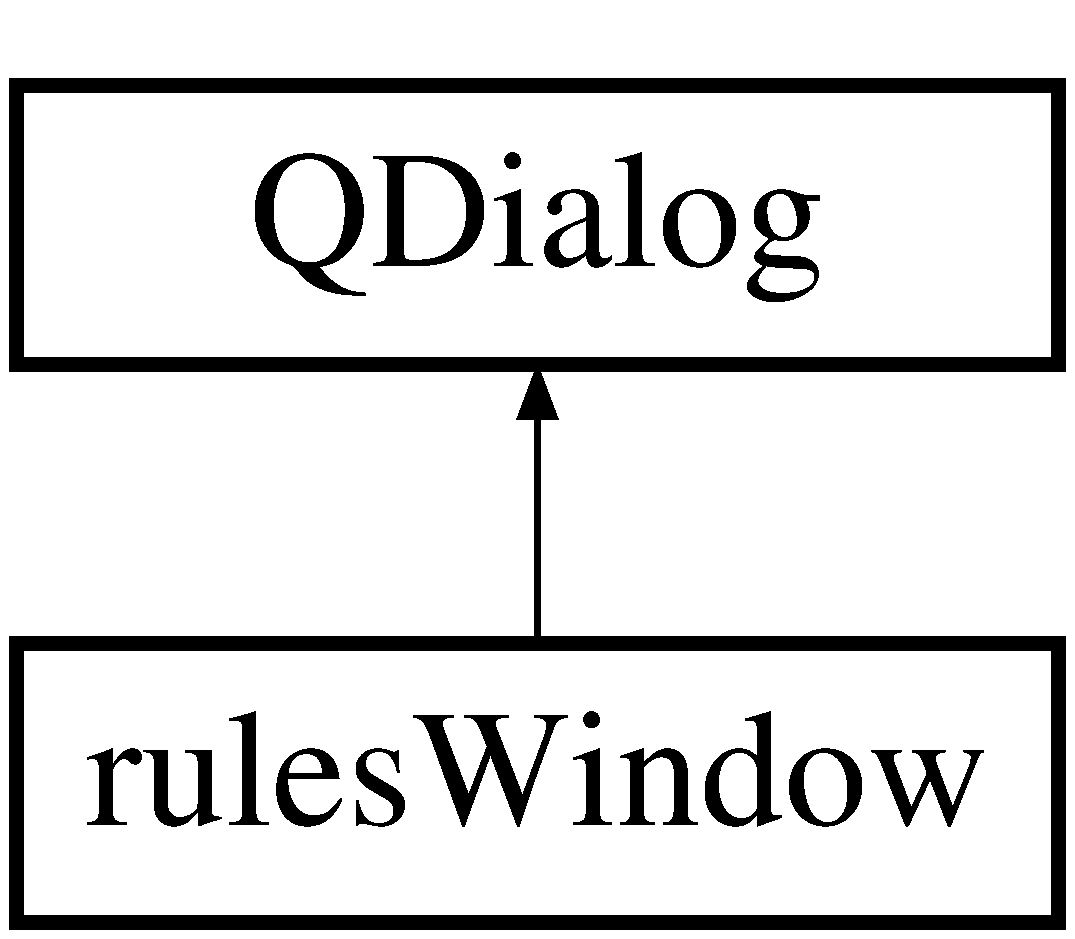
\includegraphics[height=2.000000cm]{classrules_window}
\end{center}
\end{figure}
\subsection*{Public Member Functions}
\begin{DoxyCompactItemize}
\item 
\hypertarget{classrules_window_ab68d6cd4114f873adf625c953d91480b}{{\bfseries rules\-Window} (Q\-Widget $\ast$parent=nullptr)}\label{classrules_window_ab68d6cd4114f873adf625c953d91480b}

\item 
\hypertarget{classrules_window_ab15704667d1b4e8f85f9ab30ddc649ae}{void {\bfseries show\-Rules} ()}\label{classrules_window_ab15704667d1b4e8f85f9ab30ddc649ae}

\item 
\hypertarget{classrules_window_acbe021b744465bfa0edc382f46c12cdb}{void {\bfseries show\-Story} ()}\label{classrules_window_acbe021b744465bfa0edc382f46c12cdb}

\end{DoxyCompactItemize}


The documentation for this class was generated from the following files\-:\begin{DoxyCompactItemize}
\item 
ruleswindow.\-h\item 
ruleswindow.\-cpp\end{DoxyCompactItemize}

\hypertarget{classstart_dialog}{\section{start\-Dialog Class Reference}
\label{classstart_dialog}\index{start\-Dialog@{start\-Dialog}}
}


The \hyperlink{classstart_dialog}{start\-Dialog} class asks for player name and starts the game.  




{\ttfamily \#include $<$startdialog.\-h$>$}

Inheritance diagram for start\-Dialog\-:\begin{figure}[H]
\begin{center}
\leavevmode
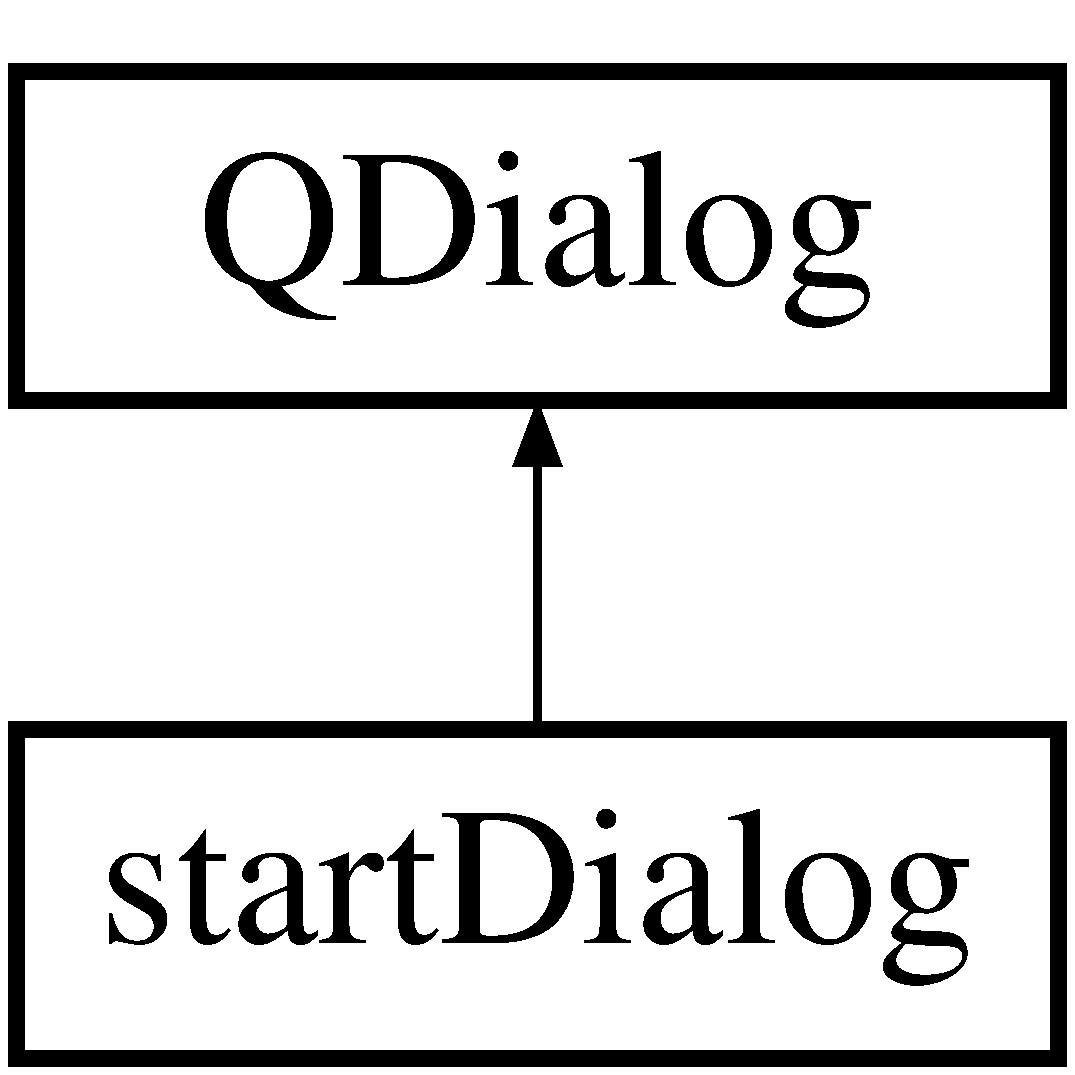
\includegraphics[height=2.000000cm]{classstart_dialog}
\end{center}
\end{figure}
\subsection*{Signals}
\begin{DoxyCompactItemize}
\item 
void \hyperlink{classstart_dialog_a2266e2fa74c0a89fb52cf37838dec5cb}{name\-Confirmed} (std\-::string name)
\begin{DoxyCompactList}\small\item\em name\-Confirmed sends the given username to connected components \end{DoxyCompactList}\end{DoxyCompactItemize}
\subsection*{Public Member Functions}
\begin{DoxyCompactItemize}
\item 
\hypertarget{classstart_dialog_af96dc2ef29556c30a70e575703e09e1c}{{\bfseries start\-Dialog} (Q\-Widget $\ast$parent=nullptr)}\label{classstart_dialog_af96dc2ef29556c30a70e575703e09e1c}

\end{DoxyCompactItemize}
\subsection*{Public Attributes}
\begin{DoxyCompactItemize}
\item 
\hypertarget{classstart_dialog_a0e815d8d32048d4f87483b70a6596021}{Ui\-::start\-Dialog $\ast$ {\bfseries ui}}\label{classstart_dialog_a0e815d8d32048d4f87483b70a6596021}

\end{DoxyCompactItemize}


\subsection{Detailed Description}
The \hyperlink{classstart_dialog}{start\-Dialog} class asks for player name and starts the game. 

\subsection{Member Function Documentation}
\hypertarget{classstart_dialog_a2266e2fa74c0a89fb52cf37838dec5cb}{\index{start\-Dialog@{start\-Dialog}!name\-Confirmed@{name\-Confirmed}}
\index{name\-Confirmed@{name\-Confirmed}!startDialog@{start\-Dialog}}
\subsubsection[{name\-Confirmed}]{\setlength{\rightskip}{0pt plus 5cm}void start\-Dialog\-::name\-Confirmed (
\begin{DoxyParamCaption}
\item[{std\-::string}]{name}
\end{DoxyParamCaption}
)\hspace{0.3cm}{\ttfamily [signal]}}}\label{classstart_dialog_a2266e2fa74c0a89fb52cf37838dec5cb}


name\-Confirmed sends the given username to connected components 


\begin{DoxyParams}{Parameters}
{\em name} & \\
\hline
\end{DoxyParams}


The documentation for this class was generated from the following files\-:\begin{DoxyCompactItemize}
\item 
startdialog.\-h\item 
startdialog.\-cpp\end{DoxyCompactItemize}

\hypertarget{class_game_1_1_town_tile}{\section{Game\-:\-:Town\-Tile Class Reference}
\label{class_game_1_1_town_tile}\index{Game\-::\-Town\-Tile@{Game\-::\-Town\-Tile}}
}
Inheritance diagram for Game\-:\-:Town\-Tile\-:\begin{figure}[H]
\begin{center}
\leavevmode
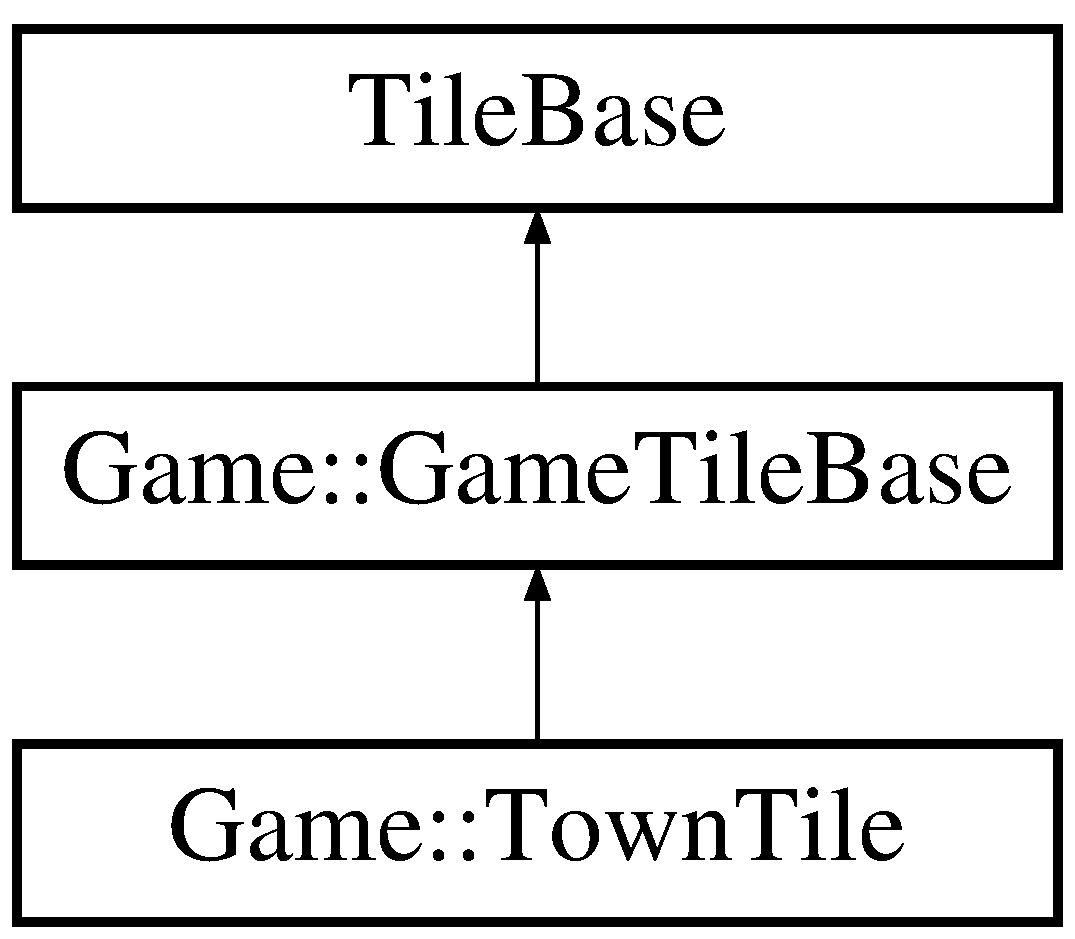
\includegraphics[height=3.000000cm]{class_game_1_1_town_tile}
\end{center}
\end{figure}
\subsection*{Public Member Functions}
\begin{DoxyCompactItemize}
\item 
\hyperlink{class_game_1_1_town_tile_ac0838f0baf66071b049ac8ee9e7f8090}{Town\-Tile} (const Course\-::\-Coordinate \&location, const std\-::shared\-\_\-ptr$<$ \hyperlink{class_game_1_1_game_event_handler}{Game\-Event\-Handler} $>$ \&eventhandler, const std\-::shared\-\_\-ptr$<$ \hyperlink{class_game_1_1_game_object_manager}{Game\-Object\-Manager} $>$ \&objectmanager, const unsigned int \&max\-\_\-build=0, const unsigned int \&max\-\_\-work=0, const Course\-::\-Resource\-Map \&production=Game\-::\-Const\-Game\-Resource\-Map\-::\-E\-M\-P\-T\-Y)
\begin{DoxyCompactList}\small\item\em \hyperlink{class_game_1_1_town_tile}{Town\-Tile}. \end{DoxyCompactList}\item 
virtual std\-::string \hyperlink{class_game_1_1_town_tile_a12b8efcd1bb6f9ef73f54f3493d5866d}{get\-Type} () const override
\begin{DoxyCompactList}\small\item\em get\-Type \end{DoxyCompactList}\end{DoxyCompactItemize}
\subsection*{Additional Inherited Members}


\subsection{Constructor \& Destructor Documentation}
\hypertarget{class_game_1_1_town_tile_ac0838f0baf66071b049ac8ee9e7f8090}{\index{Game\-::\-Town\-Tile@{Game\-::\-Town\-Tile}!Town\-Tile@{Town\-Tile}}
\index{Town\-Tile@{Town\-Tile}!Game::TownTile@{Game\-::\-Town\-Tile}}
\subsubsection[{Town\-Tile}]{\setlength{\rightskip}{0pt plus 5cm}Game\-::\-Town\-Tile\-::\-Town\-Tile (
\begin{DoxyParamCaption}
\item[{const Course\-::\-Coordinate \&}]{location, }
\item[{const std\-::shared\-\_\-ptr$<$ {\bf Game\-Event\-Handler} $>$ \&}]{eventhandler, }
\item[{const std\-::shared\-\_\-ptr$<$ {\bf Game\-Object\-Manager} $>$ \&}]{objectmanager, }
\item[{const unsigned int \&}]{max\-\_\-build = {\ttfamily 0}, }
\item[{const unsigned int \&}]{max\-\_\-work = {\ttfamily 0}, }
\item[{const Course\-::\-Resource\-Map \&}]{production = {\ttfamily Game\-:\-:ConstGameResourceMap\-:\-:EMPTY}}
\end{DoxyParamCaption}
)}}\label{class_game_1_1_town_tile_ac0838f0baf66071b049ac8ee9e7f8090}


\hyperlink{class_game_1_1_town_tile}{Town\-Tile}. 


\begin{DoxyParams}{Parameters}
{\em location} & \\
\hline
{\em eventhandler} & \\
\hline
{\em objectmanager} & \\
\hline
{\em max\-\_\-build} & \\
\hline
{\em max\-\_\-work} & \\
\hline
{\em production} & \\
\hline
\end{DoxyParams}


\subsection{Member Function Documentation}
\hypertarget{class_game_1_1_town_tile_a12b8efcd1bb6f9ef73f54f3493d5866d}{\index{Game\-::\-Town\-Tile@{Game\-::\-Town\-Tile}!get\-Type@{get\-Type}}
\index{get\-Type@{get\-Type}!Game::TownTile@{Game\-::\-Town\-Tile}}
\subsubsection[{get\-Type}]{\setlength{\rightskip}{0pt plus 5cm}std\-::string Game\-::\-Town\-Tile\-::get\-Type (
\begin{DoxyParamCaption}
{}
\end{DoxyParamCaption}
) const\hspace{0.3cm}{\ttfamily [override]}, {\ttfamily [virtual]}}}\label{class_game_1_1_town_tile_a12b8efcd1bb6f9ef73f54f3493d5866d}


get\-Type 

\begin{DoxyReturn}{Returns}
type of the tile as a string 
\end{DoxyReturn}


The documentation for this class was generated from the following files\-:\begin{DoxyCompactItemize}
\item 
Tiles/towntile.\-h\item 
Tiles/towntile.\-cpp\end{DoxyCompactItemize}

\hypertarget{class_game_1_1_water_tile}{\section{Game\-:\-:Water\-Tile Class Reference}
\label{class_game_1_1_water_tile}\index{Game\-::\-Water\-Tile@{Game\-::\-Water\-Tile}}
}


The \hyperlink{class_game_1_1_water_tile}{Water\-Tile} class represents water.  




{\ttfamily \#include $<$watertile.\-h$>$}

Inheritance diagram for Game\-:\-:Water\-Tile\-:\begin{figure}[H]
\begin{center}
\leavevmode
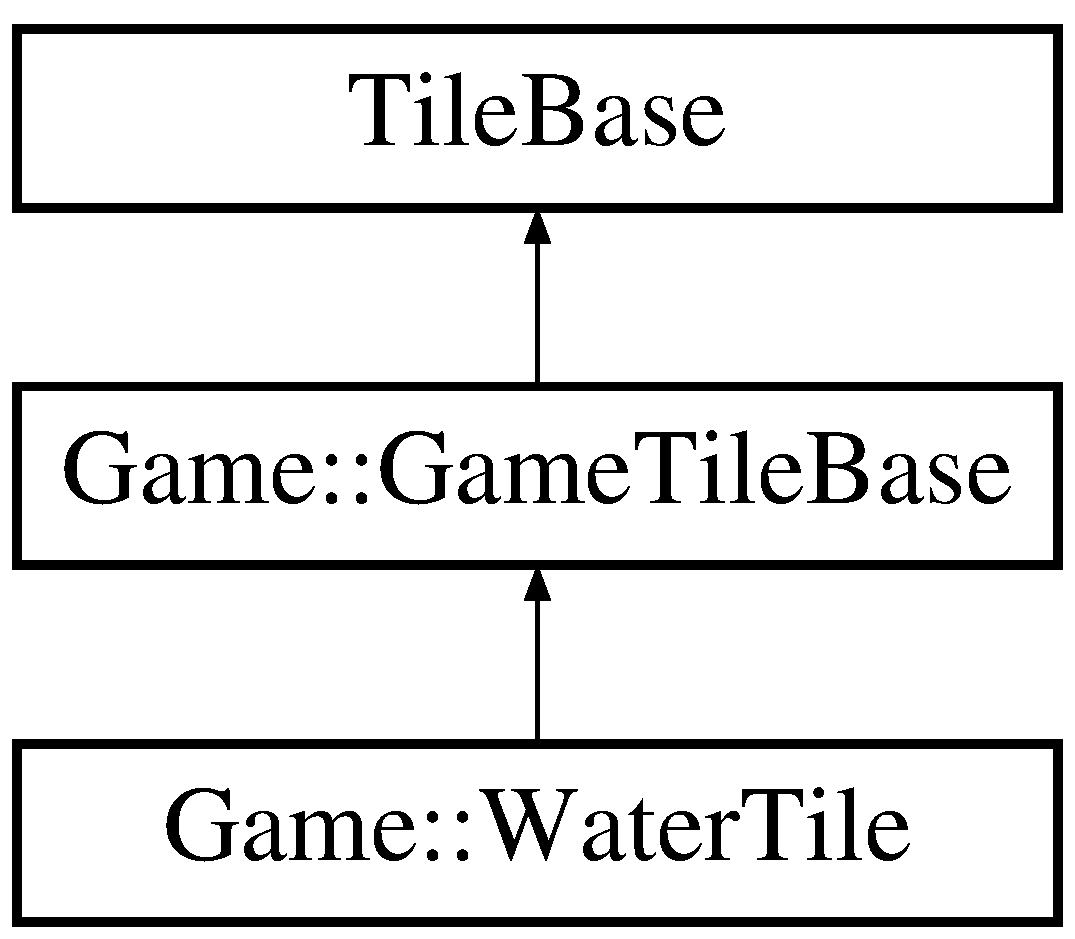
\includegraphics[height=3.000000cm]{class_game_1_1_water_tile}
\end{center}
\end{figure}
\subsection*{Public Member Functions}
\begin{DoxyCompactItemize}
\item 
\hyperlink{class_game_1_1_water_tile_aa32c23d7b999b3a3094f5b5d27f131df}{Water\-Tile} (const Course\-::\-Coordinate \&location, const std\-::shared\-\_\-ptr$<$ \hyperlink{class_game_1_1_game_event_handler}{Game\-Event\-Handler} $>$ \&eventhandler, const std\-::shared\-\_\-ptr$<$ \hyperlink{class_game_1_1_game_object_manager}{Game\-Object\-Manager} $>$ \&objectmanager, const unsigned int \&max\-\_\-build=1, const unsigned int \&max\-\_\-work=5, const Course\-::\-Resource\-Map \&production=Game\-::\-Const\-Game\-Resource\-Map\-::\-T\-I\-L\-E\-\_\-\-B\-P)
\begin{DoxyCompactList}\small\item\em \hyperlink{class_game_1_1_water_tile}{Water\-Tile}. \end{DoxyCompactList}\item 
virtual std\-::string \hyperlink{class_game_1_1_water_tile_ad99fc351f47f0be0120dacecdac11943}{get\-Type} () const override
\begin{DoxyCompactList}\small\item\em get\-Type \end{DoxyCompactList}\end{DoxyCompactItemize}
\subsection*{Additional Inherited Members}


\subsection{Detailed Description}
The \hyperlink{class_game_1_1_water_tile}{Water\-Tile} class represents water. 

\subsection{Constructor \& Destructor Documentation}
\hypertarget{class_game_1_1_water_tile_aa32c23d7b999b3a3094f5b5d27f131df}{\index{Game\-::\-Water\-Tile@{Game\-::\-Water\-Tile}!Water\-Tile@{Water\-Tile}}
\index{Water\-Tile@{Water\-Tile}!Game::WaterTile@{Game\-::\-Water\-Tile}}
\subsubsection[{Water\-Tile}]{\setlength{\rightskip}{0pt plus 5cm}Game\-::\-Water\-Tile\-::\-Water\-Tile (
\begin{DoxyParamCaption}
\item[{const Course\-::\-Coordinate \&}]{location, }
\item[{const std\-::shared\-\_\-ptr$<$ {\bf Game\-Event\-Handler} $>$ \&}]{eventhandler, }
\item[{const std\-::shared\-\_\-ptr$<$ {\bf Game\-Object\-Manager} $>$ \&}]{objectmanager, }
\item[{const unsigned int \&}]{max\-\_\-build = {\ttfamily 1}, }
\item[{const unsigned int \&}]{max\-\_\-work = {\ttfamily 5}, }
\item[{const Course\-::\-Resource\-Map \&}]{production = {\ttfamily Game\-:\-:ConstGameResourceMap\-:\-:TILE\-\_\-BP}}
\end{DoxyParamCaption}
)}}\label{class_game_1_1_water_tile_aa32c23d7b999b3a3094f5b5d27f131df}


\hyperlink{class_game_1_1_water_tile}{Water\-Tile}. 


\begin{DoxyParams}{Parameters}
{\em location} & \\
\hline
{\em eventhandler} & \\
\hline
{\em objectmanager} & \\
\hline
{\em max\-\_\-build} & \\
\hline
{\em max\-\_\-work} & \\
\hline
{\em production} & \\
\hline
\end{DoxyParams}


\subsection{Member Function Documentation}
\hypertarget{class_game_1_1_water_tile_ad99fc351f47f0be0120dacecdac11943}{\index{Game\-::\-Water\-Tile@{Game\-::\-Water\-Tile}!get\-Type@{get\-Type}}
\index{get\-Type@{get\-Type}!Game::WaterTile@{Game\-::\-Water\-Tile}}
\subsubsection[{get\-Type}]{\setlength{\rightskip}{0pt plus 5cm}std\-::string Game\-::\-Water\-Tile\-::get\-Type (
\begin{DoxyParamCaption}
{}
\end{DoxyParamCaption}
) const\hspace{0.3cm}{\ttfamily [override]}, {\ttfamily [virtual]}}}\label{class_game_1_1_water_tile_ad99fc351f47f0be0120dacecdac11943}


get\-Type 

\begin{DoxyReturn}{Returns}
type of the tile as a string 
\end{DoxyReturn}


The documentation for this class was generated from the following files\-:\begin{DoxyCompactItemize}
\item 
Tiles/watertile.\-h\item 
Tiles/watertile.\-cpp\end{DoxyCompactItemize}

%--- End generated contents ---

% Index
\newpage
\phantomsection
\addcontentsline{toc}{part}{Index}
\printindex

\end{document}
